\PassOptionsToPackage{unicode=true}{hyperref} % options for packages loaded elsewhere
\PassOptionsToPackage{hyphens}{url}
%
\documentclass[]{book}
\usepackage{lmodern}
\usepackage{amssymb,amsmath}
\usepackage{ifxetex,ifluatex}
\usepackage{fixltx2e} % provides \textsubscript
\ifnum 0\ifxetex 1\fi\ifluatex 1\fi=0 % if pdftex
  \usepackage[T1]{fontenc}
  \usepackage[utf8]{inputenc}
  \usepackage{textcomp} % provides euro and other symbols
\else % if luatex or xelatex
  \usepackage{unicode-math}
  \defaultfontfeatures{Ligatures=TeX,Scale=MatchLowercase}
\fi
% use upquote if available, for straight quotes in verbatim environments
\IfFileExists{upquote.sty}{\usepackage{upquote}}{}
% use microtype if available
\IfFileExists{microtype.sty}{%
\usepackage[]{microtype}
\UseMicrotypeSet[protrusion]{basicmath} % disable protrusion for tt fonts
}{}
\IfFileExists{parskip.sty}{%
\usepackage{parskip}
}{% else
\setlength{\parindent}{0pt}
\setlength{\parskip}{6pt plus 2pt minus 1pt}
}
\usepackage{hyperref}
\hypersetup{
            pdftitle={Mind, Brain, Body},
            pdfauthor={Emily Towner, Kristen Chu},
            pdfborder={0 0 0},
            breaklinks=true}
\urlstyle{same}  % don't use monospace font for urls
\usepackage{longtable,booktabs}
% Fix footnotes in tables (requires footnote package)
\IfFileExists{footnote.sty}{\usepackage{footnote}\makesavenoteenv{longtable}}{}
\usepackage{graphicx,grffile}
\makeatletter
\def\maxwidth{\ifdim\Gin@nat@width>\linewidth\linewidth\else\Gin@nat@width\fi}
\def\maxheight{\ifdim\Gin@nat@height>\textheight\textheight\else\Gin@nat@height\fi}
\makeatother
% Scale images if necessary, so that they will not overflow the page
% margins by default, and it is still possible to overwrite the defaults
% using explicit options in \includegraphics[width, height, ...]{}
\setkeys{Gin}{width=\maxwidth,height=\maxheight,keepaspectratio}
\setlength{\emergencystretch}{3em}  % prevent overfull lines
\providecommand{\tightlist}{%
  \setlength{\itemsep}{0pt}\setlength{\parskip}{0pt}}
\setcounter{secnumdepth}{5}
% Redefines (sub)paragraphs to behave more like sections
\ifx\paragraph\undefined\else
\let\oldparagraph\paragraph
\renewcommand{\paragraph}[1]{\oldparagraph{#1}\mbox{}}
\fi
\ifx\subparagraph\undefined\else
\let\oldsubparagraph\subparagraph
\renewcommand{\subparagraph}[1]{\oldsubparagraph{#1}\mbox{}}
\fi

% set default figure placement to htbp
\makeatletter
\def\fps@figure{htbp}
\makeatother

\usepackage{booktabs}
\usepackage{amsthm}
\makeatletter
\def\thm@space@setup{%
  \thm@preskip=8pt plus 2pt minus 4pt
  \thm@postskip=\thm@preskip
}
\makeatother
\usepackage[]{natbib}
\bibliographystyle{apalike}

\title{Mind, Brain, Body}
\author{Emily Towner, Kristen Chu}
\date{2020-07-09}

\begin{document}
\maketitle

{
\setcounter{tocdepth}{1}
\tableofcontents
}
\hypertarget{introduction}{%
\chapter{Introduction}\label{introduction}}

The Mind, Brain, Body study looks at how early caregiving experiences influence the emotional, cognitive, and brain development, as well as physical health and wellness.

The study also explores how the bacteria that live inside us (the microbiome) are connected to the development of our brains and bodies.

\hypertarget{wave-1}{%
\chapter{Wave 1}\label{wave-1}}

\hypertarget{checklists}{%
\section{Checklists}\label{checklists}}

\begin{center}\rule{0.5\linewidth}{0.5pt}\end{center}

\hypertarget{initial-checklist}{%
\subsection{Initial Checklist}\label{initial-checklist}}

\textbf{Scheduling and Confirmation}

\begin{itemize}
\tightlist
\item
  Schedule lab session
\item
  Send confirmation email (in templates)

  \begin{itemize}
  \tightlist
  \item
    Attach \href{https://app.box.com/file/630326369239}{Next Steps}
  \end{itemize}
\end{itemize}

\textbf{Enrollment}

\begin{itemize}
\tightlist
\item
  Create participant Box folder using MBB\_template (delete blank README from newly created folder)
\item
  Enroll participant in Wave 1 on REDCap
\item
  Fill participant instrument on REDCap
\item
  Fill counterbalance order on REDCap (Checklist - Lab Session Child Instrument)
\end{itemize}

\textbf{Calendar}

\begin{itemize}
\tightlist
\item
  Create MBB calendar event lab session and invite researchers
\item
  Create DBS calendar event (SAND calendar)
\item
  Create MBB calendar event lab session reminder 1 (email) (1 week prior)
\item
  Create MBB calendar event lab session reminder 2 (email and call) (3 days prior)
\item
  Create MBB calendar event to send home session reminder 1 (email) (1 week after lab session)
\item
  Create MBB calendar event to make home session reminder 1 (call) (8 days after lab session)
\item
  Create MBB calendar event to send home session reminder 2 (email) (10 days after lab session)
\item
  Create MBB calendar event to send home session reminder 3 email (14 days after lab session)
\end{itemize}

\textbf{Reminders}

\begin{itemize}
\tightlist
\item
  Send lab session reminder 1 email (in templates - attach next steps, consent/assent)
\item
  Send lab session reminder 2 email (in templates - attach previous and parking info)
\item
  Confirm participant

  \begin{itemize}
  \tightlist
  \item
    Preferably by phone
  \item
    Update lab session calendar status
  \end{itemize}
\end{itemize}

\begin{center}\rule{0.5\linewidth}{0.5pt}\end{center}

\hypertarget{pre-lab-session-checklist}{%
\subsection{Pre-Lab Session Checklist}\label{pre-lab-session-checklist}}

\hypertarget{lab-session-setup---1-day-prior}{%
\subsubsection{Lab Session Setup - 1 Day Prior}\label{lab-session-setup---1-day-prior}}

\begin{itemize}
\tightlist
\item
  Create participant manila folder
\item
  Print assent/consent forms (Check IRB expiration)

  \begin{itemize}
  \tightlist
  \item
    \href{https://app.box.com/file/630320519707}{Parent consent}
  \item
    Assent - \href{https://app.box.com/file/630320502379}{Child} or \href{https://app.box.com/file/630326888191}{Teen} (None if under 7 years)
  \item
    \href{https://app.box.com/file/630329099729}{Referral consent}
  \item
    \href{https://app.box.com/file/639652767665}{Contact list}
  \item
    \href{https://app.box.com/file/630326424318}{DBS consent}
  \end{itemize}
\item
  Print \href{https://app.box.com/file/630326484181}{MBB Lab-Session Checklist-Child} (Enter counterbalance order)
\item
  Print \href{https://app.box.com/file/630325295018}{MBB Lab-Session Checklist-Parent}
\item
  Print \href{https://app.box.com/file/630326477910}{KSADS Summary Diagnostic Checklists} (Write participant ID on all pages)
\item
  Print and prepare \href{https://app.box.com/file/630326463909}{WASI Form} (Enter starting point; write participant ID on all pages)
\item
  Print and prepare \href{https://app.box.com/file/630318060264}{WIAT Form} \& \href{https://app.box.com/file/630326404817}{Booklet} (Enter starting point; Write participant ID on all pages)
\item
  Print \href{https://app.box.com/file/630322810250}{Memory Intrusion Scratch Paper}
\item
  Print and insert \href{https://app.box.com/file/630326499609}{Bristol Stool Scale} (MBB Specific Version)
\item
  Print and fill in codes on \href{https://app.box.com/file/630317204624}{Participant Info Brochure}
\item
  File participant manila folder in front section of file cabinet (Upcoming)
\item
  Charge

  \begin{itemize}
  \tightlist
  \item
    iPads
  \item
    iPad pencils
  \item
    Biopac transmitters
  \item
    VR headset (Check remote battery)
  \item
    Audio recorders
  \end{itemize}
\item
  Make sure audio recorder batteries have enough charge
\item
  Label electrodes with color stickers

  \begin{itemize}
  \tightlist
  \item
    Blue=EGG
  \item
    Yellow=ECG
  \end{itemize}
\item
  Make \href{https://app.box.com/file/630320259767}{participant name tags}
\item
  Print \href{https://app.box.com/file/630326568873}{Payment Receipt Template}
\item
  Assemble home kit

  \begin{itemize}
  \tightlist
  \item
    Insert gut kit
  \item
    Insert toilet hat
  \item
    Insert oral kit
  \item
    Insert biohazard bag
  \item
    Insert Bristol Stool Scale
  \item
    Label all items with participant ID (in sharpie)
  \item
    Insert MBB info cards
  \item
    Attach FedEx slip to mailer
  \item
    Label mailer with ``Exempt human specimen'' (in sharpie)
  \end{itemize}
\end{itemize}

\begin{center}\rule{0.5\linewidth}{0.5pt}\end{center}

\hypertarget{lab-session-setup---1-hour-prior}{%
\subsubsection{Lab Session Setup - 1 Hour Prior}\label{lab-session-setup---1-hour-prior}}

\begin{itemize}
\tightlist
\item
  Place in Rainbow Room

  \begin{itemize}
  \tightlist
  \item
    Consent/assent/DBS/contact on clipboard with pens
  \item
    Consent protocol
  \item
    \href{https://app.box.com/file/630327764749}{Pleasant Events Checklist and Issues Checklist}
  \end{itemize}
\item
  Place WASI \& books (2)/WIAT \& card/protocol in testing room
\item
  Place audio recorders in testing rooms
\item
  Attach researcher documents to clipboards

  \begin{itemize}
  \tightlist
  \item
    Child - Checklist, Memory Intrusion notes
  \item
    Parent - Checklist, KSADS summary
  \end{itemize}
\item
  Turn iPads on airplane mode and WiFi off
\item
  Clear and setup KSADS on iPad (duplicate blanks)
\item
  Photograph FedEx slip
\item
  Pre-load questionnaires on computers

  \begin{itemize}
  \tightlist
  \item
    (Parent and Child; under 8-laminated faces)
  \end{itemize}
\item
  Pre-load physiology data templates (8)
\item
  Move physiology station near Rainbow Room
\item
  Move iPad and iPad stand near Rainbow Room
\item
  Insert Participant Info Brochure in home kit
\item
  Assemble hair sample materials
\item
  Prep blood spot kit
\end{itemize}

\begin{center}\rule{0.5\linewidth}{0.5pt}\end{center}

\hypertarget{lab-session-checklist}{%
\subsection{Lab Session Checklist}\label{lab-session-checklist}}

\hypertarget{child}{%
\subsubsection{Child}\label{child}}

\begin{itemize}
\tightlist
\item
  Assent
\item
  Physiology setup
\item
  Parent-child observation (video record)
\item
  Drink bottle of water
\item
  Memory intrusion (audio record)
\item
  Halloween training
\item
  Characters (monsters/aliens)
\item
  Halloween test
\item
  Discrimination (run 1 of 3) *no physio
\item
  Conditioning (sound)
\item
  Discrimination (run 2 of 3) *no physio
\item
  Height
\item
  Hair sample
\item
  Weight
\item
  Saliva sample
\item
  Memory generalization training (audio record)
\item
  Extinction
\item
  Discrimination (run 3 of 3) *no physio
\item
  Memory generalization test
\item
  Waist circumference
\item
  Snack and water break
\item
  WASI (audio record)
\item
  WIAT (audio record)
\item
  Blood sample
\item
  Questionnaires
\item
  Prize
\end{itemize}

\hypertarget{parent}{%
\subsubsection{Parent}\label{parent}}

\begin{itemize}
\tightlist
\item
  Consent
\item
  Parent-child observation (video record)
\item
  KSADS (audio record)
\item
  Transfer observation video/KSADS audio recording
\item
  Questionnaires

  \begin{itemize}
  \tightlist
  \item
    Parent Proxy or Parent Self
  \end{itemize}
\item
  Home kit issues and explained

  \begin{itemize}
  \tightlist
  \item
    Take photo of Fedex label
  \end{itemize}
\item
  Payment issued and signed

  \begin{itemize}
  \tightlist
  \item
    Take photo of receipt
  \end{itemize}
\end{itemize}

\begin{center}\rule{0.5\linewidth}{0.5pt}\end{center}

\hypertarget{post-lab-session-checklist}{%
\subsection{Post-Lab Session Checklist}\label{post-lab-session-checklist}}

\hypertarget{clean-up}{%
\subsubsection{Clean Up}\label{clean-up}}

\begin{itemize}
\tightlist
\item
  Tidy lab
\item
  Disinfectant spray
\item
  Disinfectant wipe
\end{itemize}

\hypertarget{notes}{%
\subsubsection{Notes}\label{notes}}

\begin{itemize}
\tightlist
\item
  Make note in Trello of issues to discuss (if needed) (titled: MBB\#\#\# Lab Session Discussion)
\end{itemize}

\hypertarget{sample-storage}{%
\subsubsection{Sample Storage}\label{sample-storage}}

\begin{itemize}
\tightlist
\item
  Label and leave blood sample to dry
\item
  Store blood sample
\item
  Label and store hair sample
\item
  Label and store saliva sample
\item
  Create and assign Trello reminder to store blood sample
\item
  Update sample storage log on Box (after lab session)
\end{itemize}

\hypertarget{filing}{%
\subsubsection{Filing}\label{filing}}

\begin{itemize}
\tightlist
\item
  File consent and assent forms in filing cabinet (consent manila folder)
\item
  File contact list in filing cabinet (contact list manila folder)
\item
  Log participant payment in reimbursement log book
\item
  File payment receipt photo in Box payment folder
\item
  File FedEx tracking photo in Box folder
\end{itemize}

\hypertarget{data-entry}{%
\subsubsection{Data Entry}\label{data-entry}}

\begin{itemize}
\tightlist
\item
  Transfer and rename video recordings to external hard drive (delete originals)
\item
  Transfer and rename audio recordings to external hard drive (delete originals)
\item
  Copy behavioral task data to participant folder (raw)
\item
  Copy physiology task data to participant folder
\item
  Save and upload KSADS screen from iPad to participant Box folder
\item
  Save and upload any KSADS supplements from iPad to participant Box folder
\end{itemize}

\begin{center}\rule{0.5\linewidth}{0.5pt}\end{center}

\hypertarget{final-checklist}{%
\subsection{Final Checklist}\label{final-checklist}}

\hypertarget{scoring}{%
\subsubsection{Scoring}\label{scoring}}

\begin{itemize}
\tightlist
\item
  Fill out KSADS Summary Diagnostic Checklists
\item
  Score WASI
\item
  Score WIAT
\end{itemize}

\hypertarget{filing-1}{%
\subsubsection{Filing}\label{filing-1}}

\begin{itemize}
\tightlist
\item
  Scan DBS consent and file in participant Box folder
\item
  Scan Memory Intrusion Notes and file in participant Box folder
\item
  Scan KSADS Summary Diagnostic Checklist and file in participant Box folder
\item
  Scan lab session checklists (parent \& child) and file in participant Box folder
\item
  Scan WASI/WIAT (once scored) and file in participant Box folder
\item
  Make low-res parent-child interaction video and save on BABLab Drive
\item
  Burn all audio and video (low res) files to CD and label/store CD in binder
\item
  Check video transfer and delete original
\item
  Check audio transfers and delete originals
\end{itemize}

\hypertarget{data-entry-1}{%
\subsubsection{Data Entry}\label{data-entry-1}}

\begin{itemize}
\tightlist
\item
  Enter contact list information into recruitment database
\item
  Enter KSADS Summary Diagnostic Checklist data to REDCap
\item
  Enter height, weight, waist to REDCap
\item
  Score and enter WASI data to REDCap
\item
  Score and enter WIAT data to REDCap
\item
  Enter Memory Intrusion Notes to REDCap
\item
  Enter lab session checklist - Child data to REDCap
\item
  Enter lab session checklist - Parent data to REDCap
\end{itemize}

\hypertarget{reminders}{%
\subsubsection{Reminders}\label{reminders}}

\begin{itemize}
\tightlist
\item
  Home session reminder 1 email sent
\item
  Reminder 1 phone call made
\item
  Home session reminder 2 email sent
\item
  Home session reminder 3 email sent
\end{itemize}

\hypertarget{home-session}{%
\subsubsection{Home Session}\label{home-session}}

\begin{itemize}
\tightlist
\item
  Halloween test delay
\item
  Memory Generalization test delay
\item
  Stool kit received
\item
  Bristol Stool Scale data received
\item
  ASA
\end{itemize}

\hypertarget{data-entry-2}{%
\subsubsection{Data Entry}\label{data-entry-2}}

\begin{itemize}
\tightlist
\item
  Enter home session checklist child data to REDCap
\item
  Download and upload ASA data to participant Box folder
\item
  Scan and upload Bristol Stool Scale to Box
\item
  Enter Bristol Stool Scale data to REDCap
\end{itemize}

\hypertarget{sample-storage-1}{%
\subsubsection{Sample Storage}\label{sample-storage-1}}

\begin{itemize}
\tightlist
\item
  Label and store stool sample (add data quality to REDCap)
\item
  Update sample storage log on Box (once all received)
\item
  Upload sample photo to Box
\end{itemize}

\hypertarget{reimbursement}{%
\subsubsection{Reimbursement}\label{reimbursement}}

\begin{itemize}
\tightlist
\item
  Send thank you email (in templates)

  \begin{itemize}
  \tightlist
  \item
    Attach letter, certificate, and parent report
  \end{itemize}
\item
  Mail gift card

  \begin{itemize}
  \tightlist
  \item
    Include thank you letter, certificates, and any additional stool kits if needed
  \end{itemize}
\end{itemize}

\hypertarget{data-quality}{%
\subsubsection{Data Quality}\label{data-quality}}

\begin{itemize}
\tightlist
\item
  Data quality check 1
\item
  Data quality check 2
\item
  Data audit
\end{itemize}

\hypertarget{retention}{%
\subsubsection{Retention}\label{retention}}

\begin{itemize}
\tightlist
\item
  Prep report card
\item
  Send report card email (in templates - attach report card)
\item
  Update participant Wave 2 status
\end{itemize}

\begin{enumerate}
\def\labelenumi{\arabic{enumi}.}
\tightlist
\item
  Open a participant data folder
\end{enumerate}

\begin{figure}
\centering
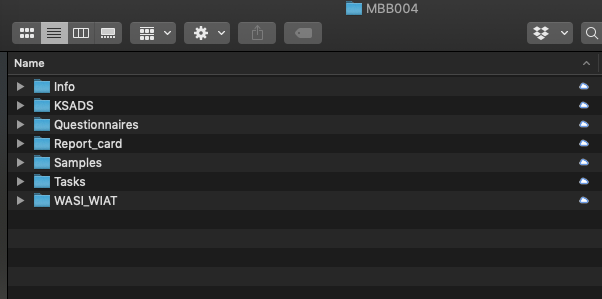
\includegraphics{images/final_checklist/report_cards/1.png}
\caption{}
\end{figure}

\begin{enumerate}
\def\labelenumi{\arabic{enumi}.}
\setcounter{enumi}{1}
\tightlist
\item
  Navigate to the report card folder and rename the template file - MBB999 to the relevant participant - and open the file
\end{enumerate}

\begin{figure}
\centering
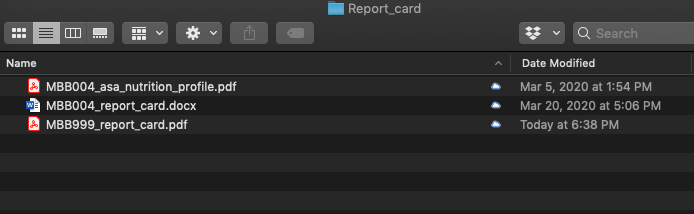
\includegraphics{images/final_checklist/report_cards/2.png}
\caption{}
\end{figure}

\begin{enumerate}
\def\labelenumi{\arabic{enumi}.}
\setcounter{enumi}{2}
\tightlist
\item
  If an ASA nutrition report has been generated for this participant, delete page 4 of the pdf. If no ASA nutrition report has been generated, delete page 3 of the pdf.
\end{enumerate}

\begin{figure}
\centering
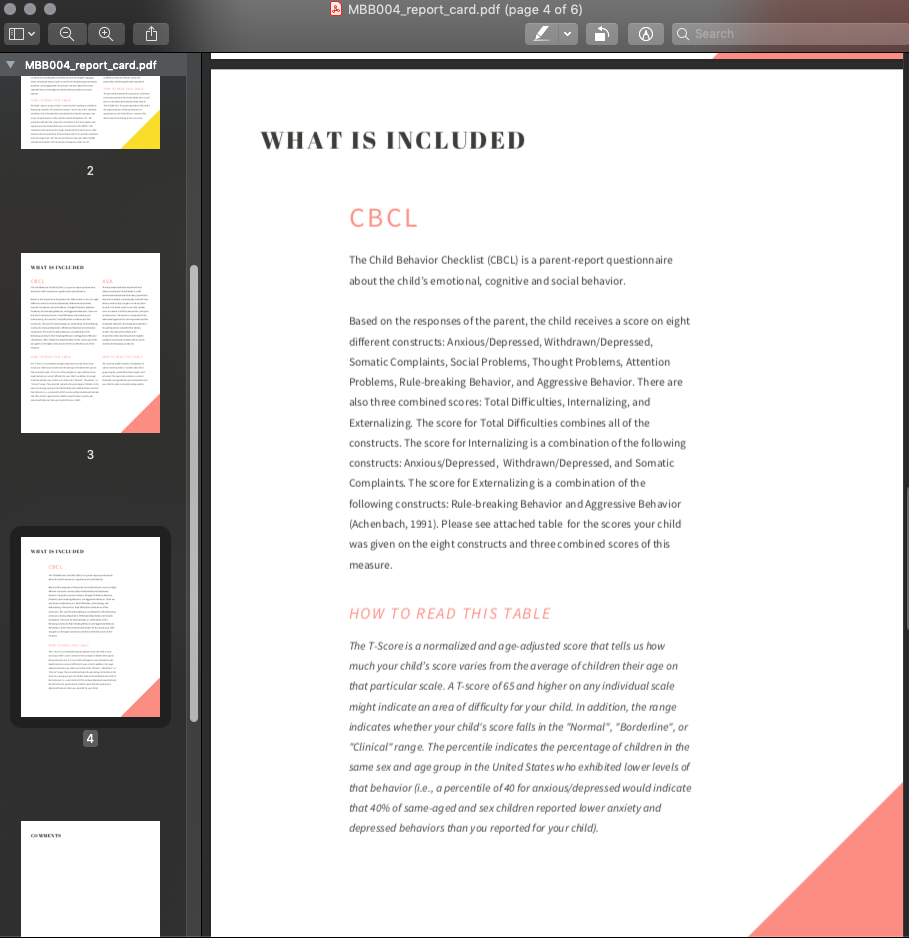
\includegraphics{images/final_checklist/report_cards/3.png}
\caption{}
\end{figure}

\begin{enumerate}
\def\labelenumi{\arabic{enumi}.}
\setcounter{enumi}{3}
\tightlist
\item
  Navigate to the last pge of the pdf, and fill in the scores for this participant. You can type directly on the page - it is a fillable form.
\end{enumerate}

\begin{figure}
\centering
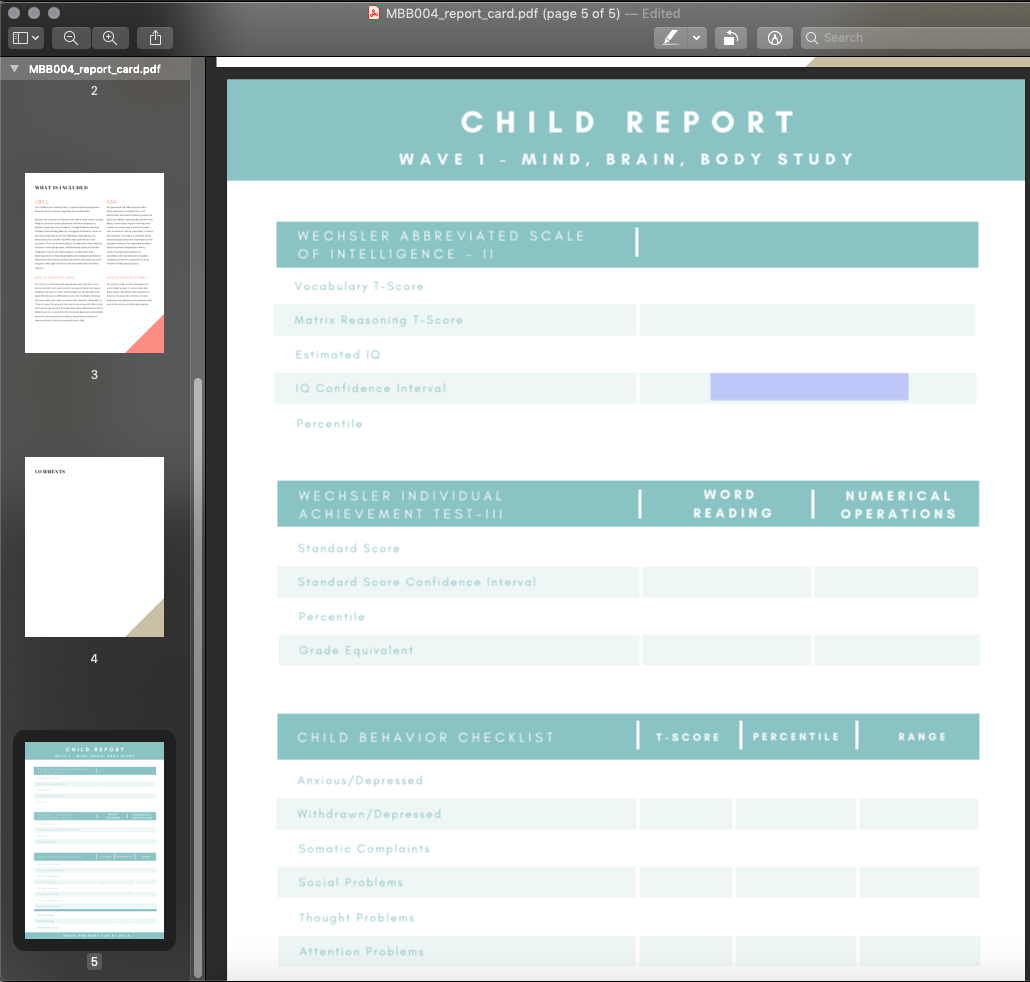
\includegraphics{images/final_checklist/report_cards/4.png}
\caption{}
\end{figure}

\begin{enumerate}
\def\labelenumi{\arabic{enumi}.}
\setcounter{enumi}{4}
\tightlist
\item
  After you have entered the data, it should look like this
\end{enumerate}

\begin{figure}
\centering
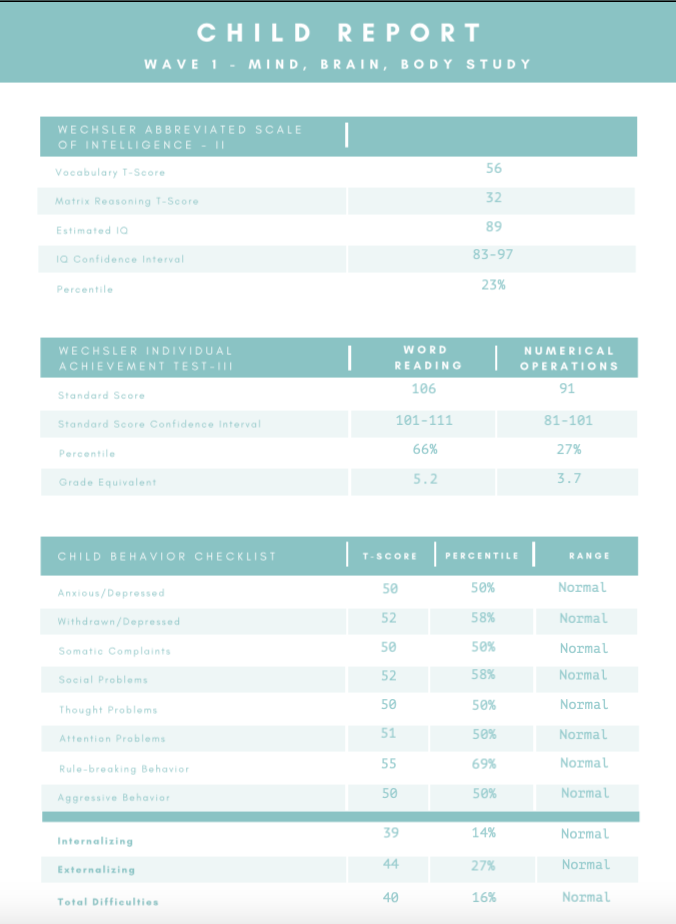
\includegraphics{images/final_checklist/report_cards/5.png}
\caption{}
\end{figure}

\begin{enumerate}
\def\labelenumi{\arabic{enumi}.}
\setcounter{enumi}{5}
\tightlist
\item
  If there are any comments, enter them on the comments page.
\end{enumerate}

\begin{itemize}
\item
  For example, if any NA's are present due to less than 70\% of data for that subset being available to calculate a score - note that here. Or, for example if the child was too young to receive a grade based score, you could note the aged based reading of the table here.
\item
  If there are no comments, delete this page.
\end{itemize}

\begin{figure}
\centering

\includegraphics{images/final_checklist/report_cards/6.png}
\caption{}
\end{figure}

\begin{enumerate}
\def\labelenumi{\arabic{enumi}.}
\setcounter{enumi}{6}
\tightlist
\item
  \textbf{Important} - Once you have completed the edits to the pdf, you must follow these steps to ``lock'' the data so that it is no longer editable before sending to the participant. To do so, click file/print/PDF/Save as PDF. Save the PDF to your desktop, then replace the original PDF with the desktop version.
\end{enumerate}

\begin{figure}
\centering
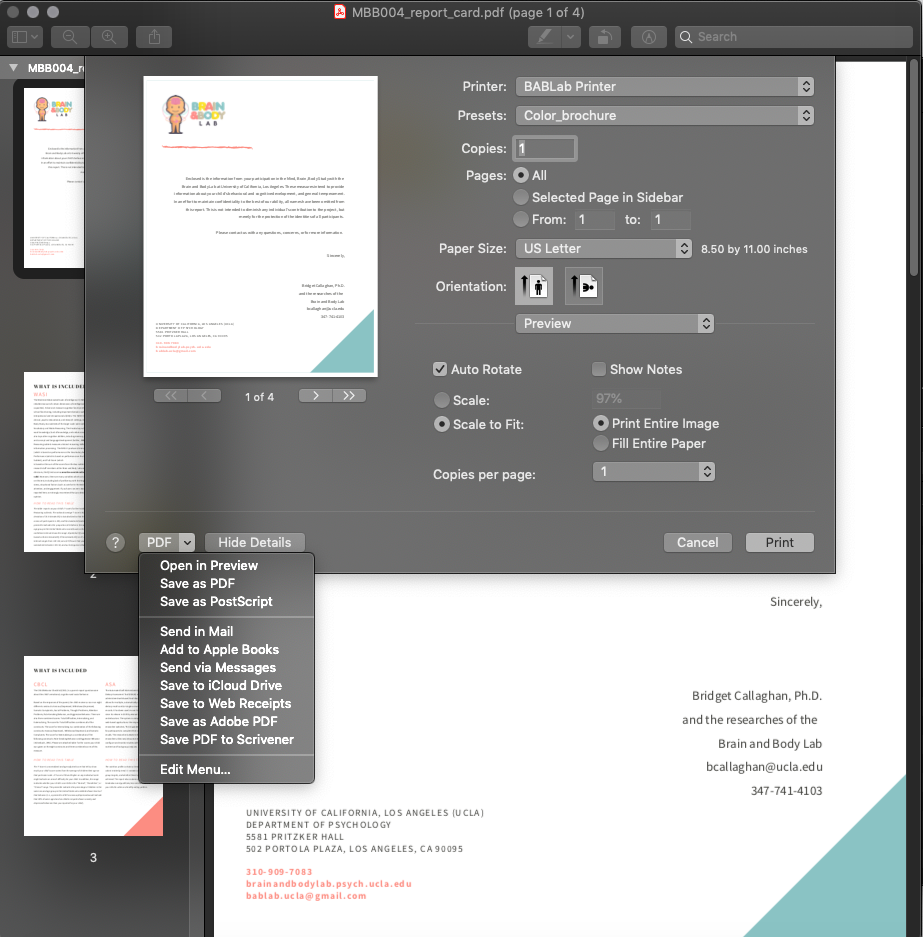
\includegraphics{images/final_checklist/report_cards/7.png}
\caption{}
\end{figure}

\begin{enumerate}
\def\labelenumi{\arabic{enumi}.}
\setcounter{enumi}{7}
\tightlist
\item
  The report card is now ready to be sent to the participant.
\end{enumerate}

\begin{center}\rule{0.5\linewidth}{0.5pt}\end{center}

\hypertarget{childteen-parent-general-protocols}{%
\section{Child/Teen \& Parent General Protocols}\label{childteen-parent-general-protocols}}

\hypertarget{consent-assent}{%
\subsection{Consent \& Assent}\label{consent-assent}}

Once the parent and child/teen come into the lab, seat them in the Rainbow Room on the couch for consenting (parent) and assenting (child aged 7+ or teen).

Make some small talk - Ask the participant how they got here. If they have participated before in research. Offer them a bottle of water. Thank them for coming and for giving up their weekend to help science.

Tell the parent and child that the first thing you are going to do is go over all of the things they will do today, and have them sign the consent and assent forms.

Speak to them and direct them through the whole process.

\hypertarget{things-you-will-do-in-the-lab}{%
\subsubsection{Things you will do in the lab}\label{things-you-will-do-in-the-lab}}

\begin{itemize}
\tightlist
\item
  Stick stickers on you to measure heart rate, sweat, stomach muscles.
\item
  Sit with parent and talk about fun things and hard things (filming).
\item
  Parent stays in room and answers more questions.
\item
  Child goes next door to play computer games (look at pictures, watch movies). Some of the movies and pictures will be a little bit scary, others sad, others boring.
\item
  One of the games involves a loud annoying noise, we will adjust it for you.
\item
  You will also do some other games on paper and pencil - like puzzle and word games
\item
  You will answer some questionnaires
\item
  We will also measure your height, weight, and waist circumference.
\item
  We will take three biological samples:

  \begin{itemize}
  \tightlist
  \item
    Hair - stress hormones
  \item
    Saliva - microbiome
  \item
    Blood - immune - wear goggles
  \end{itemize}
\item
  Do you get sick or dizzy when you see blood or hurt yourself?
\item
  If we need to, can we prick two fingers?
\item
  When you are done with all of that, you will get a big prize, then we will pay you and you will go home.
\item
  You will get \$45 for the work you put in today.
\end{itemize}

\hypertarget{things-you-will-do-at-home}{%
\subsubsection{Things you will do at home}\label{things-you-will-do-at-home}}

Child

\begin{itemize}
\tightlist
\item
  Poop sample - microbiome
\item
  Stool scale
\item
  Memory game - to see what you remember from lab.
\end{itemize}

Parent

\begin{itemize}
\tightlist
\item
  24 hour food recall
\end{itemize}

When you complete the poop sample and the games at home, we will pay you another \$20 in the form of a giftcard.

\hypertarget{things-to-know}{%
\subsubsection{Things to know}\label{things-to-know}}

You are a volunteer, which means that you do not have to do anything, or say anything that makes you uncomfortable. We would like you to try everything you can, and to do your best, but if there are things you absolutely do not want to do, just tell us, that is o.k.

We keep your participation confidential - ID number.

We want you to come in again in the future, so we will ask for some information so we can contact you in the future.

\emph{Sign consent/assent forms including DBS form and Contact Sheet}

\begin{center}\rule{0.5\linewidth}{0.5pt}\end{center}

\hypertarget{recruitment}{%
\subsection{Recruitment}\label{recruitment}}

\hypertarget{pre-screening}{%
\subsubsection{Pre-Screening}\label{pre-screening}}

\begin{enumerate}
\def\labelenumi{\arabic{enumi}.}
\tightlist
\item
  Check if participant is in Recruitment Database

  \begin{itemize}
  \tightlist
  \item
    If not, add them to the Recruitment Database
  \end{itemize}
\item
  Check if participant is in ID Drive

  \begin{itemize}
  \tightlist
  \item
    If yes, check if they have a Screener ID
  \item
    If not, assign them a Screener ID once contact has been established based on the next available Screener ID \# in REDCap and proceed with screening
  \item
    If yes, proceed with screening under existing Screener ID in REDCap
  \end{itemize}
\end{enumerate}

\hypertarget{screening}{%
\subsubsection{Screening}\label{screening}}

\begin{enumerate}
\def\labelenumi{\arabic{enumi}.}
\tightlist
\item
  To screen a new participant click ``Add / Edit Records''
  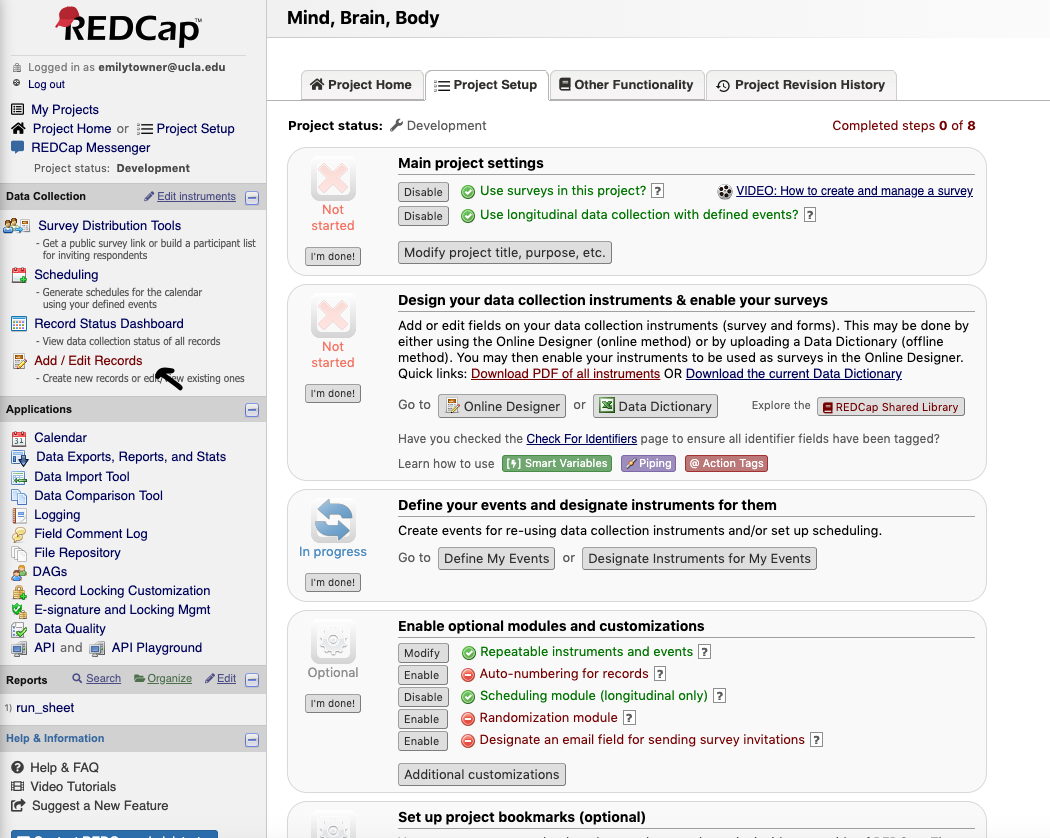
\includegraphics{images/redcap_screening/1.png}
\item
  Click to enter a new Subject ID

  \begin{itemize}
  \tightlist
  \item
    Make sure Arm 1: Recruitment is selected
  \end{itemize}
\item
  Type ``SMBB\#'' (Screener ID) to create a record and hit ``Enter''

  \begin{itemize}
  \tightlist
  \item
    Make sure to link the participants Screener ID and their name on the \textbf{ID Drive ONLY}
  \item
    Before creating a new record, be sure to check the ID Drive to see if the participant already has an existing Screener ID
  \item
    If a record exists, add a new instance of the screen instead of creating a new record
    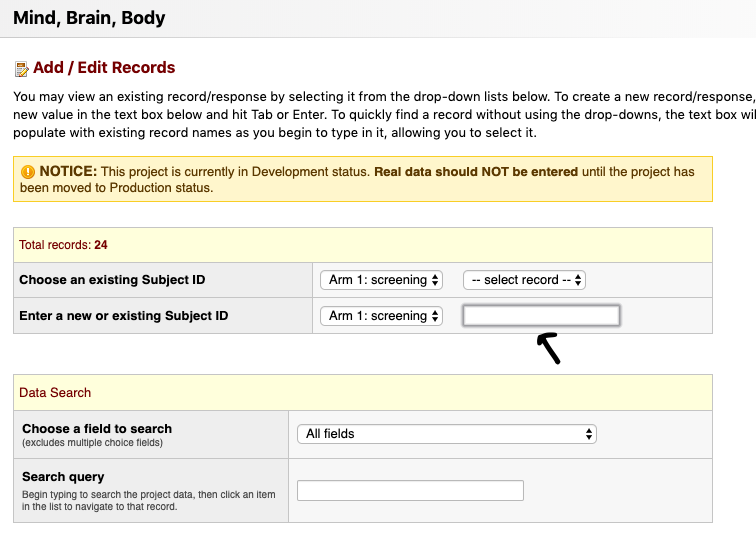
\includegraphics{images/redcap_screening/2.png}
  \end{itemize}
\item
  The screening arm contains two parts

  \begin{itemize}
  \tightlist
  \item
    The screen
  \item
    The wave1\_status

    \begin{itemize}
    \tightlist
    \item
      The wave1\_status is to be updated after the first and each subsequent contact
      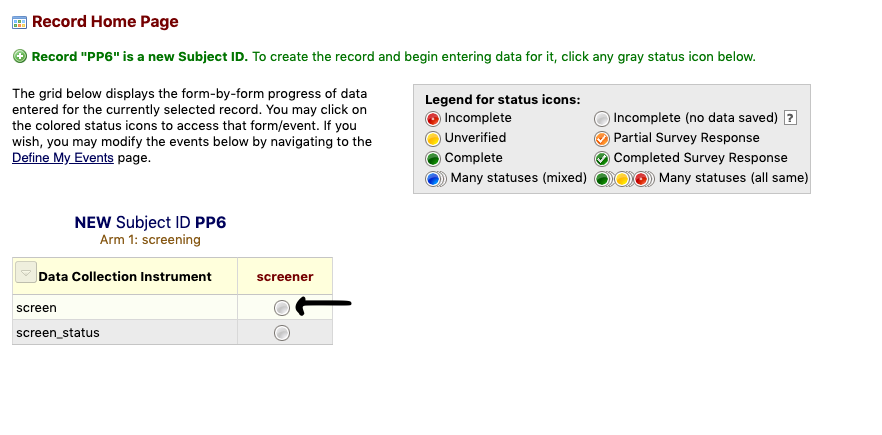
\includegraphics{images/redcap_screening/3.png}
    \end{itemize}
  \end{itemize}
\item
  Click on the radio button in the ``screen'' row to screen the participant
  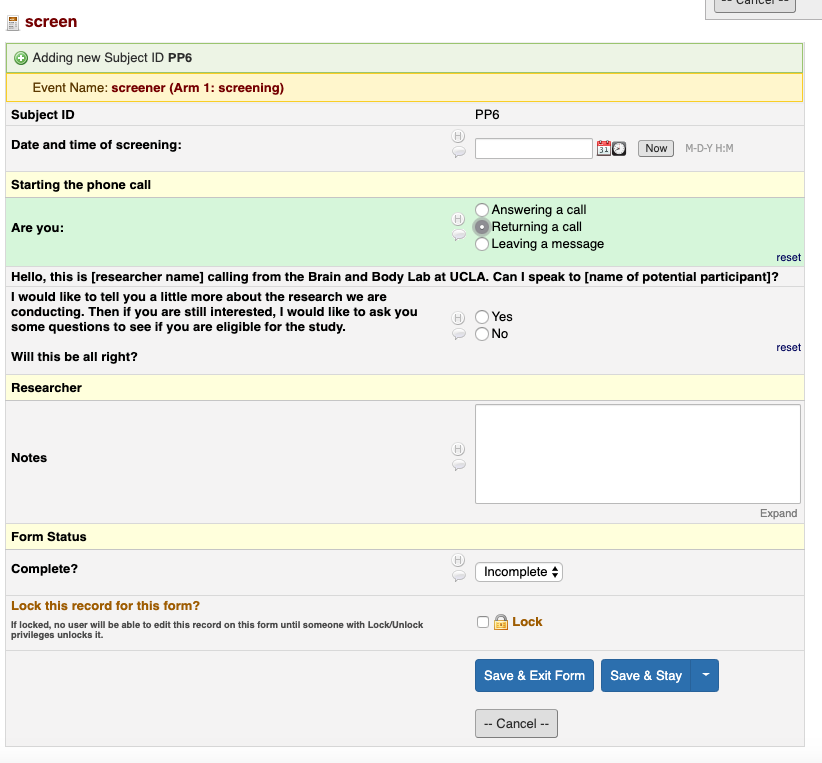
\includegraphics{images/redcap_screening/4.png}
\item
  Click ``Now'' to enter today's date and time
\item
  Select the appropriate choice to start the phone call and follow the skip logic
\item
  Follow the skip logic to the end

  \begin{itemize}
  \tightlist
  \item
    For items without a text field, write the information down in the Recruitment database (This identifying information cannot be on REDCap)
  \end{itemize}
\item
  Once done, select ``Complete'' and ``Save \& Exit Form''

  \begin{itemize}
  \tightlist
  \item
    The screen can be entered multiple times - for instance if there are multiple phone calls or contacts
  \item
    It is important to keep a record of all instances of contact
    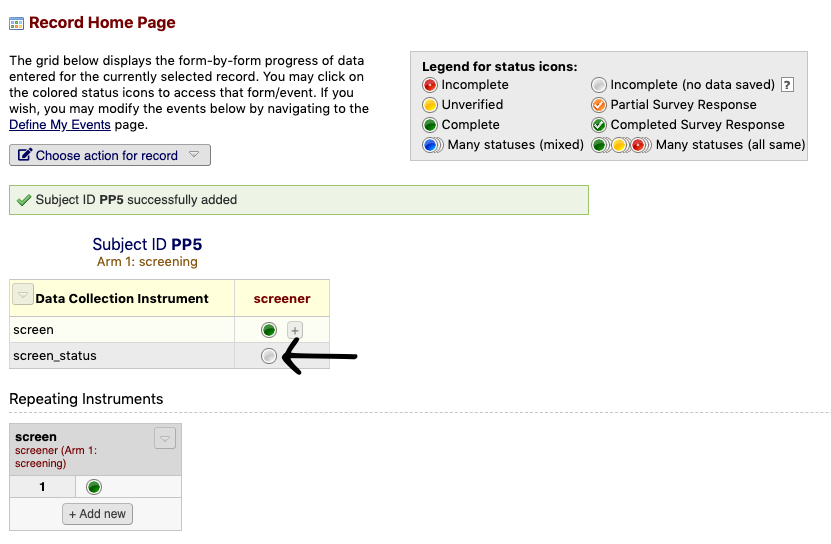
\includegraphics{images/redcap_screening/5.png}
  \end{itemize}
\item
  Click the screen\_status radio button
  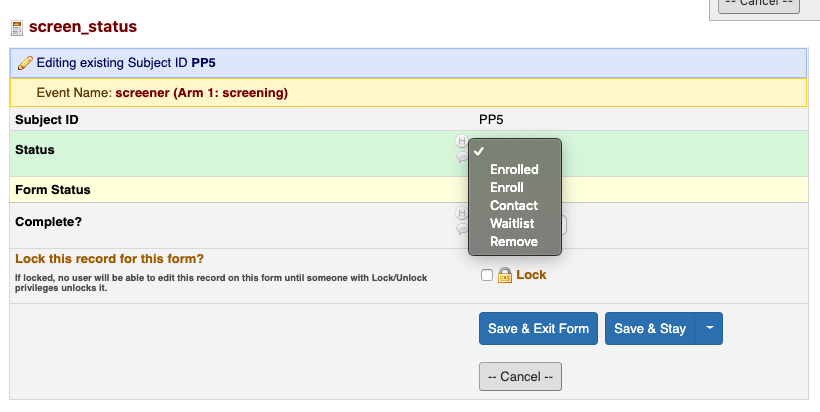
\includegraphics{images/redcap_screening/6.png}
\item
  Select the appropriate option

  \begin{itemize}
  \tightlist
  \item
    Contact - Participant needs to be re-contacted (add Recruitment Database \& ID Drive)
  \item
    Ineligible - Participant not eligible for study
  \item
    To Enroll - Participant to enroll (need to create subject ID, enter subject info, schedule participant, add to Recruitment Database, add to ID Drive)
  \item
    Enrolled - Participant has been enrolled (all above have been completed)
  \item
    To Remove - Participant wants to be removed
  \end{itemize}
\item
  Be sure to update the screen status after each contact

  \begin{itemize}
  \tightlist
  \item
    After 3 contacts (with no response) - review (time of day, contact method, etc.)
  \end{itemize}
\item
  If enrolled, proceed to pre-session checklist in the participant log
\end{enumerate}

\hypertarget{other-screening-information}{%
\subsubsection{Other Screening Information}\label{other-screening-information}}

Accessing Lists

To find out where participants are in the recruitment process, there are several lists.
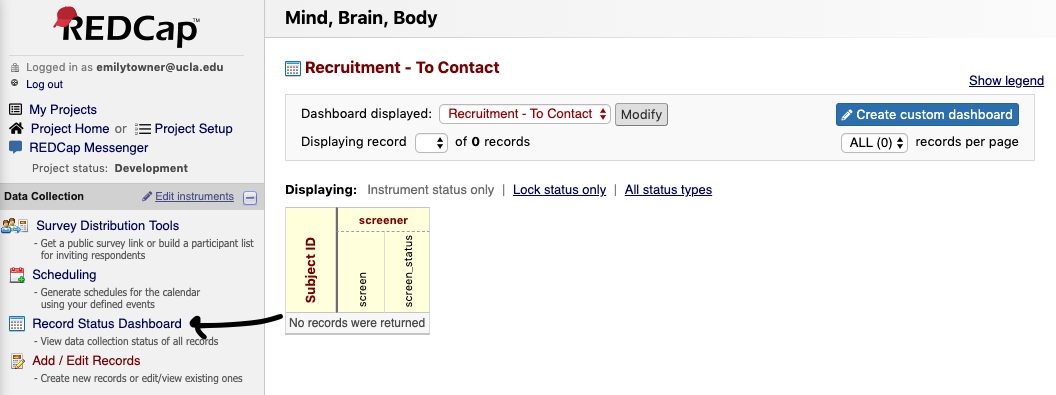
\includegraphics{images/redcap_screening/7.png}
1. Click on ``Record Status Dashboard''
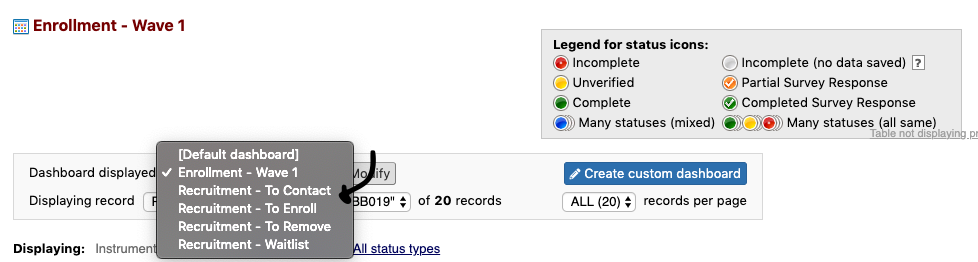
\includegraphics{images/redcap_screening/8.png}
2. Participants who have been enrolled will be listed in the Enrollment - Wave 1 list
3. Participants in the process of recruitment will be listed in one of the 4 Recruitment lists
- *These lists are populated based on the individuals ``Screen Status'' so be sure to update after each contact!

List Types

\begin{itemize}
\tightlist
\item
  Contact - List of individuals who need to be contacted or re-contacted (also includes waitlist)
\item
  Ineligible - Participants are ineligible but interested
\item
  To Enroll - Participants who have been screened and are eligible to enroll
\item
  To Remove - Participants who were not interested in being contacted for this or future research
\end{itemize}

\begin{center}\rule{0.5\linewidth}{0.5pt}\end{center}

\hypertarget{addressing-concerns}{%
\subsection{Addressing Concerns}\label{addressing-concerns}}

If a parent has a concern about the study before the session, send the email template:

\begin{itemize}
\tightlist
\item
  {[}MBB - CONCERNS{]}
\end{itemize}

\begin{center}\rule{0.5\linewidth}{0.5pt}\end{center}

\hypertarget{parentchild-observation}{%
\subsection{Parent/Child Observation}\label{parentchild-observation}}

The parent and child will be in the Rainbow Room for 15 minutes. During that time they will be filmed while planning a conflict event, and then again while discussing a pleasant event. The conflict event will always go first, followed by the pleasant event. We did this to ensure that the parents were not thinking of the negative interaction upon answering the questionnaires about their child, which they did immediately after the observation interaction. If participants indicate that they prefer to speak in a language other than English, they may do so.

\textbf{Step 1}:

Parent and child will be situated on the grey couch in the Rainbow Room. The iPad video camera will be placed about 4 feet away from the dyad, on a tripod stand. The screen of the iPad will be facing away from the parent and child.

\begin{figure}
\centering
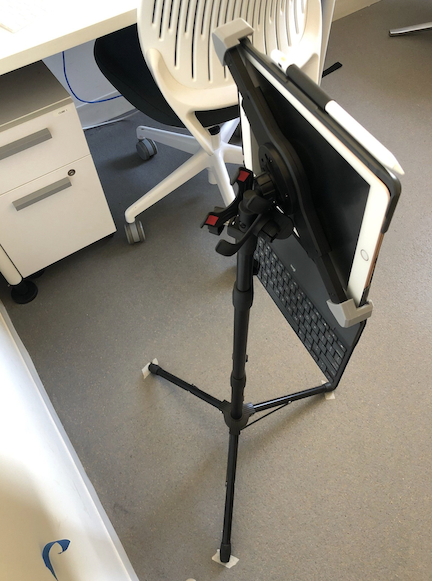
\includegraphics{images/parent:child_obser/2.png}
\caption{}
\end{figure}

\textbf{Step 2}:

The researcher will give the parent and child the Pleasant Events Checklist (PEC) on a piece of paper.

\emph{Researcher: Next we are going to take some film of you while you discuss a source of conflict (or something you disagree on) and try to resolve it. On this piece of paper is a list of things that parents and children sometimes have disagreements about. Please take a moment to read the list and think about some that you would like to discuss together. When I knock on the door, please start discussing the things you have selected from the list and try to resolve the areas of conflict you have chosen from the list. You do not need to tell us what you chose to discuss, and it does not matter if you chose something from the list, or decide to choose something else not included on the list. I will give you five minutes to discuss the event, then I will come back and give you further instructions.}

\textbf{Step 3}:

Researcher press record on the iPad and leave the room. Start timer for 1 minute, then knock on the door and ask the dyad to begin discussing their event. Start timer for 5 minutes. At the end of 5 minutes, again knock on the door and enter the Rainbow Room.

\emph{Researcher: Thank you for taking the time to discuss the source of conflict and try to resolve it. Next we are going to take some film of you while you discuss a pleasant event you could do together. On this piece of paper is a list of events that parents and children sometimes find pleasant to do together. Please take a moment to read the list of events and think about what you would like to plan to do together. When I knock on the door, please start discussing the event you would like to do together and make a plan for how you could do it. You do not need to tell us what you chose to discuss, and it does not matter if you chose something from the list, or decide to choose something else not included on the list. I will give you five minutes to discuss the event, then I will come back and give you further instructions.}

\textbf{Step 4}:

Researcher press record on the iPad and leave the room. Start timer for 1 minute, then knock on the door and ask the dyad to begin discussing their event. Start timer for 5 minutes. At the end of 5 minutes, again knock on the door and enter the Rainbow Room.

\textbf{Step 5}:

Researcher reenter the room, switch the iPad off and move the child/adolescent to their next session.

\begin{longtable}[]{@{}ll@{}}
\toprule
\begin{minipage}[b]{0.50\columnwidth}\raggedright
Pleasant Events Checklist\strut
\end{minipage} & \begin{minipage}[b]{0.44\columnwidth}\raggedright
Issues Checklist\strut
\end{minipage}\tabularnewline
\midrule
\endhead
\begin{minipage}[t]{0.50\columnwidth}\raggedright
Being in the country\strut
\end{minipage} & \begin{minipage}[t]{0.44\columnwidth}\raggedright
Telephone calls\strut
\end{minipage}\tabularnewline
\begin{minipage}[t]{0.50\columnwidth}\raggedright
Talking about sports\strut
\end{minipage} & \begin{minipage}[t]{0.44\columnwidth}\raggedright
Bedtime\strut
\end{minipage}\tabularnewline
\begin{minipage}[t]{0.50\columnwidth}\raggedright
Going to a concert\strut
\end{minipage} & \begin{minipage}[t]{0.44\columnwidth}\raggedright
Cleaning bedroom\strut
\end{minipage}\tabularnewline
\begin{minipage}[t]{0.50\columnwidth}\raggedright
Planning trips or vacations\strut
\end{minipage} & \begin{minipage}[t]{0.44\columnwidth}\raggedright
Doing homework\strut
\end{minipage}\tabularnewline
\begin{minipage}[t]{0.50\columnwidth}\raggedright
Being at the beach\strut
\end{minipage} & \begin{minipage}[t]{0.44\columnwidth}\raggedright
Putting away clothes\strut
\end{minipage}\tabularnewline
\begin{minipage}[t]{0.50\columnwidth}\raggedright
Doing art work (painting, sculpture, drawing, movie-making)\strut
\end{minipage} & \begin{minipage}[t]{0.44\columnwidth}\raggedright
Using the television\strut
\end{minipage}\tabularnewline
\begin{minipage}[t]{0.50\columnwidth}\raggedright
Rock climbing or mountaineering\strut
\end{minipage} & \begin{minipage}[t]{0.44\columnwidth}\raggedright
Cleanliness (washing, showers, brushing teeth)\strut
\end{minipage}\tabularnewline
\begin{minipage}[t]{0.50\columnwidth}\raggedright
Playing golf\strut
\end{minipage} & \begin{minipage}[t]{0.44\columnwidth}\raggedright
Which clothes to wear\strut
\end{minipage}\tabularnewline
\begin{minipage}[t]{0.50\columnwidth}\raggedright
Re-arranging or redecorating my room or house\strut
\end{minipage} & \begin{minipage}[t]{0.44\columnwidth}\raggedright
How neat clothes look\strut
\end{minipage}\tabularnewline
\begin{minipage}[t]{0.50\columnwidth}\raggedright
Going to a sports event\strut
\end{minipage} & \begin{minipage}[t]{0.44\columnwidth}\raggedright
Making too much noise at home\strut
\end{minipage}\tabularnewline
\begin{minipage}[t]{0.50\columnwidth}\raggedright
Reading stories, novels, poems, or plays\strut
\end{minipage} & \begin{minipage}[t]{0.44\columnwidth}\raggedright
Table manners\strut
\end{minipage}\tabularnewline
\begin{minipage}[t]{0.50\columnwidth}\raggedright
Making music together\strut
\end{minipage} & \begin{minipage}[t]{0.44\columnwidth}\raggedright
Fighting with siblings (brothers and sisters)\strut
\end{minipage}\tabularnewline
\begin{minipage}[t]{0.50\columnwidth}\raggedright
Boating (canoeing, kyaking, motorboating, sailing, etc\strut
\end{minipage} & \begin{minipage}[t]{0.44\columnwidth}\raggedright
Cursing\strut
\end{minipage}\tabularnewline
\begin{minipage}[t]{0.50\columnwidth}\raggedright
Watching TV\strut
\end{minipage} & \begin{minipage}[t]{0.44\columnwidth}\raggedright
How money is spent\strut
\end{minipage}\tabularnewline
\begin{minipage}[t]{0.50\columnwidth}\raggedright
Camping\strut
\end{minipage} & \begin{minipage}[t]{0.44\columnwidth}\raggedright
Picking books or movies\strut
\end{minipage}\tabularnewline
\begin{minipage}[t]{0.50\columnwidth}\raggedright
Playing cards\strut
\end{minipage} & \begin{minipage}[t]{0.44\columnwidth}\raggedright
Allowance\strut
\end{minipage}\tabularnewline
\begin{minipage}[t]{0.50\columnwidth}\raggedright
Completing a difficult task\strut
\end{minipage} & \begin{minipage}[t]{0.44\columnwidth}\raggedright
Going places without parents (shopping, movies, etc)\strut
\end{minipage}\tabularnewline
\begin{minipage}[t]{0.50\columnwidth}\raggedright
Laughing\strut
\end{minipage} & \begin{minipage}[t]{0.44\columnwidth}\raggedright
Playing stereo or radio too loudly\strut
\end{minipage}\tabularnewline
\begin{minipage}[t]{0.50\columnwidth}\raggedright
Solving a problem, puzzle, crossword\strut
\end{minipage} & \begin{minipage}[t]{0.44\columnwidth}\raggedright
Turning off lights in house\strut
\end{minipage}\tabularnewline
\begin{minipage}[t]{0.50\columnwidth}\raggedright
Playing tennis\strut
\end{minipage} & \begin{minipage}[t]{0.44\columnwidth}\raggedright
Taking care of records, games\strut
\end{minipage}\tabularnewline
\begin{minipage}[t]{0.50\columnwidth}\raggedright
Driving long distances\strut
\end{minipage} & \begin{minipage}[t]{0.44\columnwidth}\raggedright
Buying records, games, toys, and other things\strut
\end{minipage}\tabularnewline
\begin{minipage}[t]{0.50\columnwidth}\raggedright
Woodworking, carpentry\strut
\end{minipage} & \begin{minipage}[t]{0.44\columnwidth}\raggedright
Going on dates\strut
\end{minipage}\tabularnewline
\begin{minipage}[t]{0.50\columnwidth}\raggedright
Writing stones, novels, plays or poetry\strut
\end{minipage} & \begin{minipage}[t]{0.44\columnwidth}\raggedright
Who friends should be\strut
\end{minipage}\tabularnewline
\begin{minipage}[t]{0.50\columnwidth}\raggedright
Being with animals\strut
\end{minipage} & \begin{minipage}[t]{0.44\columnwidth}\raggedright
Selecting new clothes\strut
\end{minipage}\tabularnewline
\begin{minipage}[t]{0.50\columnwidth}\raggedright
Riding in an airplane\strut
\end{minipage} & \begin{minipage}[t]{0.44\columnwidth}\raggedright
Coming home on time\strut
\end{minipage}\tabularnewline
\begin{minipage}[t]{0.50\columnwidth}\raggedright
Exploring (hiking away from known routes)\strut
\end{minipage} & \begin{minipage}[t]{0.44\columnwidth}\raggedright
Getting to school on time\strut
\end{minipage}\tabularnewline
\begin{minipage}[t]{0.50\columnwidth}\raggedright
Going to a party\strut
\end{minipage} & \begin{minipage}[t]{0.44\columnwidth}\raggedright
Getting low grades in school\strut
\end{minipage}\tabularnewline
\begin{minipage}[t]{0.50\columnwidth}\raggedright
Playing a musical instrument\strut
\end{minipage} & \begin{minipage}[t]{0.44\columnwidth}\raggedright
Getting in trouble at school\strut
\end{minipage}\tabularnewline
\begin{minipage}[t]{0.50\columnwidth}\raggedright
Making snacks\strut
\end{minipage} & \begin{minipage}[t]{0.44\columnwidth}\raggedright
Lying\strut
\end{minipage}\tabularnewline
\begin{minipage}[t]{0.50\columnwidth}\raggedright
Snow skiing\strut
\end{minipage} & \begin{minipage}[t]{0.44\columnwidth}\raggedright
Helping out around the house\strut
\end{minipage}\tabularnewline
\begin{minipage}[t]{0.50\columnwidth}\raggedright
Doing craft work (pottery, jewelry, leather, beads, weaving, etc)\strut
\end{minipage} & \begin{minipage}[t]{0.44\columnwidth}\raggedright
Talking back to parents\strut
\end{minipage}\tabularnewline
\begin{minipage}[t]{0.50\columnwidth}\raggedright
\strut
\end{minipage} & \begin{minipage}[t]{0.44\columnwidth}\raggedright
Getting up in the morning\strut
\end{minipage}\tabularnewline
\begin{minipage}[t]{0.50\columnwidth}\raggedright
\strut
\end{minipage} & \begin{minipage}[t]{0.44\columnwidth}\raggedright
Bothering parents when they want to be left alone\strut
\end{minipage}\tabularnewline
\begin{minipage}[t]{0.50\columnwidth}\raggedright
\strut
\end{minipage} & \begin{minipage}[t]{0.44\columnwidth}\raggedright
Bothering child/adolescent when they want to be left alone\strut
\end{minipage}\tabularnewline
\begin{minipage}[t]{0.50\columnwidth}\raggedright
\strut
\end{minipage} & \begin{minipage}[t]{0.44\columnwidth}\raggedright
Putting feet on furniture\strut
\end{minipage}\tabularnewline
\begin{minipage}[t]{0.50\columnwidth}\raggedright
\strut
\end{minipage} & \begin{minipage}[t]{0.44\columnwidth}\raggedright
Messing up the house\strut
\end{minipage}\tabularnewline
\begin{minipage}[t]{0.50\columnwidth}\raggedright
\strut
\end{minipage} & \begin{minipage}[t]{0.44\columnwidth}\raggedright
What time to have meals\strut
\end{minipage}\tabularnewline
\begin{minipage}[t]{0.50\columnwidth}\raggedright
\strut
\end{minipage} & \begin{minipage}[t]{0.44\columnwidth}\raggedright
How to spend free time\strut
\end{minipage}\tabularnewline
\begin{minipage}[t]{0.50\columnwidth}\raggedright
\strut
\end{minipage} & \begin{minipage}[t]{0.44\columnwidth}\raggedright
Earning money away from the house\strut
\end{minipage}\tabularnewline
\begin{minipage}[t]{0.50\columnwidth}\raggedright
\strut
\end{minipage} & \begin{minipage}[t]{0.44\columnwidth}\raggedright
What child/adolescent eats\strut
\end{minipage}\tabularnewline
\bottomrule
\end{longtable}

\hypertarget{coding-the-interview}{%
\subsubsection{Coding the Interview}\label{coding-the-interview}}

\begin{itemize}
\item
  After the interviews are collected, videos will be coded by two observers blind to the caregiving group of the child (adversity or comparison).
\item
  Our original plan was to follow the LIFE coding system developed by Hops:

  \begin{itemize}
  \tightlist
  \item
    Hops H, Davis B, Longoria N. Methodological issues in direct observation -- Illustrations with the Living in Familial Environments (LIFE) coding system. Journal of Clinical Child Psychology. 1995;24:193--203. \href{https://www.tandfonline.com/doi/abs/10.1207/s15374424jccp2402_7?journalCode=hcap19}{Google Scholar}
  \end{itemize}
\item
  However, this system is prohibitively expensive and very training intensive. Instead we decided to go with either of the following two coding schedules:

  \begin{itemize}
  \item
    \begin{enumerate}
    \def\labelenumi{\arabic{enumi}.}
    \tightlist
    \item
      Family Interaction Macrocoding Schedule (FIMS) Holmbeck, Zebracki, Johnson, Belvedere, \& Hommeyer, 2007.
    \end{enumerate}
  \item
    \begin{enumerate}
    \def\labelenumi{\arabic{enumi}.}
    \setcounter{enumi}{1}
    \tightlist
    \item
      CIB Training with Ruth Feldman.
    \end{enumerate}
  \end{itemize}
\item
  We ultimately decided to go with FIMS for several reasons:

  \begin{itemize}
  \tightlist
  \item
    Expense - Sarah Whittle paid approximately \$ 1000USD for a 10 hour skype training session with one of Holmbeck's team), whereas CIB training is /\$2500 and also involves flights and accommodation at Yale.
  \item
    Validation in age range - I like CIB for younger children, but FIMS was designed for older children and adolescents, and Sarah Whittle has validated it in a community sample of 8 year olds and their mothers.
  \item
    FIMS is a less intensive coding schedule, producing global codes, rather than micro coded (i.e., minute to minute) scales - which makes more intuitive sense in the age range for MBB.
  \item
    FIMS has a peer version that we might brach out to in the future (but likely not needing further training): \url{https://psycnet.apa.org/record/2014-24011-001}
  \item
    Sarah Whittle's group looked at the component structure for the FIMS and found components that seemed close to what they were finding with the Hops LIFE system - namely: negative maternal affect during pleasant event, negative maternal during conflict discussion, and pleasant maternal affect across both tasks (warmth). The negative maternal during pleasant event was the most predictive of child behavior problems. Overall, the correlations they report in their paper are all very sensical and convinced me that we should use the FIMS. \url{https://journals.sagepub.com/doi/full/10.1177/1073191118796557}
  \end{itemize}
\end{itemize}

\hypertarget{childteen-protocols}{%
\section{Child/Teen Protocols}\label{childteen-protocols}}

\begin{center}\rule{0.5\linewidth}{0.5pt}\end{center}

\hypertarget{biopac-electrode-hookup}{%
\subsection{BioPac Electrode Hookup}\label{biopac-electrode-hookup}}

\hypertarget{electrode-placementpreparation}{%
\subsubsection{Electrode Placement/Preparation}\label{electrode-placementpreparation}}

\begin{itemize}
\tightlist
\item
  Wheel the cart into the Rainbow Room
\item
  Prep 2 electrodes with Gel 101. Stick to the participant's ring and middle fingers on their non-dominant hand (we want to keep the pointer finger free so they can use it for tasks)
\item
  Wrap medical tape around these to secure them, but ensure that the metal poles are still accessible
\item
  Look at the skeleton diagram and use the EL-PREP Gel to abrade the skin around the remaining electrode sites (below the collarbones, below the sternum, on the left lower ribs, and in the remaining two positions on the stomach and left ribs)
\item
  Clean the remaining EL-PREP off with a tissue or baby wipe
\item
  Prep 8 electrodes with Gel 100. Stick to the locations indicated on the skeleton diagram
\item
  Let all electrodes sit for the duration of the interaction filming task
\end{itemize}

\hypertarget{gsr}{%
\subsubsection{GSR}\label{gsr}}

\begin{itemize}
\tightlist
\item
  Put on gloves
\item
  Ensure that the finger electrodes are properly adhered and have had time to rest
\item
  Make sure the lead wire module is connected to the transmitter (PPGED, blue sticker) in the ``EDA'' channel
\item
  Take the transmitter and secure it around the participant's wrist as shown below
\item
  Hook up the lead wires so that the black wire connects to the middle finger and the red wire connects to the ring finger
\item
  Ask the participant to wear a glove over the whole setup to secure it throughout the tasks
\item
  To check if the GSR is working properly, ask the participant to briefly hold his/her breath - you should see a rise in the signal on the graph
\end{itemize}

\hypertarget{ecg}{%
\subsubsection{ECG}\label{ecg}}

\begin{itemize}
\tightlist
\item
  Ensure that the chest electrodes are properly adhered and have had time to rest.
\item
  Make sure the lead wire module is connected to the transmitter (RSPEC-R, yellow sticker) in the ECG channel.
\item
  Take the transmitter and secure it around the participant's stomach as shown below.
\item
  Hook up the lead wires so that the white lead connects to the Right Collarbone electrode, the black lead connects to the Left Collarbone electrode, and the red lead connects to the lowest Left Rib electrode.
\end{itemize}

\hypertarget{egg}{%
\subsubsection{EGG}\label{egg}}

\begin{itemize}
\tightlist
\item
  Ensure that the chest electrodes are properly adhered and have had time to rest.
\item
  Make sure the lead wires are connected to the transmitter (EGG2-R, red sticker). The lead module labelled ``A'' (3 short leads) should be in the EGG A channel, while the lead module labelled ``B'' (2 long leads) should be in the EGG B channel.
\item
  Take the transmitter and secure it around the participant's stomach as show below.
\item
  Hook up the lead wires so that the ``A'' and ``B'' channel white leads connect to the sternum electrodes (which goes to which does not matter), the ``A'' and ``B'' channel red leads connects to the upper left rib electrode and stomach electrode, and the ``B'' channel black lead connects to the remaining lower left rib electrode.
\end{itemize}

\hypertarget{acqknowledge}{%
\subsubsection{AcqKnowledge}\label{acqknowledge}}

\begin{itemize}
\tightlist
\item
  Turn off the wifi on the Mac Mini and turn on the BioPac/transmitters
\item
  Open AcqKnowledge
\item
  Choose the graph template file
\item
  Once it loads, make sure all of the transmitters are connected
\item
  Press run and click through all of the dialog boxes that are generated
\end{itemize}

\begin{center}\rule{0.5\linewidth}{0.5pt}\end{center}

\hypertarget{memory-intrusionmovie-watching}{%
\subsection{Memory Intrusion/Movie Watching}\label{memory-intrusionmovie-watching}}

\begin{itemize}
\item
  There are 4 counterbalanced versions of this task:

  \begin{itemize}
  \tightlist
  \item
    DRM\_A\_incongruent\_first.psyexp
  \item
    DRM\_A\_congruent\_first.psyexp
  \item
    DRM\_B\_congruent\_first.psyexp
  \item
    DRM\_B\_incongruent\_first.psyexp
  \end{itemize}
\item
  Choose the counterbalanced version that is correct for the participant
\item
  First open the task, add the participant ID number and press start
\item
  Read the instructions to the participant:

  \emph{Welcome to the movie game. First you will watch some movies. Then you will hear a list of words. Try to remember the words on the list.}
\item
  Press the space bar to progress to the next screen and read the instructions:

  \emph{Get ready, to watch the movie. Turn to the laptop to watch.}
\item
  Open up the first movie for the participant. It will depend on the counterbalancing condition what movie goes first.
\item
  For the two files that start with ``DRM\_A'':

  \begin{itemize}
  \tightlist
  \item
    DRM\_A\_congruent\_first.psyexp
  \item
    DRM\_A\_incongruent\_first.psyexp
  \end{itemize}
\end{itemize}

\textbf{The order will be: Sad --\textgreater{} Neutral --\textgreater{} Scary}

\begin{itemize}
\tightlist
\item
  For the two files that start with ``DRM\_B'':

  \begin{itemize}
  \tightlist
  \item
    DRM\_B\_congruent\_first.psyexp
  \item
    DRM\_B\_incongruent\_first.psyexp
  \end{itemize}
\end{itemize}

\textbf{The order will be: Scary --\textgreater{} Neutral --\textgreater{} Sad}

\begin{itemize}
\item
  Simultaneously press play on the movie on the laptop while also pressing the spacebar on the psychopy task. This will start the physiology and the movie at about the same time. While the movie is playing there will be a box of popcorn on the computer screen.
\item
  When the movie is done, press spacebar on the psychopy computer to progress to the next screen. Read the instructions for the participant:
\item
  Click on the face that shows how you feel after watching the movies.
\item
  Participants can use a mouse to click on the face that matches the way they feel after watching the movie. The faces range in valence (negative to positive) across the X axis, and arousal (low to high) up the Y axis.
\item
  After the participant has selected a face, you will be taken to the next screen where you can read the instructions for the participants:

  \emph{Listen to the list of words and try to remember all of them.}
\item
  When the participant indicates that they have understood the instructions, press the spacebar and progress to the next screen. Make sure that the computer volume is up and the participant can hear the words being pronounced on the computer screen. After the participant hears all the words the distractor task will start.
\item
  Read the distractor task instructions to the participant:

  \emph{Count backwards from the number 25 out loud for the researcher.}
\end{itemize}

\textbf{Note: Whether the participant completes the distractor task correctly or not doesn't matter. The only purpose of the distractor task is to distract the participant for a brief period of time. Listen while they count backwards. If they can't count backwards, ask them to count forwards.}

\begin{itemize}
\item
  When the participant is finished counting backwards from 25, or after approximately 30s has passed (whatever comes first), progress to the next screen by pressing the spacebar.
\item
  Read the instructions out loud to the participant:

  \emph{Recall 1. Please tell the researcher all the words that you can remember from the list.}
\item
  Before the participant starts to tell you what they remember, start a new voice recording and then tell them to start while you record what they say (on the talk setting). Also write what they say on a piece of paper. Make sure to note that this is `Recall 1' (as there is a second recall later on). When the participant has told you all the words they can remember, or after 60s, progress to the next screen (instructions for the next word list).
\item
  Make one recording for all of the memory intrusion task
\item
  Read the instructions aloud for the participant.

  \emph{Now you will hear another word list. Get ready!}
\item
  Press the spacebar to hear the word list. After the word list, move to the distractor task (counting backwards from 25). After the distractor task, move to the second recall task and record the participant like the first. When the second recall task is complete, a new loop will begin. Read the instructions to the participant then start the next movie (which will always be neutral). Repeat everything again for the final loop after they watch the final movie, which will either be sad or scary.
\item
  Physiology Marks:

  \begin{itemize}
  \tightlist
  \item
    We have inserted start and stop times for the physiology for the movie component of the task, which will be used for one of the analyses. We have also inserted physiology marks for the start and stop times for each of the word lists, and finally for the recall phases. Note: be careful using physiology during the recall phase, as the participant is talking during that phase.
  \end{itemize}
\end{itemize}

\begin{center}\rule{0.5\linewidth}{0.5pt}\end{center}

\hypertarget{halloween}{%
\subsection{Halloween}\label{halloween}}

\begin{itemize}
\item
  Check master counterbalance sheet and fill out the participant's ID \# in the group which you assigned them.
\item
  Seat the participant at the computer desk in the Bear's Den. Close the door to ensure privacy and freedom from distractions.
\item
  Set up the task:

  \begin{itemize}
  \item
    \begin{enumerate}
    \def\labelenumi{\alph{enumi}.}
    \tightlist
    \item
      Navigate through the Finder to get to the task following this path:
      Dropbox/BAB/Studies/Mind\_Brain\_Body/Tasks/Wave1/04\_halloween\_pilot
      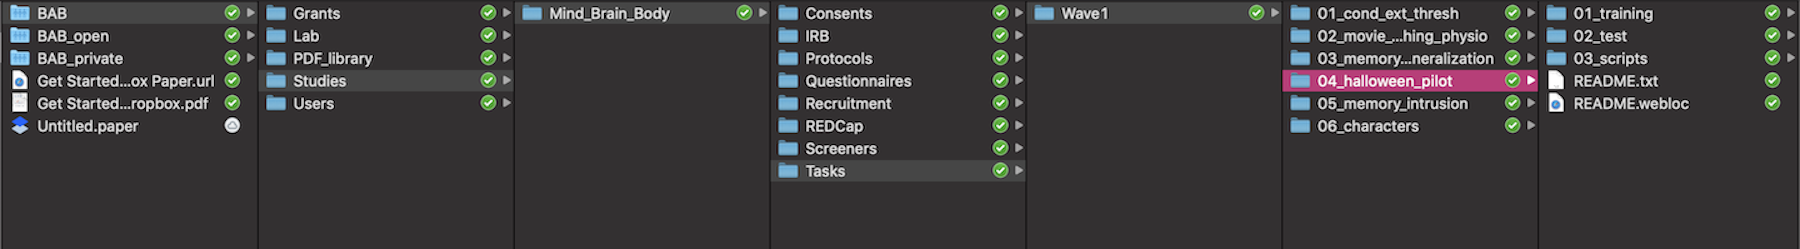
\includegraphics{images/halloween/1.png}
    \end{enumerate}
  \item
    \begin{enumerate}
    \def\labelenumi{\alph{enumi}.}
    \setcounter{enumi}{1}
    \item
      Start by going into the folder titled ``01\_training'' and selecting ``Halloween\_training\_day1.psyexp'' if the participant is in the ``day first'' group or ``Halloween\_training\_night1.psyexp'' if the participant is in the ``night first'' group.

      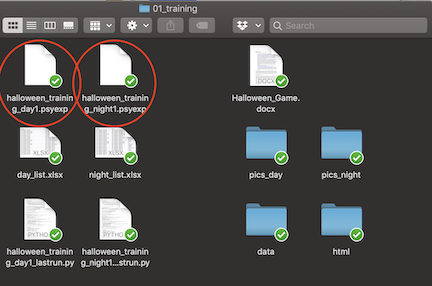
\includegraphics{images/halloween/2.png}
    \end{enumerate}
  \end{itemize}
\item
  When the task pulls up and the participant is situated and ready, select the run button indicated below:

  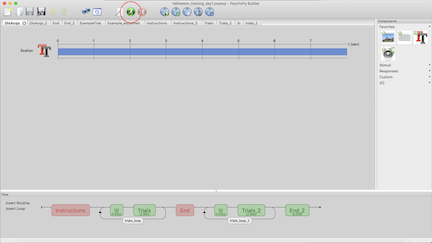
\includegraphics{images/halloween/3.png}
\item
  When prompted, fill in the participant's ID \# in the ``participant'' field:
  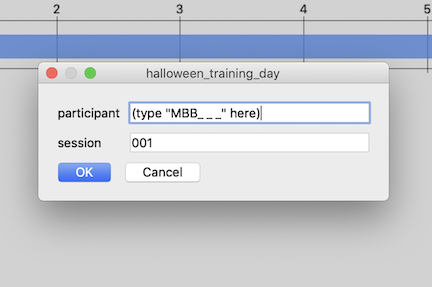
\includegraphics{images/halloween/4.png}
\item
  Guide the participant through the instructional slides by pressing the space bar every time {[}s{]} shows up on the screen. Make sure to remind the participant to read all of the instructions carefully.
\item
  Once the training task starts, sit quietly and do not disturb the participant. It is important for them to pay their undivided attention to the images on screen during the training.
\item
  When the break slide appears, ask them to let you know when they are ready to continue. Press the space bar to proceed on to the next set of images.
\item
  Once the task is complete, you can exit out by pressing any key and then closing the the PsychoPy file.
\item
  Prompt the testing phase of the exercise by saying something along the lines of:
  \emph{``And now we want to see how much of your trick-or-treating adventure you remember.''}
\item
  Go into the ``02\_test'' file and select the ``Halloween\_day1.psyexp'' file if the participant is in the ``day first'' group or ``Halloween\_night1.psyexp'' if the participant is in the ``night first'' group.
  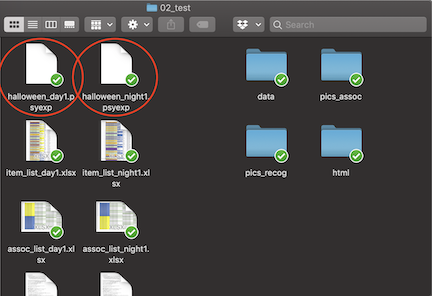
\includegraphics{images/halloween/5.png}
\item
  When the task pulls up and the participant is situated and ready, select the run button indicated below:

  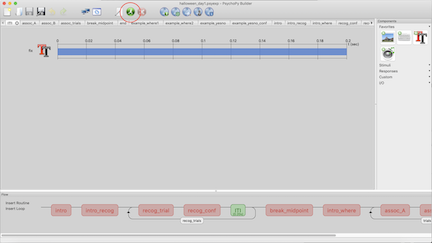
\includegraphics{images/halloween/6.png}
\item
  Guide the participant through the instructional slides by pressing the space bar every time {[}s{]} shows up on the screen. Make sure to remind the participant to read all of the instructions carefully. Remind them that they need to click the words for the answer they want to provide.
\item
  When the break slide appears, ask them to let you know when they are ready to continue. Press the space bar to proceed on to the next tests.
\item
  Guide the participant through the instructional slides by pressing the space bar every time {[}s{]} shows up on the screen. Make sure to remind the participant to read all of the instructions carefully. Remind them that they need to click the item for the answer they want to provide, and then click which quadrant of the scene image they want to pick.
\item
  Once the task is complete, you can exit out by pressing any key and then closing the the PsychoPy file.
\item
  Data is saved automatically in the data folder. You do not need to save anything before exiting out of the psychopy folder
\end{itemize}

\emph{Troubleshooting:}

If the task exits due to an error, take a screenshot of the error screen and message Emily, Kristen, or Bridget for assistance. Move onto the next task in the meantime.

\begin{center}\rule{0.5\linewidth}{0.5pt}\end{center}

\hypertarget{disccondext}{%
\subsection{Disc/Cond/Ext}\label{disccondext}}

\hypertarget{discrimination}{%
\subsubsection{Discrimination}\label{discrimination}}

\begin{itemize}
\tightlist
\item
  Click into the discrimination folder
\item
  Right click on either discrimination\_horiz.py or discrimination\_vert.py (depending on counterbalancing) and open in PsychoPy

  \begin{itemize}
  \tightlist
  \item
    This task was not created in Builder view, so does not have a .psyexp file.
  \end{itemize}
\item
  Click the green running man and enter the Participant ID

  \begin{itemize}
  \tightlist
  \item
    Make sure to enter the correct run number
  \item
    Discrimination will be repeated 3 times (run 1, run 2, and run 3)
  \end{itemize}
\item
  Move the keyboard over so that the you, the researcher, can control it

  \begin{itemize}
  \tightlist
  \item
    You will press the buttons for the participant in this task (it is difficult to do and pay attention to on one's own)
  \end{itemize}
\item
  Read the instructions for the participant
\item
  Ask the participant to tell you which line was more tilted, the first or second and press the corresponding button for them
\end{itemize}

\hypertarget{conditioning}{%
\subsubsection{Conditioning}\label{conditioning}}

\begin{itemize}
\tightlist
\item
  Click into the conditioning folder

  \begin{itemize}
  \tightlist
  \item
    Test the sound file on the laptop - screech.ogg
  \item
    Set so that the sound is loud and uncomfortable, but not hurting
  \item
    Record the volume setting on the session checklist
  \end{itemize}
\item
  Open the .psyexp file for the appropriate counterbalance by right clicking and opening in PsychoPy
\item
  Click the green running man icon and enter the Participant ID
\end{itemize}

\hypertarget{extinction}{%
\subsubsection{Extinction}\label{extinction}}

\begin{itemize}
\tightlist
\item
  Click into the extinction folder
\item
  Open the .psyexp file
\item
  Click the green running man icon and enter the Participant ID
\end{itemize}

\begin{center}\rule{0.5\linewidth}{0.5pt}\end{center}

\hypertarget{height}{%
\subsection{Height}\label{height}}

\begin{itemize}
\tightlist
\item
  Place participant directly against wall/frame
\item
  Advise participant to stand up straight
\item
  Make sure heels of participant are up against the wall/frame
\item
  Use a flat object (booklet, ruler, sheet of paper, etc.) to accurately measure height in inches
\item
  Record height on Lab Session Checklist
\end{itemize}

\begin{center}\rule{0.5\linewidth}{0.5pt}\end{center}

\hypertarget{hair-sample}{%
\subsection{Hair Sample}\label{hair-sample}}

\hypertarget{set-up-hair-sample-station}{%
\subsubsection{Set Up Hair-Sample Station}\label{set-up-hair-sample-station}}

\begin{itemize}
\tightlist
\item
  Ensure the hair-sample station is set up accordingly:

  \begin{itemize}
  \tightlist
  \item
    1 sheet of aluminum foil
  \item
    1 small ziplock bag with participant ID
  \item
    1 salon grade scissor
  \item
    1 wide and narrow tooth parting comb
  \item
    1 alcohol swab
  \item
    Painter-tape
  \item
    1 permanent marker
  \item
    1 pair of gloves
  \item
    2 alligator curl clips
  \item
    1 hair claw clip (for long hair)
  \item
    1 printed copy of the \href{https://app.box.com/file/630323877918}{Hair-Care Practice Questionnaire}
  \item
    Sample hair amount taken from wig
  \end{itemize}
\end{itemize}

\hypertarget{prior-to-getting-hair-sample}{%
\subsubsection{Prior to Getting Hair Sample}\label{prior-to-getting-hair-sample}}

\begin{itemize}
\tightlist
\item
  With the parent present in the room, explain to both the child and parent that we will be collecting 30-50 strands of hair. The amount of hair to be collected is less hair than is lost in normal everyday-brushing from the back of the head.
\item
  Inform them how the site for the sampling is hidden by the surrounding hair, therefore not visible after collection.
\item
  Explain how the sample is used to measure a hormone called cortisol that is present in the hair.
\item
  Show the hair sample taken from the wig to illustrate the amount of hair that will be collected (30-50 strands).
\item
  Complete the \href{https://app.box.com/file/630323877918}{Hair-Care Practice Questionnaire}.
\end{itemize}

\hypertarget{hair-sample-prep}{%
\subsubsection{Hair Sample Prep}\label{hair-sample-prep}}

\begin{itemize}
\tightlist
\item
  Ask the parent to be present in the room when we collect the child's hair sample.
\item
  Put on a pair of gloves.
\item
  Wipe down the hair scissor/comb/clips with an alcohol swab.
\end{itemize}

\hypertarget{hair-length}{%
\subsubsection{Hair Length}\label{hair-length}}

\begin{itemize}
\tightlist
\item
  For short hair (less than 3cm), follow the Short-Hair Protocol below.
\item
  For medium-length hair (3-6cm), follow the Medium-Hair Protocol below.
\item
  For long hair (more than 6cm), follow the Long-Hair Protocol below.
\item
  Ideally, all hair sample should be at least 3cm long. If the hair is less than 1cm long, the sample cannot be used.
\end{itemize}

\textbf{Short-Hair Protocol (1-3cm)}

\begin{itemize}
\tightlist
\item
  Take the comb and part the hair horizontally between the tips of the ears.
\item
  After parting, ask the participant to hold the parted hair close to the scalp.
\item
  Hold the loose hair tightly with index finger and thumb, and cut the hair along the part.
\item
  Place loose hairs in foil and fold it securely. Do not tape the hair to the foil.
\item
  Fold the foil without bending the hair, and ensure that the hair does not fall out of the foil.
\item
  Label the root-end on the aluminum foil and place it in the ziplock bag.
\item
  Label the ziplock bag with the participant's ID.
\item
  Store the sample in a dry area at room temperature.
\end{itemize}

\textbf{Medium-Hair Protocol (3-6cm)}

\begin{itemize}
\tightlist
\item
  Take the comb and part the hair horizontally between the tips of the ears.
\item
  Take a clip to clip away the hair from the top of the parting.
\item
  Place another clip at the bottom to expose a 5x10cm rectangle of loose hair between the two clips.
\item
  Ask if the child prefers the wide or narrow tooth comb to comb through the loose hair.
\item
  Ask if it is ok to discard any loose hair from the comb.
\item
  Grasp approx. 30-50 strands of hair to the right of the rectangle.
\item
  Gently pull and twist the hair away from the scalp in a rolling motion between the fingers.
\item
  Collect the sample as close to scalp as possible, but be careful to not cut the scalp.
\item
  Attach the hair to the center of the aluminum foil by taping with painter's tape - do not cover the root end.
\item
  Label the root end on the tape.
\item
  Fold the foil without bending the hair, and ensure that the hair does not fall out of the foil.
\item
  Label the root-end on the aluminum foil and place it in the ziplock bag.
\item
  Label the ziplock bag with the participant's ID.
\item
  Store the sample in a dry area at room temperature.
\end{itemize}

\textbf{Long-Hair Protocol (\textgreater{}6cm)}

\begin{itemize}
\tightlist
\item
  Part the hair left to right at the posterior vertex.
\item
  Clip away any extra hair, then create a twist of hair and hold tightly with index finger and thumb.
\item
  Make a clean cut as close to scalp as possible.
\item
  If the hair is thin, cut 2-3 small areas (1cm apart) across the posterior vertex to conceal the site of the cut.
\item
  Attach the hair to the center of the aluminum foil by taping with painter's tape - do not cover the root end.
\item
  Label the root end on the tape.
\item
  Fold the foil without bending the hair, and ensure that the hair does not fall out of the foil.
\item
  Label the root-end on the aluminum foil and place it in the ziplock bag.
\item
  Label the ziplock bag with the participant's ID.
\item
  Store the sample in a dry area at room temperature.
\end{itemize}

\begin{center}\rule{0.5\linewidth}{0.5pt}\end{center}

\hypertarget{weight}{%
\subsection{Weight}\label{weight}}

\begin{itemize}
\tightlist
\item
  Instruct participant to step on weight scale
\item
  Measure weight
\item
  Record weight on Lab Session Checklist
\end{itemize}

\begin{center}\rule{0.5\linewidth}{0.5pt}\end{center}

\hypertarget{saliva-sample}{%
\subsection{Saliva Sample}\label{saliva-sample}}

Sample Storage:

\begin{itemize}
\tightlist
\item
  Screw lids on very tight (to prevent evaporation)
\item
  Log the location (grid) on the sample storage log
\end{itemize}

\begin{center}\rule{0.5\linewidth}{0.5pt}\end{center}

\hypertarget{memory-generalization}{%
\subsection{Memory Generalization}\label{memory-generalization}}

\hypertarget{training-protocol}{%
\subsubsection{Training protocol}\label{training-protocol}}

\begin{itemize}
\tightlist
\item
  There are two versions of this task (They differ in the pictures that are used for training):

  \begin{itemize}
  \tightlist
  \item
    memory\_generalization\_beta.psyexp
  \item
    memory\_generalization\_beta\_B.psyexp
  \end{itemize}
\item
  Run the task on PsychoPy.
\item
  Read the instructions out loud to the participant.
\item
  When you see ``{[}s{]}'' it means that you can progress to the next screen.
\item
  There will be 60 photographs the participant has to see. They are presented in random order.
\item
  There are 10 red triangles. The participant is asked to press a button when they see the red triangles so that we can later on gauge their attention in the task.
\item
  After the 60 photographs are shown, the participant is asked to recall all of the photos they just saw. Press record on the recorder (on talk setting). Make one recording for the whole memory generalization task.
\item
  They will go through this photo viewing and recall phase another 2 times.
\item
  When the task is complete, save the PsychoPy output file, as well as the recorded responses to the participant folder on the Dropbox.
\end{itemize}

\hypertarget{test-protocol}{%
\subsubsection{Test Protocol}\label{test-protocol}}

\begin{itemize}
\tightlist
\item
  Immediately after the memory generalization training, administer the memory generalization test.
\item
  There is only one version of the memory generalization test: memory\_test.psyexp
\item
  Read the instructions to the participant, emphasizing that we only want them to respond YES if the picture is EXACTLY the same as the one they just saw in the training task.
\item
  If the participant responds ``Yes'' or ``No'' they will progress to a confidence rating screen, asking them how sure they are in their response.
\item
  If the participant responds ``I Don't Know'' they will skip the confidence rating screen.
\item
  When the task is complete, save the participants data output from PsychoPy into their participant folder on the server.
\end{itemize}

\hypertarget{physiology-marks}{%
\subsubsection{Physiology Marks}\label{physiology-marks}}

Markers for physiology have been included for each trial type (object neutral, object negative, scene neutral, scene negative). For the test, physiology markers are entered for every trial. That way, we might be able to go back and look at GSR for the times they got the item correct.

\begin{center}\rule{0.5\linewidth}{0.5pt}\end{center}

\hypertarget{waist-measurement}{%
\subsection{Waist Measurement}\label{waist-measurement}}

\begin{itemize}
\tightlist
\item
  Stand and hold tape measure at the participant's belly button and bring it around their waist, over their t-shirt
\item
  Make sure measuring tape is horizontal around the waist and even in the front and back
\item
  Keep the tape snug around the waist, but not compressing the skin
\item
  Have participant breathe in
\item
  Measure the participant's waist just after they breathe out
\end{itemize}

\begin{center}\rule{0.5\linewidth}{0.5pt}\end{center}

\hypertarget{wasi-wiat}{%
\subsection{WASI \& WIAT}\label{wasi-wiat}}

\begin{itemize}
\item
  Ensure that you have all of the following materials in the testing room:

  \begin{itemize}
  \tightlist
  \item
    WASI Stimulus Book
  \item
    WASI Manual
  \item
    WASI Score Sheet (should be in participant folder)
  \item
    WIAT Word Reading List
  \item
    WIAT Math Booklet (should be in participant folder)
  \item
    WIAT Score Sheet (should be in participant folder)
  \item
    Pens and Pencils
  \item
    Recording device
  \end{itemize}
\item
  Sit the child diagonally from you at the table
\item
  Start your recording device (using the talk setting)
\item
  Make one recording for the WASI and one for the WIAT
\item
  Say the following:

  \emph{``We're going to be doing a few things today, like playing some word games and answering some math questions. Some of these things might be really easy for you, but some might be hard. Most people do not answer every question correctly or finish every item, but please try your best. Do you have any questions?''}
\end{itemize}

\hypertarget{wasi}{%
\subsubsection{WASI}\label{wasi}}

\begin{itemize}
\item
  Open the WASI Stimulus Book to Vocabulary
\item
  Say the following:

  \emph{``First, I am going to say some words. Tell me what each word means.
  If there's one you don't know, we can skip it. Are you ready?''}
\item
  For ALL of our participants, we will skip the visual stimuli and go straight to the words (they are all ages 6+). Point to the words and say them aloud to the participant, asking

  \emph{``What does \_\_\_\_ mean?'' or ``What is \_\_\_\_?''}
\item
  Record answers in the WASI Score Sheet. Score by comparing their response with the Manual's response criteria. If
\item
  Once the end criteria are met (3 consecutive 0's) OR the participant hits the max score for their age group (for age 6, item 22; for ages 7-11, item 25; for ages 12-14, after item 28), say:

  \emph{``Okay, we are going to stop there and move on to the next task.''}
\item
  Open the WASI Stimulus Book to Matrix Reasoning
\item
  Say the following:

  \emph{``Now we're going to look at some patterns, and I want you to tell me which picture completes the pattern. If there's one you don't know, we can skip it.''}
\item
  Flip to Sample Item A and ask ``Which one of these items here (motion to the bottom row) goes here (motion to the blank space)?'' Correct and teach if the participant gets the question wrong.
\item
  Repeat for Sample Item B.
\item
  If the child is 6-8 years old, start at Item 1. If the child is 9+, start at item 4. For each item, ask the same question as above, but do not give feedback or teach if they got the question wrong. Record answers in the WASI Score Sheet.
\item
  Once the end criteria (3 consecutive 0's) are met OR the participant hits the max score for their age group (for ages 6-8, item 24), say:

  \emph{``Okay, we are going to stop there and move on to the next task.''}
\end{itemize}

\hypertarget{wiat}{%
\subsubsection{WIAT}\label{wiat}}

\begin{itemize}
\item
  Next, get the WIAT Word Reading List and the WIAT Score Sheet
\item
  Say the following:

  \emph{``Now you're going to read some words out loud for me. Please read off of this list left to right, top to bottom just like a book (motion along with the directions as you say them). If you read all of the words on the front, flip over to the back and continue the same way. Go at your own pace, and say the words as clearly as you can. If there's one you don't know, we can skip it. Any questions?''}
\item
  Hand the word card to the participant and begin recording their answers in the WIAT Score Sheet. Keep track of self-corrections, responses taking longer than 3 seconds, and ask for repeat pronunciations if they are sounding out the word or ambiguous.
\item
  Once the end criteria (4 consecutive 0's) are met, say:

  \emph{``Okay, we are going to stop there and move on to the next task.''}
\item
  Lastly, get the WIAT Math Booklet
\item
  Ask the participant what grade they are in in school
\item
  Say the following:

  \emph{``Now, I want you to solve some math problems. Start here (motion to the appropriate item, item 1 for Grade 1, Item 14 for Grades 2-4, Item 18 for Grades 5+) and work left to right, top to bottom. If you get to a problem you don't know, just skip it. Continue on and let me know when you're finished. Any questions?''}
\item
  When they have indicated they're complete, take all of their materials and put them back in their folder. Congratulate them and let them know they did well.
\end{itemize}

\begin{center}\rule{0.5\linewidth}{0.5pt}\end{center}

\hypertarget{blood-sample-dbs}{%
\subsection{Blood Sample (DBS)}\label{blood-sample-dbs}}

\hypertarget{dbs-prep}{%
\subsubsection{DBS Prep}\label{dbs-prep}}

\begin{itemize}
\tightlist
\item
  Label Whatman Protein cards with subject ID, date and time, and card number.

  \begin{itemize}
  \tightlist
  \item
    Use cards in the order you have numbered them.
  \end{itemize}
\item
  Check DBS Collection Consent

  \begin{itemize}
  \tightlist
  \item
    Only proceed if no illness, phobia, bleeding disorder, blood thinners taken.
  \end{itemize}
\item
  Experimenter must wash hands.
\item
  Participant must wash hands.

  \begin{itemize}
  \item
    Use water as hot as participant can stand and interlace fingers and rub together while washing as shown in photo to increase circulation in the hands.

    \begin{figure}
    \centering
    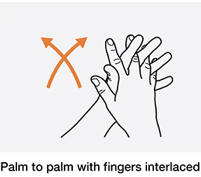
\includegraphics{images/dbs/1.png}
    \caption{}
    \end{figure}
  \end{itemize}
\item
  Prepare collection area. It should look like this:
\end{itemize}

\begin{figure}
\centering
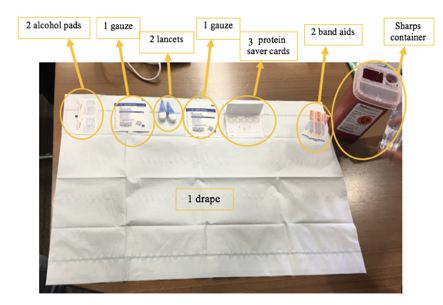
\includegraphics{images/dbs/2.png}
\caption{}
\end{figure}

\hypertarget{vr-headset-setup}{%
\subsubsection{VR Headset Setup}\label{vr-headset-setup}}

\begin{itemize}
\tightlist
\item
  Put VR goggles on for participant.
\item
  Ensure the headset has been charged before it needs to be used.
\item
  Bring the headset and the remote to the DBS Collection room.
\item
  Ask the subject if they are familiar with VR headsets, if they make them feel motion sick, and if they want to use the headset during the DBS protocol.
\item
  One of the RA's should pre-load the BABLab Youtube page:

  \begin{itemize}
  \tightlist
  \item
    Power on the headset (top center button on headset)
  \item
    Go to Library
  \item
    Select Youtube VR
  \item
    Go to the ``Account'' tab
  \item
    Go to the ``Liked Videos'' tab
  \end{itemize}
\item
  Show the child how the controller works:

  \begin{itemize}
  \item
    moving your hand acts as the pointer/cursor
  \item
    to make selections, use the large bumper button on the back or press down the touchpad at the top of the controller

    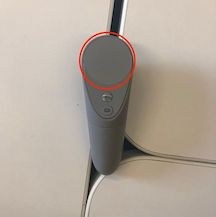
\includegraphics{images/dbs/3.jpeg} ~~~~~~~~~~~~~~~~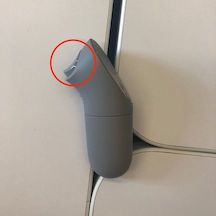
\includegraphics{images/dbs/4.jpeg} ~~~~~~~~~~~~~~~~~~~~~~~~~~~~~~~~~~~~~~
    \emph{Touchpad} ~~~~~~~~~~~~~~~~~~~~~~~~~~~~~~~~~~~~~~~~~~~~~~ \emph{Back bumper}
  \item
    to scroll, move your finger up and down on the touch pad
  \item
    to go back to the movie selection list, press the upper round button below the touchpad

    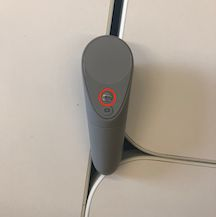
\includegraphics{images/dbs/5.jpeg}
    ~~~~~~~~~~~~~~~~~~~~~~~~~~~~~~~~~~~~~~~~~~~~~~~~~~~~~~~~~~~~~~~~~~~~~~~~~~~~~~~~~~~~~~~~~~~~~~~~ \emph{Back button}
  \end{itemize}
\item
  To put on the headset, loosen the side velcro straps and ask the child to hold the goggles in a comfortable position on their face. If the child wears glasses, they should be fine to use the headset while wearing them.
\item
  Tighten the straps so that the headset stays on its own but isn't uncomfortable for the child to wear.
\item
  Tell them they can watch any of the videos on the playlist.
\item
  Periodically check in with the child to ensure they aren't feeling motion sick or uncomfortable in any way.
\item
  After the DBS is completed, take the headset off the child and power it down.
\end{itemize}

\hypertarget{blood-sample-administration}{%
\subsubsection{Blood Sample Administration}\label{blood-sample-administration}}

\begin{itemize}
\tightlist
\item
  Place heating pad on participant's hand, making sure to cover fingers. Set to low or medium heat.

  \begin{itemize}
  \tightlist
  \item
    Check to make sure it does not get too hot.
  \item
    Set timer for 10 minutes.
  \end{itemize}
\item
  When 10 minutes are up, put on gloves. Have participant pull up heating pad and hold it with their free hand on the upper arm. Make sure the heating pad cable is not in the way of collection.
\item
  Clean middle or ring finger with alcohol and wipe with gauze.
\item
  Prick finger pad slightly off-center toward the side closest to the pinky finger and immediately dispose of lancet in sharps container.
\item
  Wipe first drop with gauze then start collecting on Whatman Protein cards in numbered order.
\item
  When finished, wipe with gauze, put pressure to stop bleeding and apply bandage.
\item
  Remove gloves, use hand sanitizer immediately, then wash hands ASAP.
\end{itemize}

\hypertarget{precautions}{%
\subsubsection{Precautions}\label{precautions}}

\begin{itemize}
\tightlist
\item
  Before, during and after the procedure, ask if the participant is feeling lightheaded.
\item
  Check the participant's complexion - turning pale is a warning sign for impeding faintness.
\item
  If participant feels faint/lightheaded, terminate the procedure, ask them to bend forward, and place their head between their knees. You may apply a cold compression to the back of the neck to speed up recovery.
\item
  Stay with them for at least 15 minutes until they feel completely fine.
\item
  Report the incident to Bridget.
\end{itemize}

\hypertarget{sop-for-fainting-emergency}{%
\subsubsection{SOP for Fainting Emergency}\label{sop-for-fainting-emergency}}

\begin{itemize}
\tightlist
\item
  In case of fainting or any warning symptoms, lay the participant down flat on a surface on their back and elevate their feet if possible (to a level higher than their heart, about 30cm).
\item
  Loosen any constrictive clothing/belts etc.
\item
  Symptoms usually disappear after a short rest.
\item
  If the participant does not regain consciousness within 1 minute, call 911.
\item
  If the participant regains consciousness, avoid having him/her get up too quickly.
\item
  Have them sit for at least 15 minutes until they feel completely fine.
\item
  Offer water or warm sweet drinks.
\item
  Report the incident to Bridget.
\end{itemize}

\hypertarget{sop-for-biohazard-spill-emergency}{%
\subsubsection{SOP for Biohazard Spill Emergency}\label{sop-for-biohazard-spill-emergency}}

\begin{itemize}
\tightlist
\item
  Equipments:

  \begin{itemize}
  \tightlist
  \item
    Disinfectant (Sodium Hypochlorite (Bleach))
  \item
    Absorbent materials sufficient to completely cover spilled liquid and can be disposed (e.g.~paper towels)
  \item
    Physical tools that allow safe handling of sharp materials (e.g.~tongs, forceps, broom/dustpan)
  \item
    Warning signs to notify others that a spill occurred in the area
  \end{itemize}
\item
  Check self for contamination and change PPE if necessary.
\item
  Put on new PPE to proceed with clean up.
\item
  Pick up broken glass/sharps with available physical tools and dispose as biohazardous sharps.
\item
  Place absorbent materials on and around spill.
\item
  Put disinfectant on paper towels and let it sit for at least 5 minutes.
\item
  Dispose of absorbent materials as biohazardous waste.
\item
  Repeat step 4-6 as necessary.
\item
  Remove PPE and wash hands with soap and water.
\item
  Report all spills to Bridget.
\end{itemize}

\emph{Note: Only proceed with biohazardous spill cleanup if you feel comfortable;
Always use physical tools for handling sharps.}

\hypertarget{sop-for-incident-response-and-reporting}{%
\subsubsection{SOP for Incident Response and Reporting}\label{sop-for-incident-response-and-reporting}}

An exposure incident is specific contact with hazardous agents. Exposure incidents at UCLA must be reported, investigated, and documented by UCLA Insurance \& Risk Management; Environment, Health \& Safety; and/or the supervisor of the facility.

\begin{itemize}
\tightlist
\item
  Notify all personnel in the room of the incident.
\item
  Move exposed individual(s) to a safe location, taking care to not spread biohazardous materials.
\item
  Remove contaminated clothing, turn exposed areas inward, and place in a leak-proof bag or container for future decontamination.
\item
  Wash skin with soap and water for 15 minutes.
\item
  Go directly to the Occupational Health Facility at 67-120 CHS (M-F, 7am-4pm) or the RRMC ER.
\item
  Notify Bridget ASAP.
\item
  Report the incident to EH\&S within 8 hours (24-hour hotline: 310-825-9797).
\item
  Record the incident in the Incident and Near Miss Log in the Biosafety Manual.
\end{itemize}

\emph{Note: Keep an extra set of clothes or shoes available to replace contaminated items.}

\hypertarget{storage-of-protein-cards}{%
\subsection{Storage of Protein Cards}\label{storage-of-protein-cards}}

\begin{itemize}
\tightlist
\item
  Using a new drape, place the protein cards along the long horizontal midline of the drape.
\item
  Lightly fold the drape in half along the midline, covering the protein cards but ensure no contact between the drape and the blood spots (i.e.~ensure complete exposure of the blood spots).
\item
  Leave the protein cards to dry for 8-24 hours.
\item
  After drying, close the protein cards with the flap (make sure each one is labeled with participant ID, date and card number), and place each card in a separate ziplock bag with a silica gel pack.
\item
  Place the bags in the BABLab freezer box in the -80˚C freezer in room C454 (key in BABLab lockbox).
\end{itemize}

\begin{center}\rule{0.5\linewidth}{0.5pt}\end{center}

\hypertarget{child-questionnaires}{%
\subsection{Child Questionnaires}\label{child-questionnaires}}

\begin{itemize}
\tightlist
\item
  Ask the participant how comfortable they are reading and comprehending in English
\item
  If not fully comfortable, read the questionnaires for the participant
\item
  Read the first questionnaire - the SS - to all participants
\end{itemize}

\hypertarget{children-8-under}{%
\subsubsection{Children 8 \& Under}\label{children-8-under}}

\begin{itemize}
\tightlist
\item
  The researcher will need to read all questions to child
\item
  PEDSQL GI \& PEDSQL F need the laminated face sheet
\end{itemize}

\begin{center}\rule{0.5\linewidth}{0.5pt}\end{center}

\hypertarget{parent-protocols}{%
\section{Parent Protocols}\label{parent-protocols}}

\hypertarget{ksads}{%
\subsection{KSADS}\label{ksads}}

\hypertarget{audio-recording}{%
\subsubsection{Audio Recording}\label{audio-recording}}

\begin{itemize}
\tightlist
\item
  Make a separate recording for each KSADS administered if there is more than one child in one session.
\end{itemize}

\textbf{Step-by-step guide on how to use recorder:}

\emph{Step 1: Press and hold highlighted Power button to turn recorder.}

\begin{figure}
\centering
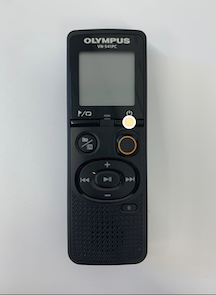
\includegraphics{images/ksads/1.png}
\caption{}
\end{figure}

\emph{Step 2: Press highlighted button until ``TALK'' appears on the screen. Now you are on the ``Talk'' setting.}

\begin{figure}
\centering
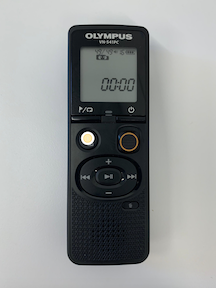
\includegraphics{images/ksads/2.png}
\caption{}
\end{figure}

\emph{Step 3: Push highlighted button up to start recording. Push down to stop recording.}

\begin{figure}
\centering
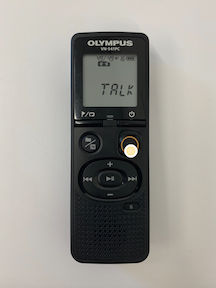
\includegraphics{images/ksads/3.png}
\caption{}
\end{figure}

\hypertarget{using-the-ipad-for-ksads-summary-checklist}{%
\subsubsection{Using the iPad for KSADS Summary Checklist}\label{using-the-ipad-for-ksads-summary-checklist}}

\begin{itemize}
\tightlist
\item
  Before the start of every session, be sure to duplicate and rename all the KSADS documents in Acrobat (25 documents per participant) and rename them (MBBXXX\_KSADS\_suppX\_XXX).

  \begin{itemize}
  \tightlist
  \item
    \emph{Note 1:} This may take a while, especially if there are more than one participant, so be sure to do it ahead of time.
  \item
    \emph{Note 2:} With multiple participants in one session, keep them all on the same iPad as the same iPad will be used to administer all KSADS.
  \end{itemize}
\item
  Follow instructions below on how to duplicate and rename the documents:

  \begin{itemize}
  \item
    Turn on iPad and go to the ``Acrobat'' app.
  \item
    Your screen should look like this. If it does not, tap on ``Files'' at the bottom, and ensure that the Locations is set to ``On This iPad''.

    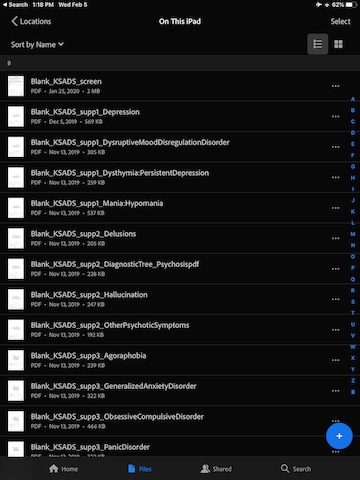
\includegraphics{images/ksads/4.png}
  \item
    For each document, tap the three horizontal dot to the right, and select ``Duplicate''.
    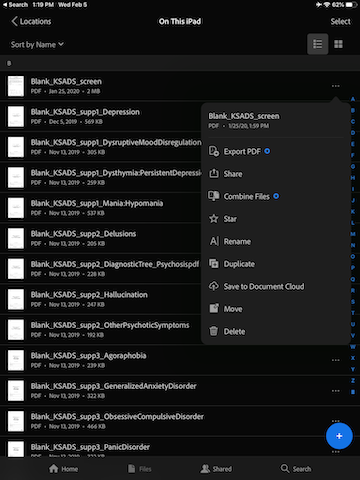
\includegraphics{images/ksads/5.png}
  \item
    The duplicated document should appear right below the original document.
  \item
    Tape the three horizontal dot to the right of the duplicated document, and select ``Rename''.
    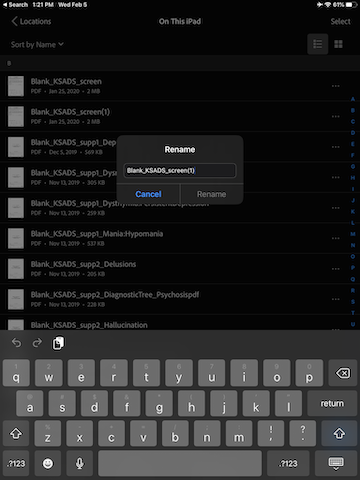
\includegraphics{images/ksads/6.png}
  \item
    Replace the word ``Blank'' with the participant ID, and remove the ``(1) at the end of the name. For example, if the participant ID is MBB001, the name of the duplicated document should be: MBB001\_KSADS\_screen
  \item
    Do the same for all 25 documents (Duplicate, Rename).
  \end{itemize}
\end{itemize}

\begin{center}\rule{0.5\linewidth}{0.5pt}\end{center}

\hypertarget{home-kit}{%
\subsection{Home Kit}\label{home-kit}}

Please refer to the diagram below for the complete list of items in a home kit:

\begin{figure}
\centering
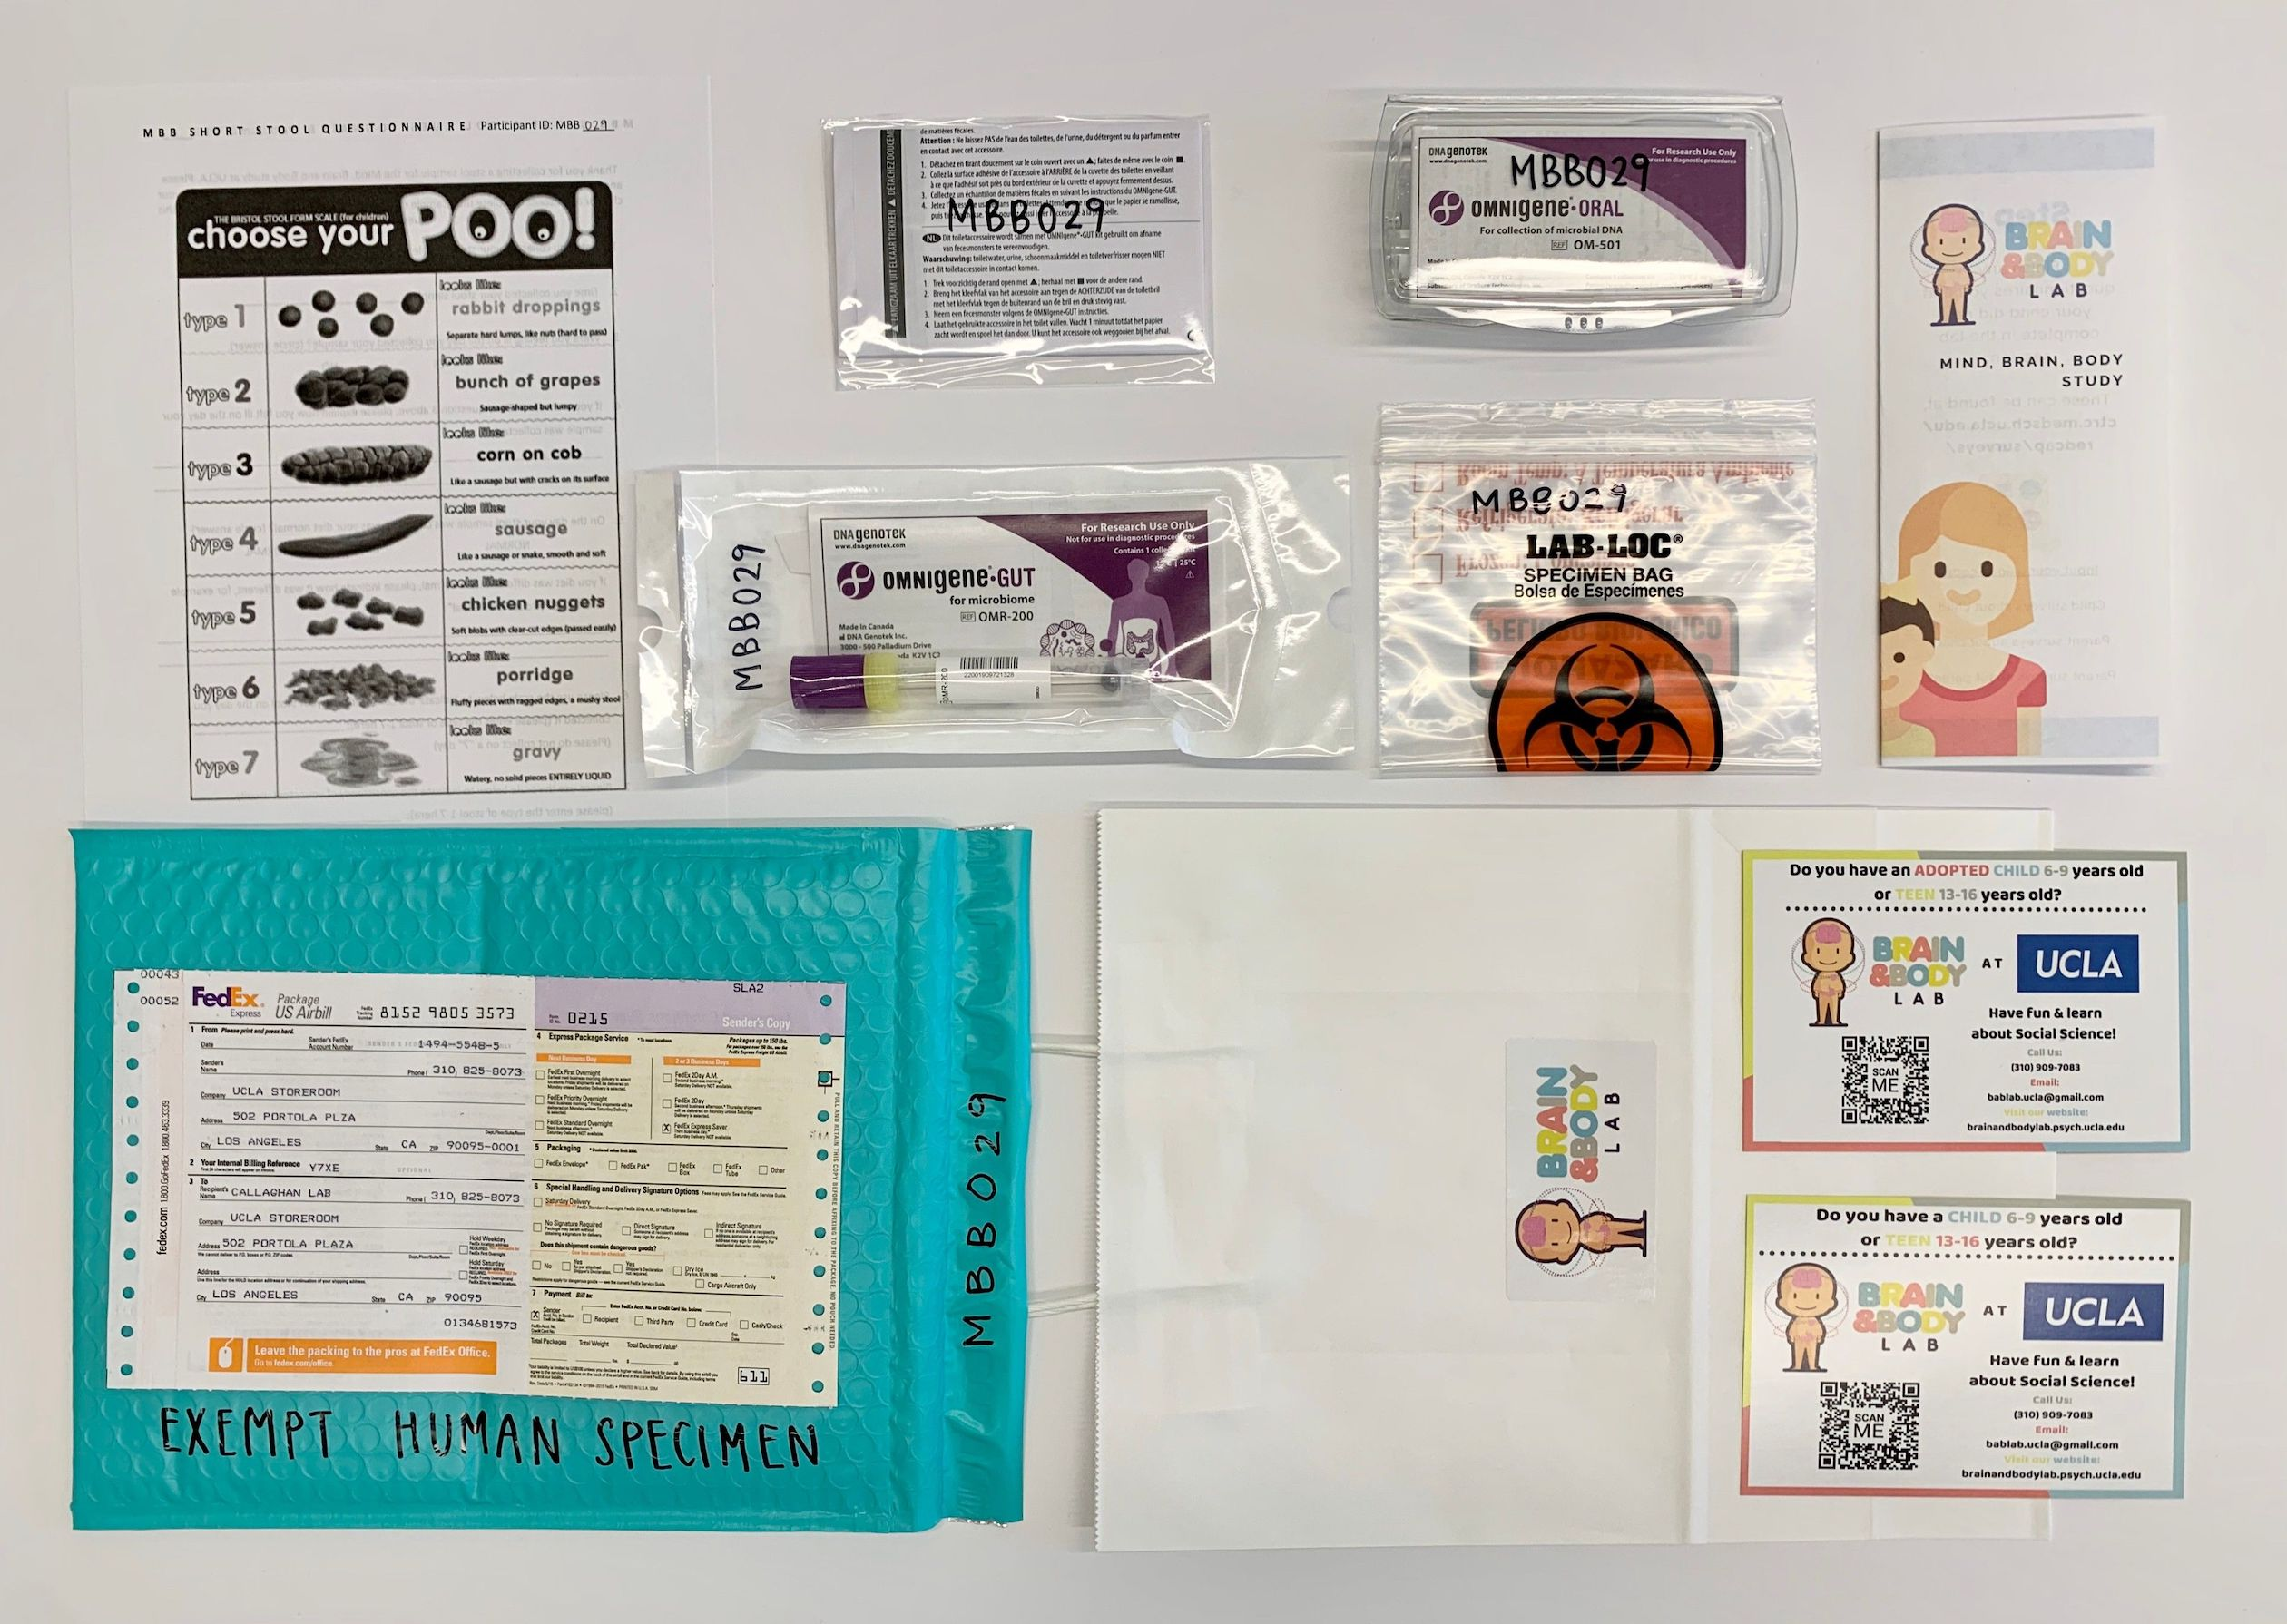
\includegraphics{images/home_kit/1.jpeg}
\caption{}
\end{figure}

\begin{itemize}
\tightlist
\item
  Take a white paper gift bag and paste a BABLab sticker at the center of the bag (one side only).
\item
  Take a blue mailer and paste a FedEx slip on the front. Label the mailer with ``Exempt Human Specimen'' and the participant ID.
\item
  Label the following 4 items with the participant ID and put them in the blue mailer:

  \begin{itemize}
  \tightlist
  \item
    a gut kit
  \item
    a toilet hat
  \item
    an oral kit
  \item
    a biohazard bag
  \end{itemize}
\item
  Put two MBB note cards (one biological and one adoption) in the gift bag.
\item
  Print and insert the Bristol Stool Scale.
\item
  Print, fill-out and insert MBB brochure.
\end{itemize}

\begin{center}\rule{0.5\linewidth}{0.5pt}\end{center}

\hypertarget{participant-payment}{%
\subsection{Participant Payment}\label{participant-payment}}

\textbf{Participant Reimbursement Signature}

\hypertarget{setting-up-the-ipad}{%
\subsubsection{Setting up the iPad}\label{setting-up-the-ipad}}

\begin{itemize}
\item
  To obtain participant's signature for payment receipt form, log into the BABLab iPad 1 or 2 with the password ``0719''.
\item
  Make sure the Apple Pencil is paired with the iPad by going into ``Settings'' and then selecting ``Bluetooth'', ensuring that ``Apple Pencil'' is connected.

  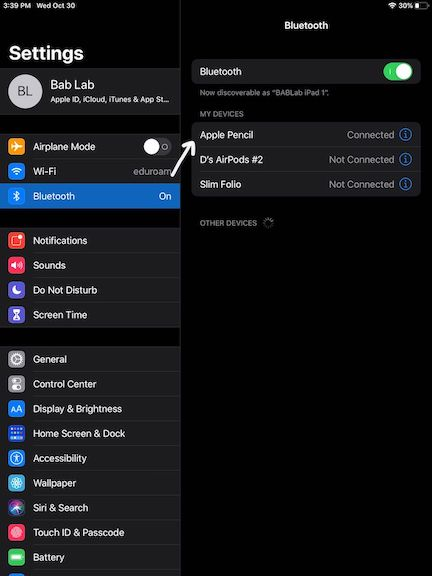
\includegraphics{images/payment/1.jpeg}
\item
  If the Apple Pencil is not connected, remove the cap of the pencil and insert it into the charging port of the iPad. A pop-up should appear to ask you to ``pair'' the devices.

  \begin{figure}
  \centering
  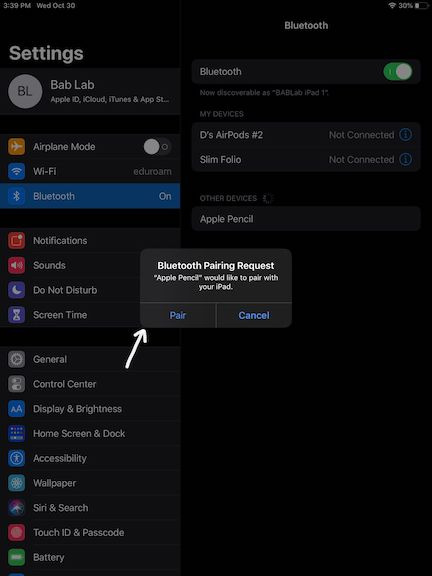
\includegraphics{images/payment/2.jpeg}
  \caption{}
  \end{figure}
\end{itemize}

\hypertarget{to-obtain-signature}{%
\subsubsection{To Obtain Signature}\label{to-obtain-signature}}

\begin{itemize}
\item
  Click the ``Acrobat'' app on the iPad.

  \begin{figure}
  \centering
  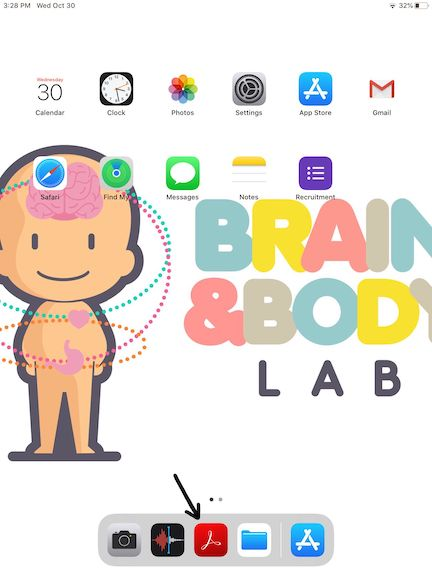
\includegraphics{images/payment/3.jpeg}
  \caption{}
  \end{figure}
\item
  Select the file ``Payment Receipt Signature Form BABLab''.

  \begin{figure}
  \centering
  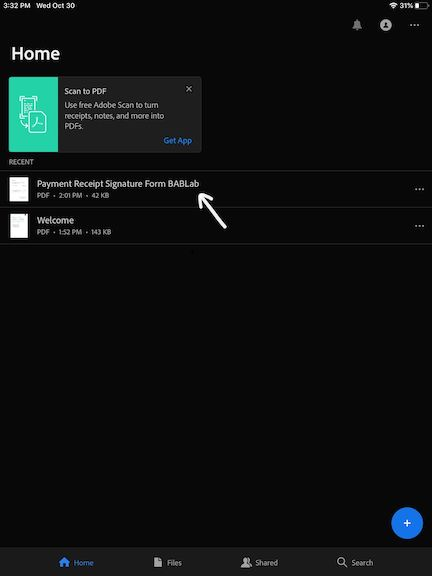
\includegraphics{images/payment/4.jpeg}
  \caption{}
  \end{figure}
\item
  Double tap the screen with the pencil. Ensure the pen icon is selected and fill in the payment receipt number. Now the form is ready to be filled out by the participant.

  \begin{figure}
  \centering
  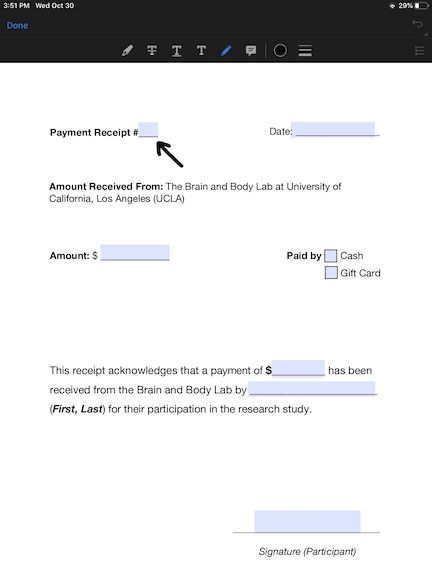
\includegraphics{images/payment/5.jpeg}
  \caption{}
  \end{figure}
\item
  Ask the participant to fill out every highlighted spaces (except for the payment receipt \#).
\item
  After every space has been completed, click ``Done'' on the top left corner.

  \begin{figure}
  \centering
  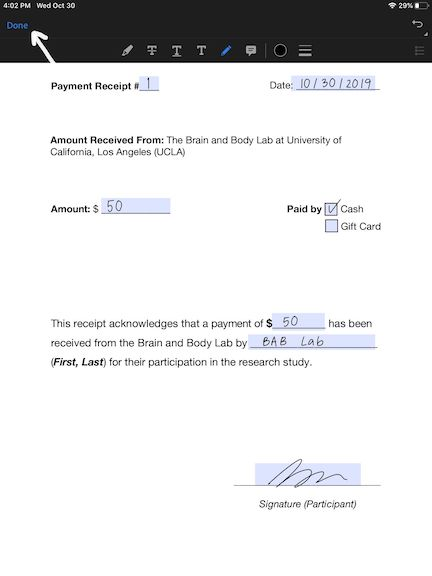
\includegraphics{images/payment/6.jpeg}
  \caption{}
  \end{figure}
\end{itemize}

\hypertarget{to-save-the-filled-out-form}{%
\subsubsection{To Save the Filled-Out Form}\label{to-save-the-filled-out-form}}

\begin{itemize}
\item
  Click the ``share'' icon.

  \begin{figure}
  \centering
  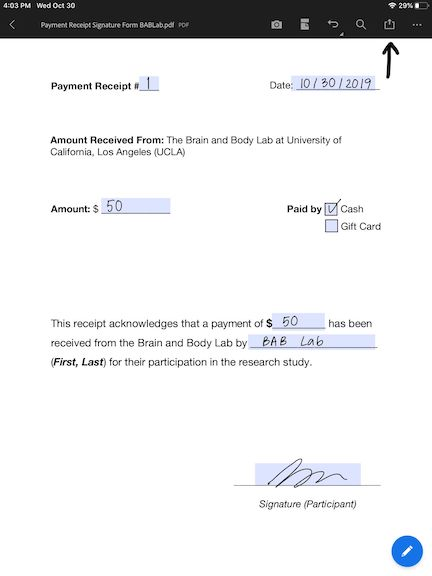
\includegraphics{images/payment/7.jpeg}
  \caption{}
  \end{figure}
\item
  Click ``Share a Copy'' at the bottom.

  \begin{figure}
  \centering
  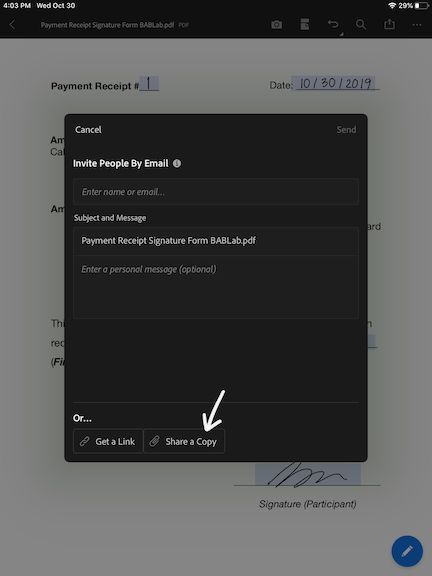
\includegraphics{images/payment/8.jpeg}
  \caption{}
  \end{figure}
\item
  Click ``AirDrop'' to send the file to ``Brain's MacBook Air''.

  \begin{figure}
  \centering
  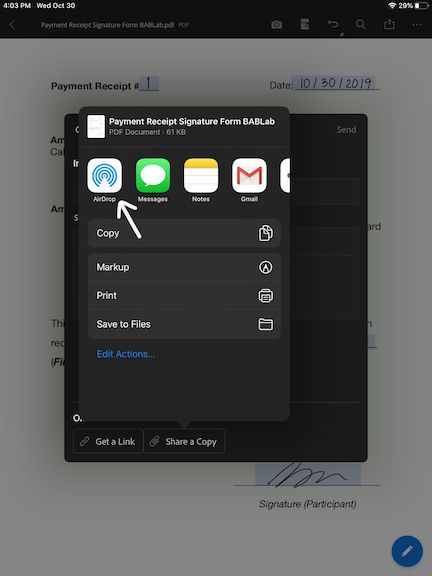
\includegraphics{images/payment/9.jpeg}
  \caption{}
  \end{figure}
\item
  Save the file to a folder named ``Reimbursement\_signed'' on the MacBook Air.
\item
  Return to the iPad and tap the screen once. A box should appear that selects all the participant's input. Clear the input by clicking on the trash icon on the top right.

  \begin{figure}
  \centering
  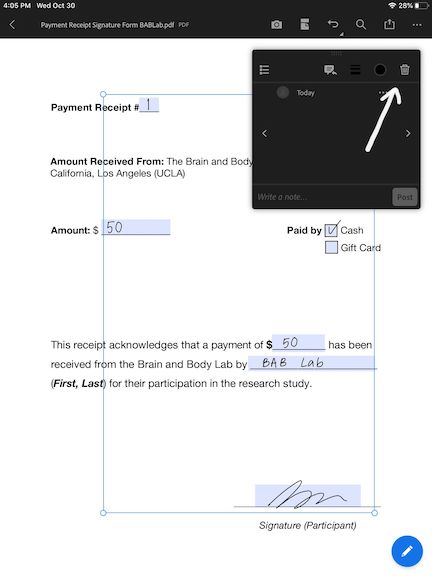
\includegraphics{images/payment/10.jpeg}
  \caption{}
  \end{figure}
\item
  Now the file in Acrobat on the iPad is ready to be used for the next participant.
\end{itemize}

\hypertarget{post-lab-protocols}{%
\section{Post-Lab Protocols}\label{post-lab-protocols}}

\hypertarget{stool-sample}{%
\subsection{Stool Sample}\label{stool-sample}}

\hypertarget{sample-quality}{%
\subsubsection{Sample Quality}\label{sample-quality}}

\begin{itemize}
\tightlist
\item
  Put on gloves.
\item
  Open the mailer to ensure that it contains both the stool sample (in biohazard bag) and the Bristol Stool Scale.
\item
  Check for quality of the stool sample by shaking it up and down vigorously (keep the sample in the biohazard bag), then check for its consistency and color - It should be a dark-brown liquid.
\item
  If stool sample does not meet requirement (e.g.~sample is in solid form or amount collected is too little), contact the family to see if they would be willing to send another sample with compensation.
\item
  Contact family if the Bristol Stool Scale is missing in the mailer.
\end{itemize}

\hypertarget{sample-transfer}{%
\subsubsection{Sample Transfer}\label{sample-transfer}}

\begin{itemize}
\tightlist
\item
  Wear appropriate PPE:

  \begin{itemize}
  \tightlist
  \item
    Gloves
  \item
    Lab coat
  \item
    Safety glasses
  \item
    Surgical Mask
  \item
    Closed-toe shoes
  \item
    Long pants
  \item
    Hair tied back
  \end{itemize}
\item
  Prepare your station and ensure that you have the following:

  \begin{itemize}
  \tightlist
  \item
    Drape
  \item
    2.0mL cryogenic vials
  \item
    Stool samples in biohazard bag
  \item
    Test tube racks
  \item
    Transport box with divider
  \item
    Sharpie for labeling
  \end{itemize}
\end{itemize}

\textbf{Steps:}

\begin{itemize}
\tightlist
\item
  Lay a new drape on the work station and keep all equipments and sample on the drape throughout the transfer process.
\item
  With the stool sample collection vial still in the biohazard bag, shake it up and down vigorously.
\item
  Take the stool sample out of the bag and put it on the test tube rack.
\item
  Untwist two 2.0mL vials and place them on the test tube rack.
\item
  Untwist the stool sample collection vial, and carefully pour the sample into the first 2.0mL vial. (It's okay if the ball does or does not get transferred)
\item
  Stop pouring when solution reached the 1.8mL line to prevent overflow, and pour the remaining sample (if any) in a second 2.0mL vial.
\item
  Cap the 2.0mL vials tightly to prevent spills.
\item
  Label the 2.0mL vials with a sharpie, ensure it has the participant ID and vial number.
\item
  Place the labeled 2.0mL vials in the transport box with divider.
\item
  Close the now-empty stool sample collection vial, put it back in the biohazard bag, and dispose it in the biohazard waste bin.
\item
  Clean up work station, dispose the drape, and wipe down the table top with disinfectant wipe.
\item
  Remove PPE and wash hands with soap and water thoroughly.
\item
  Bring the transport box to C454 where the -80˚C freezer is located (key in BABLab Lock Box).
\item
  Place the 2.0mL vials in their designated space in the freezer box (in accordance to the Sample Storage Log Diagram).
\item
  Log the sample in the \href{https://app.box.com/file/630322897864}{Sample Storage Log}.
\end{itemize}

\begin{center}\rule{0.5\linewidth}{0.5pt}\end{center}

\hypertarget{data-review-audit}{%
\subsection{Data Review \& Audit}\label{data-review-audit}}

\hypertarget{follow-up-completed-by-scheduling-coordinator}{%
\subsubsection{Follow-Up (completed by Scheduling Coordinator)}\label{follow-up-completed-by-scheduling-coordinator}}

\begin{itemize}
\tightlist
\item
  Before sending Home Reminder 3, make sure RA's have completed Data Entry, Data Quality Check 1, and Data Quality Check 2.
\item
  After sending Home Reminder 3 - create blank Trello card for participant on \emph{In Data Review} list.
\end{itemize}

\hypertarget{data-review-completed-by-lab-manager-1}{%
\subsubsection{Data Review (completed by Lab Manager \#1)}\label{data-review-completed-by-lab-manager-1}}

\begin{itemize}
\tightlist
\item
  Once card has been created, do Data Review.
\item
  After completing Data Review, move card to \emph{Good Sample}, \emph{Bad Sample}, or \emph{No Sample} list based on the stool sample.
\end{itemize}

\hypertarget{data-audit-completed-by-lab-manager-2}{%
\subsubsection{Data Audit (completed by Lab Manager \#2)}\label{data-audit-completed-by-lab-manager-2}}

\textbf{If Good Sample:}

\begin{itemize}
\tightlist
\item
  Send payment, thank you letter, and certificate via mail.
\item
  Send {[}MBB - PAID{]} email and attach thank you letter, certificate, and parent report (including outstanding items).
\item
  Move to \emph{Paid} list.
\item
  One week after payment is sent, check outstanding items do Audit Call \#1.
\item
  One week following Audit Call \#1, check outstanding items do Audit Call \#2.
\item
  Within 2 days, check outstanding items and do Audit Call \#3.
\item
  After Audit Call \#3 (or all items completed), send {[}MBB - DONE{]} email and move to \emph{Done} list.
\end{itemize}

\textbf{If Bad Sample:}

\begin{itemize}
\tightlist
\item
  Send payment, thank you letter, and certificate via mail. Include a new stool sample kit.
\item
  Send {[}MBB - PAID{]} email and attach thank you letter, certificate, and parent report (including outstanding items - emphasize stool sample kit).
\item
  Move to \emph{Paid} list in Trello.
\item
  One week after payment is sent, check outstanding items do Audit Call \#1.
\item
  One week following Audit Call \#1, check outstanding items do Audit Call \#2.
\item
  Within 2 days, check outstanding items and do Audit Call \#3.
\item
  After Audit Call \#3 (or all items completed), send {[}MBB - DONE{]} email and move to \emph{Done} list.
\end{itemize}

\textbf{If No Sample:}

\begin{itemize}
\tightlist
\item
  Send {[}MBB - UNPAID{]} email and attach thank you letter, certificate, and parent report (including outstanding items - emphasize stool sample kit).
\item
  Leave participant on Unpaid list.
\item
  If stool sample recieved - send payment, thank you letter, and certificate via mail and move to \emph{Paid} list.
\item
  If stool sample not received, one week after email is sent, check outstanding items do Audit Call \#1.
\item
  One week following Audit Call \#1, check outstanding items do Audit Call \#2.
\item
  Within 2 days of Audit Call \#2, check outstanding items and do Audit Call \#3.
\item
  After Audit Call \#3 (or all items completed), send {[}MBB - DONE{]} email and move to \emph{Done} list.
\end{itemize}

\hypertarget{wave-1-online}{%
\chapter{Wave 1 Online}\label{wave-1-online}}

\hypertarget{checklists-online}{%
\section{Checklists Online}\label{checklists-online}}

\begin{center}\rule{0.5\linewidth}{0.5pt}\end{center}

\hypertarget{initial-online-checklist}{%
\subsection{Initial Online Checklist}\label{initial-online-checklist}}

\textbf{Scheduling and Confirmation}

\begin{itemize}
\tightlist
\item
  Schedule lab session 2 weeks in advance from ``package mailing day'' (see package preparation in pre-session checklist)
\item
  Make Zoom link with scheduled session time and save to google calendar
\item
  Send confirmation email (in templates)

  \begin{itemize}
  \tightlist
  \item
    Attach \href{https://ucla.app.box.com/file/665452959932}{Next Steps}, \href{https://ucla.app.box.com/file/680632734387}{Computer Zoom Download Instructions}, and \href{https://ucla.app.box.com/file/680631353662}{Phone Zoom Download Instructions}
  \end{itemize}
\end{itemize}

\textbf{Enrollment}

\begin{itemize}
\tightlist
\item
  Create participant Box folder using MBB\_template (delete blank README from newly created folder)
\item
  Enroll participant in Wave 1 on REDCap
\item
  Fill participant instrument on REDCap
\item
  Fill counterbalance order on REDCap (Checklist - Lab Session Child Instrument)
\end{itemize}

\textbf{Calendar}

\begin{itemize}
\tightlist
\item
  Create MBB calendar event lab session and invite researcher
\item
  Create MBB calendar event to mail study package to participant
\item
  Create MBB calendar event lab session reminder 1 (email) (1 week prior)
\item
  Create MBB calendar event lab session reminder 2 (email and call) (3 days prior)
\item
  Create MBB calendar event to send home session reminder 1 (email) (on the day that home session is scheduled)
\item
  Create MBB calendar event to make home session reminder 1 (call) (2 days after scheduled home session)
\item
  Create MBB calendar event to send home session reminder 2 (email) (4 days after scheduled home session)
\item
  Create MBB calendar event to send home session reminder 3 (email) (6 days after scheduled home session)
\end{itemize}

\textbf{Reminders}

\begin{itemize}
\tightlist
\item
  Send lab session reminder 1 email (in templates - attach next steps, consent/assent, zoom instructions, confirm if package is received)
\item
  Send lab session reminder 2 email (in templates - attach previous, confirm if package is received)
\item
  Confirm package is delivered and received
\item
  Confirm participant

  \begin{itemize}
  \tightlist
  \item
    Preferably by phone
  \item
    Update lab session calendar status
  \end{itemize}
\end{itemize}

\begin{center}\rule{0.5\linewidth}{0.5pt}\end{center}

\hypertarget{pre-online-session-checklist}{%
\subsection{Pre-Online Session Checklist}\label{pre-online-session-checklist}}

\hypertarget{package-preparation}{%
\subsubsection{Package preparation}\label{package-preparation}}

\emph{(prepare and send from all scheduled participants in the last week, to be mailed 2 weeks prior to session)}

\begin{itemize}
\tightlist
\item
  Print {[}What is in this package?{]}
\item
  Print \href{https://ucla.app.box.com/file/668504120930}{Reward Board} (plus gold star stickers)
\item
  Print/Staple Parent Questionnaire Booklet (in this order)

  \begin{enumerate}
  \def\labelenumi{\arabic{enumi}.}
  \tightlist
  \item
    Parent Questionnaire Cover Page/Parent Proxy Intro
  \item
    pedsql\_gi\_parentproxy
  \item
    pedsql\_wb\_parentproxy
  \item
    peds1l\_f\_parentproxy
  \item
    easy\_revised
  \item
    cshq\_revised
  \item
    mb\_metadat
  \item
    med\_check
  \item
    pds
  \item
    dhws
  \item
    hpq
  \item
    cssi (for children under 8)
  \item
    fci
  \item
    iai
  \item
    Demographics
  \item
    financial
  \item
    Parent Self Intro
  \item
    bdi
  \item
    parent\_stress
  \item
    COVID\_objective
  \end{enumerate}
\item
  Print/Staple Child Questionnaire Booklet (in this order)

  \begin{enumerate}
  \def\labelenumi{\arabic{enumi}.}
  \tightlist
  \item
    Child Questionnaire Cover Page
  \item
    ss
  \item
    cpic
  \item
    alexithymia
  \item
    cssi (for children over 8)
  \item
    bce\_revised
  \end{enumerate}
\item
  Print/Staple Online Session Booklet (in this order)

  \begin{enumerate}
  \def\labelenumi{\arabic{enumi}.}
  \tightlist
  \item
    Online Session Cover page
  \item
    Fill in codes on \href{https://ucla.app.box.com/file/665449085502}{Participant Info Brochure}
  \item
    \href{https://ucla.app.box.com/file/630327764749}{Pleasant/Unpleasant Events Checklist}
  \item
    Anthropomorphic measurement sheets
  \item
    Saliva Sample Instructions Sheet
  \item
    \href{https://ucla.app.box.com/file/685938821891}{Hair Sample Instructions Sheet}
  \end{enumerate}
\item
  Print/Staple Home Session Booklet (in this order)

  \begin{enumerate}
  \def\labelenumi{\arabic{enumi}.}
  \tightlist
  \item
    Home Session Cover Page
  \item
    \href{https://ucla.app.box.com/file/639652767665}{Contact List} and label with participant ID
  \item
    Stool Sample Instructions Sheet
  \item
    \href{https://app.box.com/file/630326499609}{Bristol Stool Scale} and label with participant ID (MBB Specific Version)
  \end{enumerate}
\item
  Prepare 2 sharpened pencils
\item
  Prepare paper measuring tape (for waist and height measurements)
\item
  Label 2 biohazard bags (with 2 cotton balls in each bag)
\item
  Label 1 cardboard box (for samples)
\item
  Label hair sample kit (aluminum foil 7``x7'', painter's tape with ``root end'' labeled, 1 ziplock bag pre-labeled with participant ID)
\item
  Label stool sample collection kit (collection tube, toilet hat)
\item
  Label saliva sample collection kit (collection tube)
\item
  Insert MBB info cards
\item
  Attach FedEx slip to return mailer
\item
  Label return mailer with ``exempt human specimen'' (in sharpie)
\item
  Take picture of prepaid blue return mailer (marked with MBB number) and file in participant data folder on Box
\item
  Insert all labeled items and forms into blue return mailer
\item
  Insert blue return mailer into study package
\item
  Tape package closed and put BABLAB sticker on (if enough supplies)
\item
  Take a picture of study package with tracking information to file on Box
\item
  Mail package to participant
\end{itemize}

\begin{center}\rule{0.5\linewidth}{0.5pt}\end{center}

\hypertarget{online-session-setup---1-hour-prior}{%
\subsubsection{Online Session Setup - 1 Hour Prior}\label{online-session-setup---1-hour-prior}}

\begin{itemize}
\tightlist
\item
  Prepare session scripts/protocol
\item
  Prepare session checklist with counterbalance order
\item
  Have the Participant's MBB and secondary MBB number on hand
\item
  Preload the following tabs on researcher's computer:

  \begin{itemize}
  \tightlist
  \item
    Consent/Assent picture slideshow
  \item
    Hair Sample Collection video
  \item
    REDCap with child questionnaire codes ready
  \end{itemize}
\item
  Prepare biological sample kits for demonstration during session

  \begin{itemize}
  \tightlist
  \item
    hair sample, saliva sample, stool sample
  \end{itemize}
\item
  Ensure researcher's Zoom security settings are set for study session
\end{itemize}

\begin{center}\rule{0.5\linewidth}{0.5pt}\end{center}

\hypertarget{online-session-checklist}{%
\subsection{Online Session Checklist}\label{online-session-checklist}}

\begin{itemize}
\tightlist
\item
  Session walk-through/package explanation
\item
  Consent/Assent
\item
  Parent-child observation (note recording via Zoom or pre-recording)
\item
  If pre-recorded, instruct participant how to upload to Box
\item
  Explain Questionnaires Parent Proxy or Parent self on second device if available (for parent to complete during Halloween training, Halloween test, and Child Questionnaires)
\item
  Halloween training
\item
  Height
\item
  Weight
\item
  Waist circumference
\item
  Halloween test
\item
  Saliva sample
\item
  Hair sample
\item
  Child Questionnaires
\item
  Stool Sample explanation
\item
  Contact list explanation
\item
  Confirm mailing address for payment
\item
  Schedule time to complete post-session tasks \textasciitilde{}1 week post-session
\item
  Qualitative parent and child free responses (optional)
\end{itemize}

\begin{center}\rule{0.5\linewidth}{0.5pt}\end{center}

\hypertarget{post-online-session-checklist}{%
\subsection{Post-Online Session Checklist}\label{post-online-session-checklist}}

\hypertarget{notes}{%
\subsubsection{Notes}\label{notes}}

\begin{itemize}
\tightlist
\item
  Make note of issues to discuss (if needed) in Boxnote for next core meeting
\end{itemize}

\hypertarget{filing}{%
\subsubsection{Filing}\label{filing}}

\begin{itemize}
\tightlist
\item
  ``Scan'' online session checklist and file in participant folder
\item
  Transfer and rename Zoom recording to Box
\end{itemize}

\begin{center}\rule{0.5\linewidth}{0.5pt}\end{center}

\hypertarget{final-online-checklist}{%
\subsection{Final Online Checklist}\label{final-online-checklist}}

\hypertarget{filing-1}{%
\subsubsection{Filing}\label{filing-1}}

\begin{itemize}
\tightlist
\item
  Make low-res parent child interaction video and save on BABLab External Hard Drive
\item
  Burn all audio and video (low res) files to CD and label/store CD in binder
\item
  Make manila folder for participants to file all hard copies
\end{itemize}

\hypertarget{data-entry}{%
\subsubsection{Data Entry}\label{data-entry}}

\begin{itemize}
\tightlist
\item
  Enter online session checklist data to REDCap
\item
  Enter height, weight, waist to REDCap
\end{itemize}

\hypertarget{reminders}{%
\subsubsection{Reminders}\label{reminders}}

\begin{itemize}
\tightlist
\item
  Home session reminder 1 email sent
\item
  Reminder 1 phone call made
\item
  Home session reminder 2 email sent
\item
  Home session reminder 3 email sent
\end{itemize}

\hypertarget{home-session}{%
\subsubsection{Home Session}\label{home-session}}

\begin{itemize}
\tightlist
\item
  Halloween test delay completed
\item
  Hair sample received
\item
  Saliva sample received
\item
  Stool sample received
\item
  Bristol Stool Scale data received
\item
  Questionnaires received (if paper versions were sent)
\item
  Consent/Assent forms received (if paper versions were sent)
\item
  Contact information sheet received
\end{itemize}

\emph{After package has been received\ldots{}}

\hypertarget{data-entry-1}{%
\subsubsection{Data Entry}\label{data-entry-1}}

\begin{itemize}
\tightlist
\item
  Enter contact list information into recruitment database
\item
  Enter questionnaires data (if paper versions were sent)
\item
  Scan and upload Bristol Stool Scale to Box
\item
  Enter Bristol Stool Scale data to REDCap
\end{itemize}

\hypertarget{filing-2}{%
\subsubsection{Filing}\label{filing-2}}

\begin{itemize}
\tightlist
\item
  File Consent/Assent forms in filing cabinet (consent manila folder)
\item
  File contact list in filing cabinet (contact list manila folder)
\item
  File Bristol Stool Scale in filing cabinet (participant folder)
\item
  File questionnaires in filing cabinet if paper versions were sent (participant folder)
\end{itemize}

\hypertarget{sample-storage}{%
\subsubsection{Sample Storage}\label{sample-storage}}

\begin{itemize}
\tightlist
\item
  Label and store stool sample (add data quality to REDCap)
\item
  Label and store saliva sample
\item
  Label and store hair sample
\item
  Update sample storage log on Box (once all received)
\item
  Upload all sample photos to Box
\end{itemize}

\hypertarget{data-quality}{%
\subsubsection{Data Quality}\label{data-quality}}

\begin{itemize}
\tightlist
\item
  Data quality check 1
\item
  Data quality check 2
\item
  Data review
\item
  Data audit
\end{itemize}

\hypertarget{retention}{%
\subsubsection{Retention}\label{retention}}

\begin{itemize}
\tightlist
\item
  Prep report card
\item
  Send report card email (in templates - attach report card)
\item
  Update participant Wave 2 status
\end{itemize}

\hypertarget{reimbursement}{%
\subsubsection{Reimbursement}\label{reimbursement}}

\begin{itemize}
\tightlist
\item
  Mail payment with science kits
\item
  Take a picture of tracking information and upload to Box
\item
  Log participant payment in reimbursement log book
\item
  Log participant payment in reimbursement spreadsheet
\end{itemize}

\begin{center}\rule{0.5\linewidth}{0.5pt}\end{center}

\hypertarget{pre-online-session-protocols}{%
\section{Pre-Online Session Protocols}\label{pre-online-session-protocols}}

\hypertarget{recruitment-online}{%
\subsection{Recruitment Online}\label{recruitment-online}}

\hypertarget{pre-screening}{%
\subsubsection{Pre-Screening}\label{pre-screening}}

\begin{enumerate}
\def\labelenumi{\arabic{enumi}.}
\tightlist
\item
  Check if participant is in Recruitment Database

  \begin{itemize}
  \tightlist
  \item
    If not, add them to the Recruitment Database
  \end{itemize}
\item
  Check if participant is in ID Drive

  \begin{itemize}
  \tightlist
  \item
    If yes, check if they have a Screener ID
  \item
    If not, assign them a Screener ID once contact has been established based on the next available Screener ID \# in REDCap and proceed with screening
  \item
    If yes, proceed with screening under existing Screener ID in REDCap
  \end{itemize}
\end{enumerate}

\hypertarget{screening}{%
\subsubsection{Screening}\label{screening}}

\begin{enumerate}
\def\labelenumi{\arabic{enumi}.}
\tightlist
\item
  To screen a new participant click ``Add / Edit Records''
  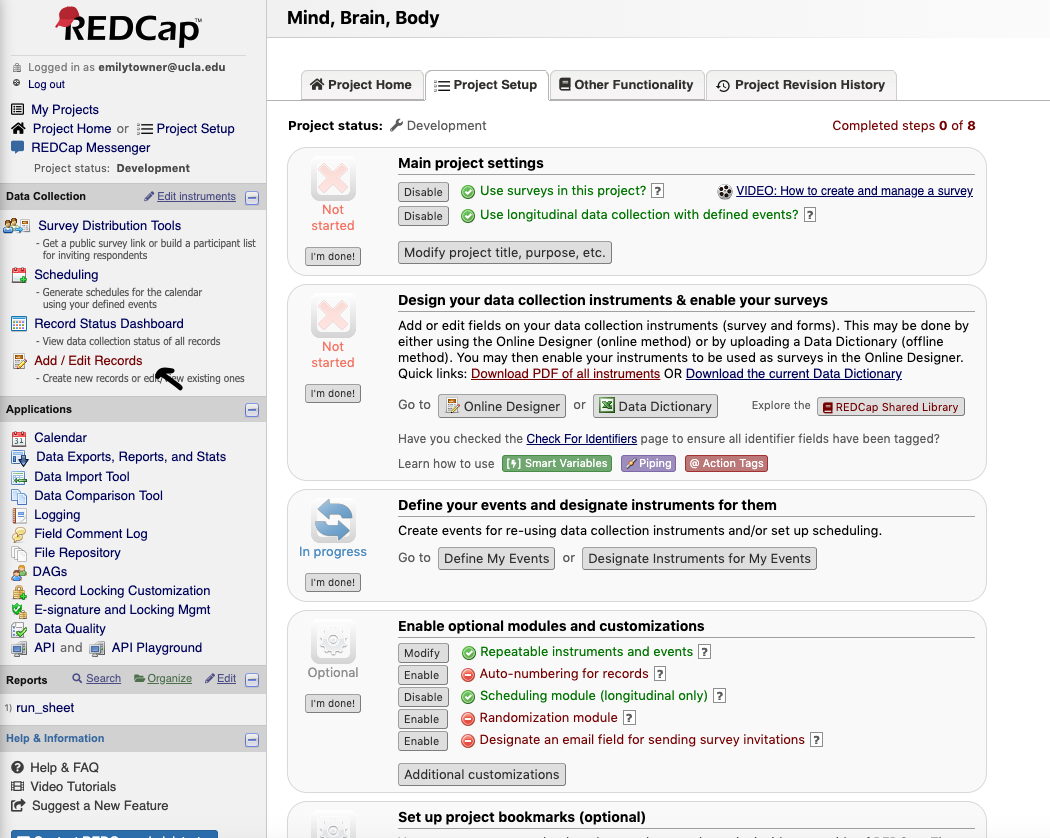
\includegraphics{images/redcap_screening/1.png}
\item
  Click to enter a new Subject ID

  \begin{itemize}
  \tightlist
  \item
    Make sure Arm 1: Recruitment is selected
  \end{itemize}
\item
  Type ``SMBB\#'' (Screener ID) to create a record and hit ``Enter''

  \begin{itemize}
  \tightlist
  \item
    Make sure to link the participants Screener ID and their name on the \textbf{ID Drive ONLY}
  \item
    Before creating a new record, be sure to check the ID Drive to see if the participant already has an existing Screener ID
  \item
    If a record exists, add a new instance of the screen instead of creating a new record
    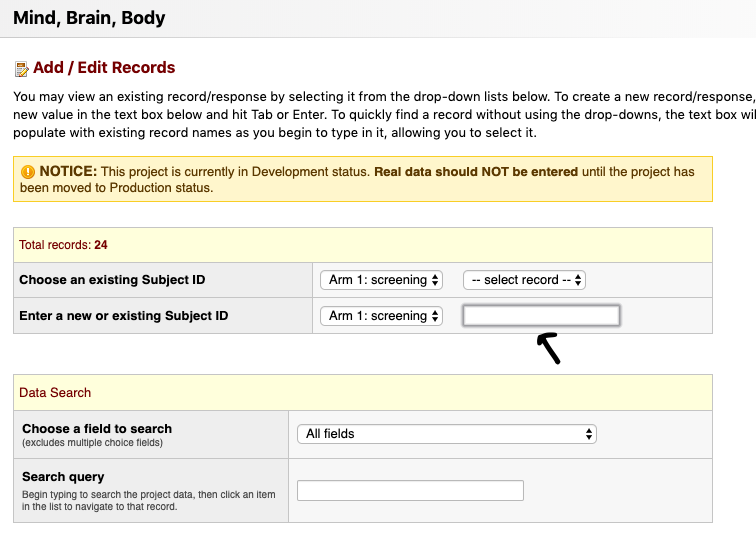
\includegraphics{images/redcap_screening/2.png}
  \end{itemize}
\item
  The screening arm contains two parts

  \begin{itemize}
  \tightlist
  \item
    The screen
  \item
    The wave1\_status

    \begin{itemize}
    \tightlist
    \item
      The wave1\_status is to be updated after the first and each subsequent contact
      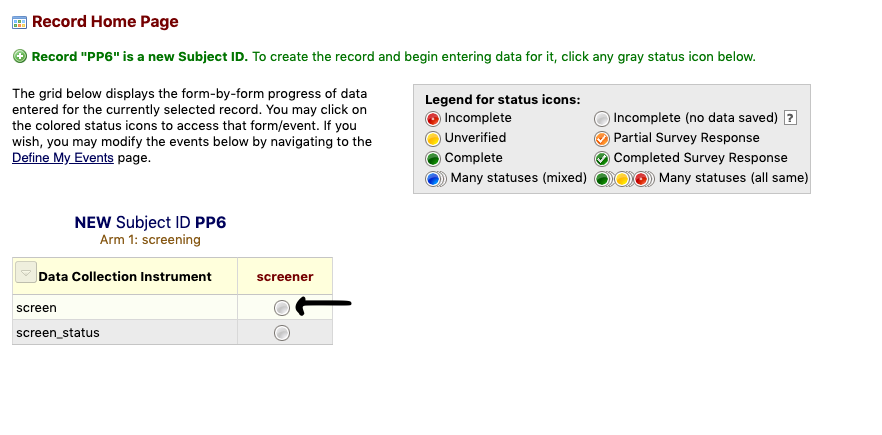
\includegraphics{images/redcap_screening/3.png}
    \end{itemize}
  \end{itemize}
\item
  Click on the radio button in the ``screen'' row to screen the participant
  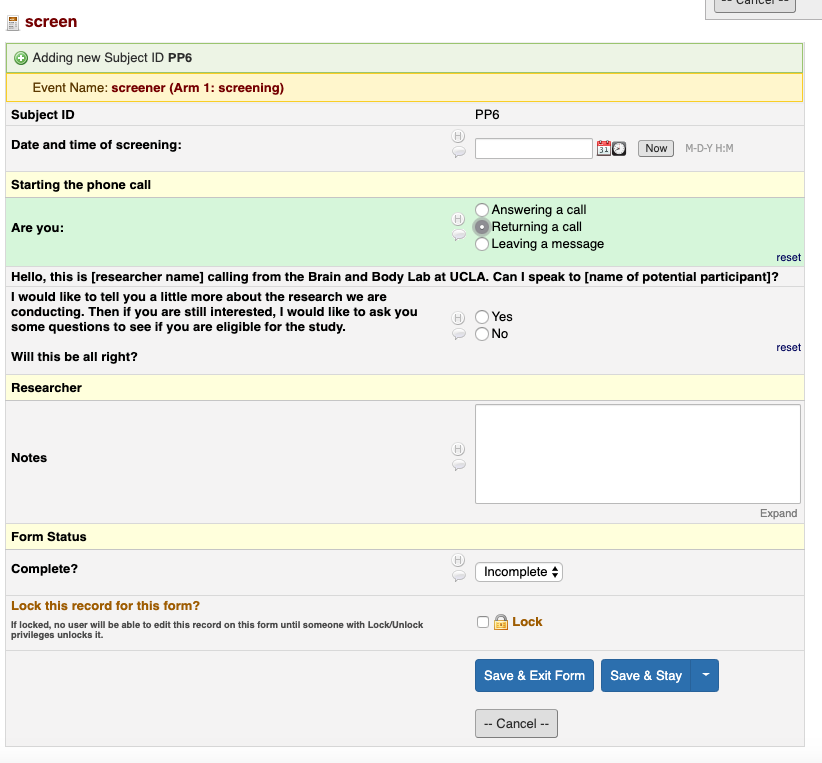
\includegraphics{images/redcap_screening/4.png}
\item
  Click ``Now'' to enter today's date and time
\item
  Select the appropriate choice to start the phone call and follow the skip logic
\item
  Follow the skip logic to the end

  \begin{itemize}
  \tightlist
  \item
    For items without a text field, write the information down in the Recruitment database (This identifying information cannot be on REDCap)
  \end{itemize}
\item
  Once done, select ``Complete'' and ``Save \& Exit Form''

  \begin{itemize}
  \tightlist
  \item
    The screen can be entered multiple times - for instance if there are multiple phone calls or contacts
  \item
    It is important to keep a record of all instances of contact
    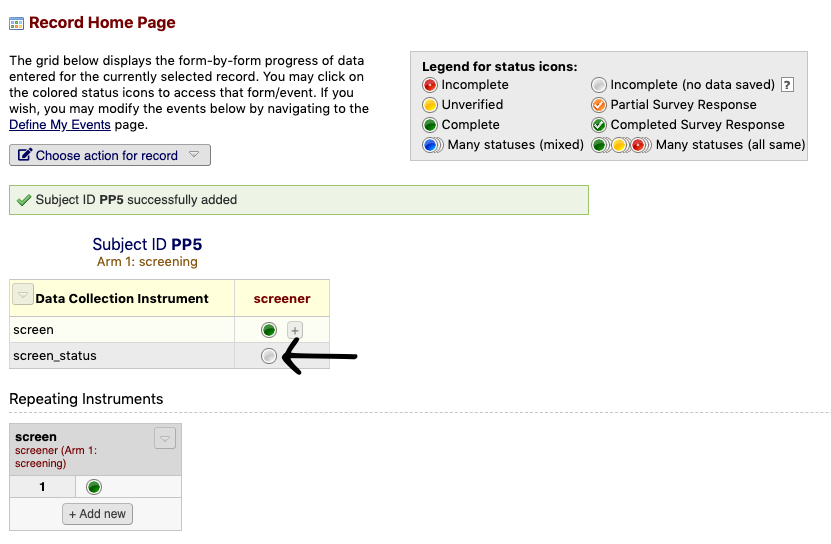
\includegraphics{images/redcap_screening/5.png}
  \end{itemize}
\item
  Click the screen\_status radio button
  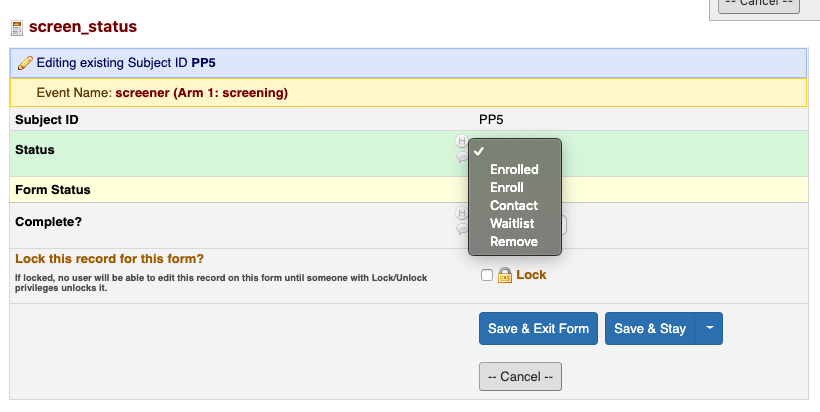
\includegraphics{images/redcap_screening/6.png}
\item
  Select the appropriate option

  \begin{itemize}
  \tightlist
  \item
    Contact - Participant needs to be re-contacted (add Recruitment Database \& ID Drive)
  \item
    Ineligible - Participant not eligible for study
  \item
    To Enroll - Participant to enroll (need to create subject ID, enter subject info, schedule participant, add to Recruitment Database, add to ID Drive)
  \item
    Enrolled - Participant has been enrolled (all above have been completed)
  \item
    To Remove - Participant wants to be removed
  \end{itemize}
\item
  Be sure to update the screen status after each contact

  \begin{itemize}
  \tightlist
  \item
    After 3 contacts (with no response) - review (time of day, contact method, etc.)
  \end{itemize}
\item
  If enrolled, proceed to pre-session checklist in the participant log
\end{enumerate}

\hypertarget{scheduling}{%
\subsubsection{Scheduling}\label{scheduling}}

\begin{enumerate}
\def\labelenumi{\arabic{enumi}.}
\tightlist
\item
  Open BabLab google calendar and note availability for designated data collection research team.
\item
  Check-in with the Lab Manager to see what the designated ``package mailing day'' of the week is.
  Participants must be scheduled 2 weeks or more in advance from the ``package mailing day'', to ensure appropriate time for the package to be received by the participant.
\item
  Create event on google calendar for 2 hours. Notify the participant that sessions may not last the full indicated time, however, we like to designate additional time just in case.
\item
  As soon as the participant has been scheduled, create/add to a google calendar event for the designated ``package mailing day'' of the week the participant ID (MBB number).
\item
  This will notify the Lab Manager to create a package for this participant with session and post-session materials when they go into the lab for ``package mailing day.''
\end{enumerate}

Making a Zoom link

\begin{enumerate}
\def\labelenumi{\arabic{enumi}.}
\tightlist
\item
  Log onto \url{https://zoom.us}
\item
  Click to ``Meetings'' and ``Schedule a new meeting'' \includegraphics{images/zoom_link/1.png}
\item
  Title the meeting with the Participant's MBB number, set scheduled time, indicate 3 hours \includegraphics{images/zoom_link/2.png}
\item
  Set setting with password and turn host/participant on \includegraphics{images/zoom_link/3.png}
\item
  Save and click to add Zoom meeting to google calendar \includegraphics{images/zoom_link/4.png}
\item
  Click on the \href{mailto:bablab.ucla@gmail.com}{\nolinkurl{bablab.ucla@gmail.com}} \includegraphics{images/zoom_link/5.png}
\item
  Click allow \includegraphics{images/zoom_link/6.png}
\item
  Copy the Zoom link from the Description section and save \includegraphics{images/zoom_link/7.png}
\item
  Paste Zoom link into the ``confirmation email'' you send to the participant with their session confirmation, Zoom instruction sheet, and Next Steps sheet
\end{enumerate}

\hypertarget{other-screening-information}{%
\subsubsection{Other Screening Information}\label{other-screening-information}}

Accessing Lists

To find out where participants are in the recruitment process, there are several lists.
\includegraphics{images/redcap_screening/7.png}
1. Click on ``Record Status Dashboard''
\includegraphics{images/redcap_screening/8.png}
2. Participants who have been enrolled will be listed in the Enrollment - Wave 1 list
3. Participants in the process of recruitment will be listed in one of the 4 Recruitment lists
- *These lists are populated based on the individuals ``Screen Status'' so be sure to update after each contact!

List Types

\begin{itemize}
\tightlist
\item
  Contact - List of individuals who need to be contacted or re-contacted (also includes waitlist)
\item
  Ineligible - Participants are ineligible but interested
\item
  To Enroll - Participants who have been screened and are eligible to enroll
\item
  To Remove - Participants who were not interested in being contacted for this or future research
\end{itemize}

\begin{center}\rule{0.5\linewidth}{0.5pt}\end{center}

\hypertarget{concerns}{%
\subsection{Concerns}\label{concerns}}

If a parent has a concern about the study before the session, send the email template:

\begin{itemize}
\tightlist
\item
  {[}MBB\_online - CONCERNS{]}
\end{itemize}

\begin{center}\rule{0.5\linewidth}{0.5pt}\end{center}

\hypertarget{online-session-preparation}{%
\subsection{Online Session Preparation}\label{online-session-preparation}}

\hypertarget{package-creation}{%
\subsubsection{Package creation}\label{package-creation}}

\begin{itemize}
\tightlist
\item
  There will be a designated ``package mailing day'' one day a week in which the Lab Manager will go into the lab to prepare necessary materials and send out packages from scheduled participants in the last week, on the same package mailing day.
\item
  Once the package has been created and sealed, it is time to bring the package down to Tyler's office in the Psychology building.
\item
  To mail the package to the participant, you will need the following information:

  \begin{itemize}
  \tightlist
  \item
    Recharge ID
  \item
    Participant name
  \item
    Participant mailing address
  \end{itemize}
\item
  From Tyler's office, you will receive a FedEx label in which you can write this information
\item
  Take a picture of the FedEx label and upload to Box
\item
  Leave the package in Tyler's office for FedEx pickup
\end{itemize}

\hypertarget{zoom-security-settings}{%
\subsubsection{Zoom security Settings}\label{zoom-security-settings}}

\begin{enumerate}
\def\labelenumi{\arabic{enumi}.}
\tightlist
\item
  Require Encryption for 3rd Party Endpoints*
\item
  Prevent participants from saving chat
\item
  Click on the ``security'' button and ensure the following items are checked and all other items unchecked \includegraphics{images/zoom_security/1.png}

  \begin{enumerate}
  \def\labelenumii{\alph{enumii}.}
  \tightlist
  \item
    ``Enable Waiting room''
  \item
    ``Lock Meeting'' after participant has entered
  \item
    Allow participant to ``Unmute Themselves''
  \end{enumerate}
\item
  Disable Cloud recording*
\item
  Host-only screen-sharing

  \begin{enumerate}
  \def\labelenumii{\alph{enumii}.}
  \tightlist
  \item
    click on the arrow next to ``screen sharing'' and click on ``Advanced sharing options'' \includegraphics{images/zoom_security/2.png}
  \item
    Ensure ``one participant can share at a time'' and ``only host'' options are selected \includegraphics{images/zoom_security/3.png}
  \end{enumerate}
\end{enumerate}

*Note that \#1 and \#4 are the default settings (so those don't have to be changed).

\begin{center}\rule{0.5\linewidth}{0.5pt}\end{center}

\hypertarget{online-session-protocols}{%
\section{Online Session Protocols}\label{online-session-protocols}}

\hypertarget{consent-assent-online}{%
\subsection{Consent \& Assent Online}\label{consent-assent-online}}

Once the parent and child/teen have connected with the researcher via Zoom, the researcher may begin the consenting (parent) and assenting (child aged 7+ or teen) process.

Make some small talk - Ask the participant how they got here. If they have participated before in research. Thank them for joining you via video call and for giving up their weekend to help science.

Tell the parent and child that the first thing you are going to do is go over all of the things they will do today, and have them fill out the consent and assent forms online.

Speak to them and direct them through the whole process.

Things you will do during the online session:

\begin{itemize}
\tightlist
\item
  Sit with parent and talk about fun things and hard things (filming).
\item
  Parent stays in room and answers more questions while child is working.
\item
  Child will play a computer game (look at pictures). Some of the pictures will be a little bit scary, others sad, others boring.
\item
  Parent will help child measure height, weight, and waist circumference.
\item
  Child will answer some questionnaires with researcher
\item
  Parent will help take two biological samples during the session:

  \begin{itemize}
  \tightlist
  \item
    Hair - stress hormones
  \item
    Saliva - microbiome
  \end{itemize}
\item
  You will get \$45 for the work you put in today
\end{itemize}

Things you will do at home (after the online session):

\begin{itemize}
\tightlist
\item
  Child Poop sample - microbiome
\item
  Stool scale
\item
  Memory game - to see what you remember from the session today
\item
  When you complete the poop sample and the game at home, we will pay you another \$20.
\end{itemize}

Things to know:

You are a volunteer, which means that you do not have to do anything, or say anything that makes you uncomfortable. We would like you to try everything you can, and to do your best, but if there are things you absolutely do not want to do, just tell us, that is o.k.

We keep your participation confidential - ID number.

We want you to come in again in the future, so we will ask for some information so we can contact you in the future.

Have the participant indicate consent/assent on REDCap consent form.

\begin{center}\rule{0.5\linewidth}{0.5pt}\end{center}

\hypertarget{parent-child-observation-online}{%
\subsection{Parent Child Observation Online}\label{parent-child-observation-online}}

The parent and child will be seated together in view on the Zoom camera. During that time they will be filmed while planning a conflict event, and then again while discussing a pleasant event. The conflict event will always go first, followed by the pleasant event. We did this to ensure that the parents were not thinking of the negative interaction upon answering the questionnaires about their child, which they did immediately after the observation interaction.

Step 1:
Researcher will ensure Zoom security settings are set up for the video.

\begin{itemize}
\tightlist
\item
  Parent and child will be situated side-by-side in view on the Zoom camera.
\item
  Researcher will rename the participant's name to the participant Secondary MBB ID number. \includegraphics{images/zoom_parent_child_interaction/1.png}
\item
  Researcher will ``hide self view'' \includegraphics{images/zoom_parent_child_interaction/2.png}
\end{itemize}

Step 2:
The researcher will ask the parent to find the \href{https://ucla.app.box.com/file/630327764749}{Pleasant/Unpleasant Events Checklist} piece of paper from their session package.

\emph{Researcher: Next we are going to take some film of you while you discuss a source of conflict (or something you disagree on) and try to resolve it. On this piece of paper is a list of things that parents and children sometimes have disagreements about. Please take a moment to read the list and think about some that you would like to discuss together. In about one minute, please start discussing the things you have selected from the list and try to resolve the areas of conflict you have chosen from the list. You do not need to tell us what you chose to discuss, and it does not matter if you chose something from the list, or decide to choose something else not included on the list. I am going to step out out of the room and away from the camera view, and silence my computer so I do not have a ``virtual presence'' during your conversation. I will give you five minutes to discuss the event, then I will come back into the video call and give you further instructions.}

Step 3:
Researcher press record on the Zoom application.\includegraphics{images/zoom_parent_child_interaction/3.png} Wait to hear the audio Zoom confirmation \emph{``this meeting is now being recorded''} and view recording in progress at top left of screen to ensure recording is live. \includegraphics{images/zoom_parent_child_interaction/4.png} Researcher turn down the volume on the computer and leave the room. Start timer for 6 minutes. At the end of 6 minutes, reenter camera view and turn up volume on researcher's computer.

\emph{Researcher: Thank you for taking the time to discuss the source of conflict and try to resolve it. Next we are going to take some film of you while you discuss a pleasant event you could do together. On your piece of paper is a list of events that parents and children sometimes find pleasant to do together. Please take a moment to read the list of events and think about what you would like to plan to do together. You do not need to tell us what you chose to discuss, and it does not matter if you chose something from the list, or decide to choose something else not included on the list. I am going to step out out of the room and away from the camera view once again, and silence my computer so I do not have a ``virtual presence'' during your conversation. I will give you five minutes to discuss the event, then I will come back into the video call and give you further instructions.}

Step 4:
Researcher keeps the recording going on Zoom and turns down the volume on the computer before leaving the room.

Step 5:
Researcher reenter the room and back into camera view, turn up volume on the computer, and stops the recording on Zoom. \includegraphics{images/zoom_parent_child_interaction/5.png} You will view this notification in the upper right hand corner that states the recorded file will be converted to mp4 once the meeting ends. \includegraphics{images/zoom_parent_child_interaction/6.png} Move the child/adolescent and parent onto the next task in the session, as the video will not be saved until after the session is complete.

\textbf{POST SESSION}

Step 6:
When the session is complete, click the bottom right hand button to end the meeting. \includegraphics{images/zoom_parent_child_interaction/7.png} You will immediately see this window pop up to indicate the recording is being converted and saving to your computer. \includegraphics{images/zoom_parent_child_interaction/8.png}
Step 7:
When the video conversion is complete, the video files will be saved in a folder titled ``Zoom'' on your computer, wherever your current automatic working directory is saved. \includegraphics{images/zoom_parent_child_interaction/9.png}
Step 8:
There will be three files in the folder- find the mp4 file and click open to ensure you have captured and converted the file successfully. \includegraphics{images/zoom_parent_child_interaction/10.png} Rename the file to the participant's secondary ID number, and upload to Box. \includegraphics{images/zoom_parent_child_interaction/11.png}

\begin{center}\rule{0.5\linewidth}{0.5pt}\end{center}

\hypertarget{parent-questionnaires-online}{%
\subsection{Parent Questionnaires Online}\label{parent-questionnaires-online}}

If the family has a second device available (smartphone, second computer, etc.) for the parent to begin questionnaires, advise the parent to REDCap and continue on these questionnaires during Child Halloween training and test, and Child questionnaires.

\hypertarget{parent-self-questionnaires}{%
\subsubsection{Parent Self Questionnaires}\label{parent-self-questionnaires}}

\begin{longtable}[]{@{}lll@{}}
\toprule
\begin{minipage}[b]{0.32\columnwidth}\raggedright
Title\strut
\end{minipage} & \begin{minipage}[b]{0.32\columnwidth}\raggedright
Description\strut
\end{minipage} & \begin{minipage}[b]{0.27\columnwidth}\raggedright
Reference\strut
\end{minipage}\tabularnewline
\midrule
\endhead
\begin{minipage}[t]{0.32\columnwidth}\raggedright
Beck Depression Inventory -- II (BDI-II) -- 13-18 years.\strut
\end{minipage} & \begin{minipage}[t]{0.32\columnwidth}\raggedright
Parent self-report. Domain assessed: mental health/affective functioning. Developed for the assessment of symptoms corresponding to criteria for diagnosing depressive disorders listed in the DSM IV.\strut
\end{minipage} & \begin{minipage}[t]{0.27\columnwidth}\raggedright
(ABC, XXXX)\strut
\end{minipage}\tabularnewline
\begin{minipage}[t]{0.32\columnwidth}\raggedright
COVID-19 Objective Questionnaire (covid\_objective)\strut
\end{minipage} & \begin{minipage}[t]{0.32\columnwidth}\raggedright
Parent self-report. Domains assessed: COVID-19 objective measures. This questionnaire consists of 12 items to identify health changes and lifestyle changes made From the impacts of the COVID-19 outbreak.\strut
\end{minipage} & \begin{minipage}[t]{0.27\columnwidth}\raggedright
(ABC, XXXX)\strut
\end{minipage}\tabularnewline
\begin{minipage}[t]{0.32\columnwidth}\raggedright
Parenting Stress\strut
\end{minipage} & \begin{minipage}[t]{0.32\columnwidth}\raggedright
Parent self-report. Domain assessed: parenting and family structure. The PSI designed to evaluate the magnitude of stress in the parent-child system, focusing on three major domains of stress: 1) child/adolescent characteristics, 2) parent characteristics, and 3) situational/demographic life stress. Revised questionnaire focuses on stress in the context of COVID-19.\strut
\end{minipage} & \begin{minipage}[t]{0.27\columnwidth}\raggedright
(ABC, XXXX)\strut
\end{minipage}\tabularnewline
\begin{minipage}[t]{0.32\columnwidth}\raggedright
COVID-19 Written Response- parent (optional)\strut
\end{minipage} & \begin{minipage}[t]{0.32\columnwidth}\raggedright
Domain assessed: Emotional impacts of COVID-19. This self-report measure consists of one long-form qualitative response, prompting a parent to write continuously for five minutes about the impacts of COVID-19 on their life and family. This qualitative response was adapted from previous prompts in writing about emotional experiences, and seeks to assess the emotional and behavioral impacts of the Pandemic on children and families.\strut
\end{minipage} & \begin{minipage}[t]{0.27\columnwidth}\raggedright
(ABC, XXXX)\strut
\end{minipage}\tabularnewline
\bottomrule
\end{longtable}

\hypertarget{parent-proxy-questionnaires}{%
\subsubsection{Parent Proxy Questionnaires}\label{parent-proxy-questionnaires}}

\begin{longtable}[]{@{}lll@{}}
\toprule
\begin{minipage}[b]{0.32\columnwidth}\raggedright
Title\strut
\end{minipage} & \begin{minipage}[b]{0.32\columnwidth}\raggedright
Description\strut
\end{minipage} & \begin{minipage}[b]{0.27\columnwidth}\raggedright
Reference\strut
\end{minipage}\tabularnewline
\midrule
\endhead
\begin{minipage}[t]{0.32\columnwidth}\raggedright
Demographic Questionnaire\strut
\end{minipage} & \begin{minipage}[t]{0.32\columnwidth}\raggedright
Parent proxy and self-report. Domain assessed: demographics. The project developed questionnaire asks parents about their household income, their own and their child's/adolescent's race/ethnicity, the parent age, education, and marital status, and contact details.\strut
\end{minipage} & \begin{minipage}[t]{0.27\columnwidth}\raggedright
(ABC, XXXX)\strut
\end{minipage}\tabularnewline
\bottomrule
\end{longtable}

\emph{coming soon\ldots{}}

\begin{center}\rule{0.5\linewidth}{0.5pt}\end{center}

\hypertarget{halloween-online}{%
\subsection{Halloween Online}\label{halloween-online}}

\emph{coming soon\ldots{}}

\begin{center}\rule{0.5\linewidth}{0.5pt}\end{center}

\hypertarget{height-online}{%
\subsection{Height Online}\label{height-online}}

\begin{itemize}
\tightlist
\item
  Researcher will be walking the parent through how to measure their child's height via Zoom video call. Ask parent if they have a full length measurement tape. If not, we will proceed with the paper measurement tape.
\item
  Ask parent to place child/adolescent directly against wall/frame
\item
  Advise child/adolescent to stand up straight
\item
  Have parent ensure heels of child/adolescent are up against the wall/frame
\item
  Use a flat object (booklet, ruler, sheet of paper, etc.) to accurately mark the height on the wall/frame
\item
  Use the paper measuring tape to scale up the wall and measure the height marking
\item
  Record height on Lab Session Checklist
\end{itemize}

\begin{center}\rule{0.5\linewidth}{0.5pt}\end{center}

\hypertarget{weight-online}{%
\subsection{Weight Online}\label{weight-online}}

\begin{itemize}
\tightlist
\item
  Instruct parent to have child/adolescent to step on weight scale
\item
  Measure weight
\item
  Record weight on Lab Session Checklist
\end{itemize}

\begin{center}\rule{0.5\linewidth}{0.5pt}\end{center}

\hypertarget{waist-measurement-online}{%
\subsection{Waist Measurement Online}\label{waist-measurement-online}}

\begin{itemize}
\tightlist
\item
  Advise parent to hold tape measure at the child/adolescent's belly button and bring it around their waist, over their t-shirt
\item
  Make sure measuring tape is horizontal around the waist and even in the front and back
\item
  Keep the tape snug around the waist, but not compressing the skin
\item
  Have participant breathe in
\item
  Measure the participant's waist just after they breathe out
\item
  Record waist measurement on Lab Session Checklist
\end{itemize}

\begin{center}\rule{0.5\linewidth}{0.5pt}\end{center}

\hypertarget{saliva-sample-collection-online}{%
\subsection{Saliva Sample Collection Online}\label{saliva-sample-collection-online}}

\begin{itemize}
\tightlist
\item
  Researcher has saliva ``spit tube'' example for explanation to participants
\item
  Advise parents to have child/adolescent fill spit tube to indicated line
\item
  Do not count the bubbles at the top, ensure that the saliva reaches the line
\item
  Close the cap on the saliva tube, to release the stabilizing solution and seal the sample
\item
  Put the sample in the biohazard bag with the two cotton balls inside
\item
  Put the biohazard bag with sample inside the rigid box and set aside for now
\end{itemize}

\begin{center}\rule{0.5\linewidth}{0.5pt}\end{center}

\hypertarget{hair-sample-collection-online}{%
\subsection{Hair Sample Collection Online}\label{hair-sample-collection-online}}

\hypertarget{set-up-hair-sample-station}{%
\subsubsection{Set Up Hair-Sample Station}\label{set-up-hair-sample-station}}

\begin{itemize}
\tightlist
\item
  Ask parent to gather the following materials for their ``hair-sample station'':

  \begin{itemize}
  \tightlist
  \item
    1 sheet of aluminum foil (provided)
  \item
    1 small ziplock bag with participant ID (provided)
  \item
    1 alcohol swab (provided)
  \item
    Painter-tape (provided)
  \item
    1 pair of gloves (provided)
  \item
    1 scissor (salon grade if they have)
  \item
    1 parting comb
  \item
    2 alligator curl clips (optional)
  \item
    1 hair claw clip (optional- for long hair)
  \item
    Hair sample picture directions
  \end{itemize}
\item
  Researcher set up the following materials (to help explain hair sample collection):

  \begin{itemize}
  \tightlist
  \item
    1 sheet of aluminum foil
  \item
    1 small ziplock bag with participant ID
  \item
    1 salon grade scissor
  \item
    1 wide and narrow tooth parting comb
  \item
    1 alcohol swab
  \item
    Painter-tape
  \item
    1 pair of gloves
  \item
    2 alligator curl clips
  \item
    1 hair claw clip (for long hair)
  \item
    Sample hair amount taken from wig
  \end{itemize}
\end{itemize}

\hypertarget{prior-to-getting-hair-sample-collection}{%
\subsubsection{Prior to Getting Hair Sample Collection}\label{prior-to-getting-hair-sample-collection}}

\begin{itemize}
\tightlist
\item
  Explain to both the child and parent that they will be collecting 30-50 strands of hair. The amount of hair to be collected is less hair than is lost in normal everyday-brushing from the back of the head.
\item
  Inform them how the site for the sampling is hidden by the surrounding hair, therefore not visible after collection.
\item
  Explain how the sample is used to measure a hormone called cortisol that is present in the hair.
\item
  Show on the hair sample picture directions sheet the hair sample taken from the wig to illustrate the amount of hair that will be collected (30-50 strands).
\item
  Offer to show our hair sample collection video
\end{itemize}

\hypertarget{hair-sample-prep}{%
\subsubsection{Hair Sample Prep}\label{hair-sample-prep}}

\begin{itemize}
\tightlist
\item
  Have parent use provided pair of gloves.
\item
  Wipe down the hair scissor/comb/clips with an alcohol swab.
\end{itemize}

\hypertarget{hair-length}{%
\subsubsection{Hair Length}\label{hair-length}}

\begin{itemize}
\tightlist
\item
  For short hair (less than 3cm), follow the Short-Hair Protocol below.
\item
  For medium-length hair (3-6cm), follow the Medium-Hair Protocol below.
\item
  For long hair (more than 6cm), follow the Long-Hair Protocol below.
\item
  Ideally, all hair sample should be at least 3cm long. If the hair is less than 1cm long, the sample cannot be used.
\end{itemize}

\textbf{Short-Hair Protocol (1-3cm)- advise parent to:}

\begin{itemize}
\tightlist
\item
  Take the comb and part the hair horizontally between the tips of the ears.
\item
  After parting, ask the participant to hold the parted hair close to the scalp.
\item
  Hold the loose hair tightly with index finger and thumb, and cut the hair along the part.
\item
  Place loose hairs in foil and fold it securely. Do NOT tape the hair to the foil.
\item
  Fold the foil without bending the hair, and ensure that the hair does not fall out of the foil.
\item
  Ensure the root-end on the aluminum foil is labeled and place it in the ziplock bag.
\item
  Ensure the ziplock bag is labeled with the participant's ID.
\end{itemize}

\textbf{Medium-Hair Protocol (3-6cm)- advise parent to:}

\begin{itemize}
\tightlist
\item
  Take the comb and part the hair horizontally between the tips of the ears.
\item
  Take a clip to clip away the hair from the top of the parting.
\item
  Place another clip at the bottom to expose a 5x10cm rectangle of loose hair between the two clips.
\item
  Ask if the child prefers the wide or narrow tooth comb to comb through the loose hair.
\item
  Ask if it is ok to discard any loose hair from the comb.
\item
  Grasp approx. 30-50 strands of hair to the right of the rectangle.
\item
  Gently pull and twist the hair away from the scalp in a rolling motion between the fingers.
\item
  Collect the sample as close to scalp as possible, but be careful to not cut the scalp.
\item
  Attach the hair to the center of the aluminum foil by taping with painter's tape - do not cover the root end.
\item
  Label the root end on the tape.
\item
  Fold the foil without bending the hair, and ensure that the hair does not fall out of the foil.
\item
  Ensure the root-end on the aluminum foil is labeled and place it in the ziplock bag.
\item
  Ensure the ziplock bag is labeled with the participant's ID.
\end{itemize}

\textbf{Long-Hair Protocol (\textgreater{} 6cm)- advise parent to:}

\begin{itemize}
\tightlist
\item
  Part the hair left to right at the posterior vertex.
\item
  Clip away any extra hair, then create a twist of hair and hold tightly with index finger and thumb.
\item
  Make a clean cut as close to scalp as possible.
\item
  If the hair is thin, cut 2-3 small areas (1cm apart) across the posterior vertex to conceal the site of the cut.
\item
  Attach the hair to the center of the aluminum foil by taping with painter's tape - do not cover the root end.
\item
  Label the root end on the tape.
\item
  Fold the foil without bending the hair, and ensure that the hair does not fall out of the foil.
\item
  Ensure the root-end on the aluminum foil is labeled and place it in the ziplock bag.
\item
  Ensure the ziplock bag is labeled with the participant's ID.
\end{itemize}

\begin{center}\rule{0.5\linewidth}{0.5pt}\end{center}

\hypertarget{child-questionnaires-online}{%
\subsection{Child Questionnaires Online}\label{child-questionnaires-online}}

\hypertarget{sharing-your-screen}{%
\subsubsection{Sharing Your Screen}\label{sharing-your-screen}}

\begin{itemize}
\tightlist
\item
  Researcher will open REDCap on their computer and enter in child code
\item
  On Zoom, click ``share screen'' with the participant \includegraphics{images/zoom_screenshare/1.png}
\item
  Be sure to indicate the correct screen to share, NOT sharing full desktop \includegraphics{images/zoom_screenshare/2.png}
\item
  Researcher will read through all questionnaires with children and indicate their responses on REDCap
\end{itemize}

\hypertarget{child-self-questionnaires}{%
\subsubsection{Child Self Questionnaires}\label{child-self-questionnaires}}

\begin{longtable}[]{@{}lll@{}}
\toprule
\begin{minipage}[b]{0.32\columnwidth}\raggedright
Title\strut
\end{minipage} & \begin{minipage}[b]{0.32\columnwidth}\raggedright
Description\strut
\end{minipage} & \begin{minipage}[b]{0.27\columnwidth}\raggedright
Reference\strut
\end{minipage}\tabularnewline
\midrule
\endhead
\begin{minipage}[t]{0.32\columnwidth}\raggedright
Alexithymia\strut
\end{minipage} & \begin{minipage}[t]{0.32\columnwidth}\raggedright
Child/adolescent self-report. Domain assessed: mental health/affective function. This questionnaire asks youth to endorse a number of items falling within three factors (1) Difficulty identifying feelings, (2) difficulty describing feelings, (3) externally oriented thinking.\strut
\end{minipage} & \begin{minipage}[t]{0.27\columnwidth}\raggedright
(Rieffe, Oosterveld, \& Terwogt, 2006)\strut
\end{minipage}\tabularnewline
\begin{minipage}[t]{0.32\columnwidth}\raggedright
Children's Perception of Interparental Conflict Scale (cpic)-- 6-18 years\strut
\end{minipage} & \begin{minipage}[t]{0.32\columnwidth}\raggedright
Child/adolescent self-report. Domains assessed: parenting and family structure. The CPIC assesses children's/adolescent's experience of parental conflict, including subscales (Conflict Properties, Threat, Self-Blame).\strut
\end{minipage} & \begin{minipage}[t]{0.27\columnwidth}\raggedright
(ABC, XXXX)\strut
\end{minipage}\tabularnewline
\begin{minipage}[t]{0.32\columnwidth}\raggedright
Child Somatization Symptom Inventory (cssi)-- 6-17 years\strut
\end{minipage} & \begin{minipage}[t]{0.32\columnwidth}\raggedright
Child/adolescent self-report. Parent report for children under 8 years. Domain assessed: physical symptoms. The CSSI assesses a variety of nonspecific somatic symptoms.\strut
\end{minipage} & \begin{minipage}[t]{0.27\columnwidth}\raggedright
(ABC, XXXX)\strut
\end{minipage}\tabularnewline
\begin{minipage}[t]{0.32\columnwidth}\raggedright
Security Scale (ss) -- 8-18 years\strut
\end{minipage} & \begin{minipage}[t]{0.32\columnwidth}\raggedright
Child/adolescent self-report. Domain assessed: attachment. This measure asks children/adolescents to endorse statements about their feelings towards their parents (in the positive or negative) and how much each endorsed statement is characteristic of them. Statements assess domains of being able to rely on parents in times of need, feelings of closeness with parent etc.\strut
\end{minipage} & \begin{minipage}[t]{0.27\columnwidth}\raggedright
(ABC, XXXX)\strut
\end{minipage}\tabularnewline
\begin{minipage}[t]{0.32\columnwidth}\raggedright
Benevolent Childhood Experiences Scale- Revised (bce)\strut
\end{minipage} & \begin{minipage}[t]{0.32\columnwidth}\raggedright
Child/adolescent self-report. Domain assessed: benevolent childhood experiences. This child/adolescent self-report questionnaire consists of 10 items used to identify favorable childhood experiences, with regards to potential child adversity.\strut
\end{minipage} & \begin{minipage}[t]{0.27\columnwidth}\raggedright
(ABC, XXXX)\strut
\end{minipage}\tabularnewline
\begin{minipage}[t]{0.32\columnwidth}\raggedright
COVID-19 Written Response- child (optional)\strut
\end{minipage} & \begin{minipage}[t]{0.32\columnwidth}\raggedright
Domain assessed: Emotional impacts of COVID-19. This self-report measure consists of one long-form qualitative response, prompting a child to write continuously for five minutes about the impacts of COVID-19 on their life and family (for children who cannot write or do not feel comfortable writing, children can dictate and parent can write). This qualitative response was adapted from previous prompts in writing about emotional experiences, and seeks to assess the emotional and behavioral impacts of the Pandemic on children and families.\strut
\end{minipage} & \begin{minipage}[t]{0.27\columnwidth}\raggedright
(ABC, XXXX)\strut
\end{minipage}\tabularnewline
\bottomrule
\end{longtable}

\begin{center}\rule{0.5\linewidth}{0.5pt}\end{center}

\hypertarget{home-sessionlast-checks}{%
\subsection{Home Session/Last Checks}\label{home-sessionlast-checks}}

\begin{itemize}
\tightlist
\item
  BSS sheet
\item
  Stool Sample explanation

  \begin{itemize}
  \tightlist
  \item
    There is a toilet hat and a gut kit in the session package
  \end{itemize}
\item
  Contact list explanation

  \begin{itemize}
  \tightlist
  \item
    \emph{In a longitudinal study, information may change in time and we want to ensure we have a way to recontact you for the next wave if you are still interested in joining}
  \end{itemize}
\item
  Schedule time to complete post-session tasks \textasciitilde{}1 week post-session

  \begin{itemize}
  \tightlist
  \item
    Create MBB calendar event to send home session reminder 1 (email) (on the day that home session is scheduled)
  \item
    Create MBB calendar event to make home session reminder 1 (call) (2 days after scheduled home session)
  \item
    Create MBB calendar event to send home session reminder 2 (email) (4 days after scheduled home session)
  \item
    Create MBB calendar event to send home session reminder 3 (email) (6 days after scheduled home session)
  \end{itemize}
\item
  Payment

  \begin{itemize}
  \tightlist
  \item
    Confirm mailing address
  \item
    Explain that once the return mailer has been received to the lab, we will send payment through the mail along with a few educational science kits
  \end{itemize}
\end{itemize}

\begin{center}\rule{0.5\linewidth}{0.5pt}\end{center}

\hypertarget{qualitative-responses}{%
\subsection{Qualitative Responses}\label{qualitative-responses}}

\begin{itemize}
\tightlist
\item
  Two qualitative free responses on REDCap are optional, and should be offered to parents and children to complete if they are interested
\item
  These qualitative responses require five minutes of continued writing to capture the impacts of COVID-19 on families, caregivers, and children
\item
  If interested, researcher will send the REDCap link and codes for parent and child to complete
\end{itemize}

\begin{center}\rule{0.5\linewidth}{0.5pt}\end{center}

\hypertarget{post-online-session-protocols}{%
\section{Post-Online Session Protocols}\label{post-online-session-protocols}}

\hypertarget{parent-child-observation-online-coding}{%
\subsection{Parent Child Observation Online Coding}\label{parent-child-observation-online-coding}}

\hypertarget{coding-the-interview}{%
\subsubsection{Coding the interview}\label{coding-the-interview}}

\begin{itemize}
\item
  After the interviews are collected, videos will be coded by two observers blind to the caregiving group of the child (adversity or comparison).
\item
  Our original plan was to follow the LIFE coding system developed by Hops:

  \begin{itemize}
  \tightlist
  \item
    Hops H, Davis B, Longoria N. Methodological issues in direct observation -- Illustrations with the Living in Familial Environments (LIFE) coding system. Journal of Clinical Child Psychology. 1995;24:193--203. \href{https://www.tandfonline.com/doi/abs/10.1207/s15374424jccp2402_7?journalCode=hcap19}{Google Scholar}
  \end{itemize}
\item
  However, this system is prohibitively expensive and very training intensive. Instead we decided to go with either of the following two coding schedules:

  \begin{itemize}
  \item
    \begin{enumerate}
    \def\labelenumi{\arabic{enumi}.}
    \tightlist
    \item
      Family Interaction Macrocoding Schedule (FIMS) Holmbeck, Zebracki, Johnson, Belvedere, \& Hommeyer, 2007.
    \end{enumerate}
  \item
    \begin{enumerate}
    \def\labelenumi{\arabic{enumi}.}
    \setcounter{enumi}{1}
    \tightlist
    \item
      CIB Training with Ruth Feldman.
    \end{enumerate}
  \end{itemize}
\item
  We ultimately decided to go with FIMS for several reasons:

  \begin{itemize}
  \tightlist
  \item
    Expense - Sarah Whittle paid approximately \$ 1000USD for a 10 hour skype training session with one of Holmbeck's team), whereas CIB training is /\$2500 and also involves flights and accommodation at Yale.
  \item
    Validation in age range - I like CIB for younger children, but FIMS was designed for older children and adolescents, and Sarah Whittle has validated it in a community sample of 8 year olds and their mothers.
  \item
    FIMS is a less intensive coding schedule, producing global codes, rather than micro coded (i.e., minute to minute) scales - which makes more intuitive sense in the age range for MBB.
  \item
    FIMS has a peer version that we might brach out to in the future (but likely not needing further training): \url{https://psycnet.apa.org/record/2014-24011-001}
  \item
    Sarah Whittle's group looked at the component structure for the FIMS and found components that seemed close to what they were finding with the Hops LIFE system - namely: negative maternal affect during pleasant event, negative maternal during conflict discussion, and pleasant maternal affect across both tasks (warmth). The negative maternal during pleasant event was the most predictive of child behavior problems. Overall, the correlations they report in their paper are all very sensical and convinced me that we should use the FIMS. \url{https://journals.sagepub.com/doi/full/10.1177/1073191118796557}
  \end{itemize}
\end{itemize}

\begin{center}\rule{0.5\linewidth}{0.5pt}\end{center}

\hypertarget{saliva-sample-storage}{%
\subsection{Saliva Sample Storage}\label{saliva-sample-storage}}

\begin{itemize}
\tightlist
\item
  Screw lids on very tight (to prevent evaporation)
\item
  Log the location (grid) on the sample storage log
\end{itemize}

\begin{center}\rule{0.5\linewidth}{0.5pt}\end{center}

\hypertarget{hair-sample-storage}{%
\subsection{Hair Sample Storage}\label{hair-sample-storage}}

\begin{itemize}
\tightlist
\item
  Store the sample in a dry area at room temperature
\end{itemize}

\begin{center}\rule{0.5\linewidth}{0.5pt}\end{center}

\hypertarget{stool-sample-storage}{%
\subsection{Stool Sample Storage}\label{stool-sample-storage}}

\hypertarget{sample-quality}{%
\subsubsection{Sample Quality}\label{sample-quality}}

\begin{itemize}
\tightlist
\item
  Put on gloves.
\item
  Open the mailer to ensure that it contains both the stool sample (in biohazard bag) and the Bristol Stool Scale.
\item
  Check for quality of the stool sample by shaking it up and down vigorously (keep the sample in the biohazard bag), then check for its consistency and color - It should be a dark-brown liquid.
\item
  If stool sample does not meet requirement (e.g.~sample is in solid form or amount collected is too little), contact the family to see if they would be willing to send another sample with compensation.
\item
  Contact family if the Bristol Stool Scale is missing in the mailer.
\end{itemize}

\hypertarget{sample-transfer}{%
\subsubsection{Sample Transfer}\label{sample-transfer}}

\begin{itemize}
\tightlist
\item
  Wear appropriate PPE:

  \begin{itemize}
  \tightlist
  \item
    Gloves
  \item
    Lab coat
  \item
    Safety glasses
  \item
    Surgical Mask
  \item
    Closed-toe shoes
  \item
    Long pants
  \item
    Hair tied back
  \end{itemize}
\item
  Prepare your station and ensure that you have the following:

  \begin{itemize}
  \tightlist
  \item
    Drape
  \item
    2.0mL cryogenic vials
  \item
    Stool samples in biohazard bag
  \item
    Test tube racks
  \item
    Transport box with divider
  \item
    Sharpie for labeling
  \end{itemize}
\end{itemize}

\textbf{Steps:}

\begin{itemize}
\tightlist
\item
  Lay a new drape on the work station and keep all equipments and sample on the drape throughout the transfer process.
\item
  With the stool sample collection vial still in the biohazard bag, shake it up and down vigorously.
\item
  Take the stool sample out of the bag and put it on the test tube rack.
\item
  Untwist two 2.0mL vials and place them on the test tube rack.
\item
  Untwist the stool sample collection vial, and carefully pour the sample into the first 2.0mL vial. (It's okay if the ball does or does not get transferred)
\item
  Stop pouring when solution reached the 1.8mL line to prevent overflow, and pour the remaining sample (if any) in a second 2.0mL vial.
\item
  Cap the 2.0mL vials tightly to prevent spills.
\item
  Label the 2.0mL vials with a sharpie, ensure it has the participant ID and vial number.
\item
  Place the labeled 2.0mL vials in the transport box with divider.
\item
  Close the now-empty stool sample collection vial, put it back in the biohazard bag, and dispose it in the biohazard waste bin.
\item
  Clean up work station, dispose the drape, and wipe down the table top with disinfectant wipe.
\item
  Remove PPE and wash hands with soap and water thoroughly.
\item
  Bring the transport box to C454 where the -80˚C freezer is located (key in BABLab Lock Box).
\item
  Place the 2.0mL vials in their designated space in the freezer box (in accordance to the Sample Storage Log Diagram).
\item
  Log the sample in the \href{https://app.box.com/file/630322897864}{Sample Storage Log}.
\end{itemize}

\begin{center}\rule{0.5\linewidth}{0.5pt}\end{center}

\hypertarget{data-entry-quality}{%
\subsection{Data Entry \& Quality}\label{data-entry-quality}}

\hypertarget{data-entry}{%
\subsubsection{Data Entry}\label{data-entry}}

\hypertarget{data-quality}{%
\subsubsection{Data Quality}\label{data-quality}}

\begin{center}\rule{0.5\linewidth}{0.5pt}\end{center}

\hypertarget{data-review-audit-online}{%
\subsection{Data Review \& Audit Online}\label{data-review-audit-online}}

\hypertarget{follow-up-completed-by-scheduling-coordinator}{%
\subsubsection{Follow-Up (completed by Scheduling Coordinator)}\label{follow-up-completed-by-scheduling-coordinator}}

\begin{itemize}
\tightlist
\item
  Before sending Home Reminder 3, make sure RA's have completed Data Entry, Data Quality Check 1, and Data Quality Check 2.
\item
  After sending Home Reminder 3 - create blank Trello card for participant on ``In Data Review'' list of Data Audit Board.
\end{itemize}

\hypertarget{data-review}{%
\subsubsection{Data Review}\label{data-review}}

\begin{itemize}
\tightlist
\item
  Once card has been created, do Data Review.
\item
  Checking for completion of:

  \begin{itemize}
  \tightlist
  \item
    child questionnaires (see child questionnaire table)
  \item
    parent proxy questionnaires (see parentproxy questionnaire table)
  \item
    parent self questionnaires (see parentself questionnaire table)
  \item
    hair sample
  \item
    saliva sample
  \item
    stool sample
  \item
    bss sheet
  \item
    contact sheet
  \item
    halloween delay test
  \item
    height, weight, waist
  \item
    PC interaction video
  \item
    halloween training and test data captured
  \end{itemize}
\item
  After completing Data Review, move card to Good Sample, Bad Sample, or No Sample list based on the stool sample.
\end{itemize}

\hypertarget{data-audit}{%
\subsubsection{Data Audit}\label{data-audit}}

\textbf{If Good Sample:}

\begin{itemize}
\tightlist
\item
  Send payment, thank you letter, certificate, and science kits via mail
\item
  Send {[}MBB - PAID{]} email and attach thank you letter, certificate, and parent report (including outstanding items).
\item
  Move to Paid list.
\item
  One week after payment is sent, check outstanding items and do Audit Call \#1.
\item
  One week following Audit Call \#1, check outstanding items do Audit Call \#2.
\item
  Within 2 days, check outstanding items and do Audit Call \#3.
\item
  After Audit Call \#3 (or all items completed), send {[}MBB - DONE{]} email and move to Done list.
\end{itemize}

\textbf{If Bad Sample:}

\begin{itemize}
\tightlist
\item
  Send payment, thank you letter, certificate, and science kits via mail. Include a new stool sample kit.
\item
  Send {[}MBB - PAID{]} email and attach thank you letter, certificate, and parent report (including outstanding items - emphasize stool sample kit).
\item
  Move to Paid list in Trello.
\item
  One week after payment is sent, check outstanding items do Audit Call \#1.
\item
  One week following Audit Call \#1, check outstanding items do Audit Call \#2.
\item
  Within 2 days, check outstanding items and do Audit Call \#3.
\item
  After Audit Call \#3 (or all items completed), send {[}MBB - DONE{]} email and move to Done list.
\end{itemize}

\textbf{If No Sample:}

\begin{itemize}
\tightlist
\item
  Send {[}MBB - UNPAID{]} email and attach thank you letter, certificate, and parent report (including outstanding items - emphasize stool sample kit).
\item
  Leave participant on Unpaid list.
\item
  If stool sample recieved - send payment, thank you letter, certificate, and science kits via mail and move to Paid list.
\item
  If stool sample not received, one week after email is sent, check outstanding items do Audit Call \#1.
\item
  One week following Audit Call \#1, check outstanding items do Audit Call \#2.
\item
  Within 2 days of Audit Call \#2, check outstanding items and do Audit Call \#3.
\item
  After Audit Call \#3 (or all items completed), send {[}MBB - DONE{]} email and move to Done list.
\end{itemize}

\hypertarget{getting-a-code-from-redcap}{%
\subsubsection{Getting A Code From REDCap}\label{getting-a-code-from-redcap}}

\begin{enumerate}
\def\labelenumi{\arabic{enumi}.}
\tightlist
\item
  Log onto REDCap and click on ``record status dashboard''
\end{enumerate}

\includegraphics{images/redcap_code/1.png}
2. Click on designated participant

\includegraphics{images/redcap_code/2.png}
3. Click on the first incomplete questionnaire for the parentself, parentproxy, or child questionnaire sets

\includegraphics{images/redcap_code/3.png}
4. Click on Survey Options

\includegraphics{images/redcap_code/4.png}
5. Click Survey Access Code and QR Code

\includegraphics{images/redcap_code/5.png}
6. Copy and paste web address and code + send to email to participant

\hypertarget{report-card-instructions}{%
\subsubsection{Report Card Instructions}\label{report-card-instructions}}

\begin{enumerate}
\def\labelenumi{\arabic{enumi}.}
\tightlist
\item
  Open a participant data folder
\end{enumerate}

\begin{figure}
\centering
\includegraphics{images/report_card_online/1.png}
\caption{}
\end{figure}

\begin{enumerate}
\def\labelenumi{\arabic{enumi}.}
\setcounter{enumi}{1}
\tightlist
\item
  Navigate to the report card folder and rename the template file - MBB999 to the relevant participant - and open the file
\end{enumerate}

\begin{figure}
\centering
\includegraphics{images/report_card_online/2.png}
\caption{}
\end{figure}

\begin{enumerate}
\def\labelenumi{\arabic{enumi}.}
\setcounter{enumi}{2}
\tightlist
\item
  Navigate to the last pge of the pdf and fill in the scores for this participant. You can type directly on the page- it is a fillable form.
\end{enumerate}

\begin{figure}
\centering
\includegraphics{images/report_card_online/3.png}
\caption{}
\end{figure}

\begin{enumerate}
\def\labelenumi{\arabic{enumi}.}
\setcounter{enumi}{3}
\tightlist
\item
  After you have entered teh data, it should look like this:
\end{enumerate}

\textbf{photo coming soon}

\begin{enumerate}
\def\labelenumi{\arabic{enumi}.}
\setcounter{enumi}{4}
\tightlist
\item
  If there are any comments, enter them on the comments page.
\end{enumerate}

\begin{itemize}
\tightlist
\item
  For example, if any NA's are present due to less than 70\% of data for that subset being available to calculate a score - note that here.
\item
  If there are no comments, delete this page.
  \includegraphics{images/report_card_online/5.png}
\end{itemize}

\begin{enumerate}
\def\labelenumi{\arabic{enumi}.}
\setcounter{enumi}{5}
\tightlist
\item
  \textbf{Important}- Once you have completed the edits to the pdf, you must follow these steps to ``lock'' the data so that it is no longer editable before sending to the participant. To do so, click file/print/PDF/Save as PDF. Save the PDF to your desktop, then replace the original PDF with the desktop version.
\end{enumerate}

\begin{figure}
\centering
\includegraphics{images/report_card_online/6.png}
\caption{}
\end{figure}

\begin{enumerate}
\def\labelenumi{\arabic{enumi}.}
\setcounter{enumi}{6}
\tightlist
\item
  The report card is now ready to be sent to the participant.
\end{enumerate}

\begin{center}\rule{0.5\linewidth}{0.5pt}\end{center}

\hypertarget{payment}{%
\subsection{Payment}\label{payment}}

\textbf{Payment package contents:}

\begin{itemize}
\tightlist
\item
  Payment box
\item
  Type in participant's name and print copy of certificate
\item
  Print thank you letter
\item
  Include \$65 Amazon gift card
\item
  Check stool sample quality- if poor, send another stool kit
\item
  Science kit- Neuron

  \begin{itemize}
  \tightlist
  \item
    4 pipe cleaners
  \item
    Pipe Cleaner Neuron photo directions quarter sheets
  \item
    goodie bag + tie
  \end{itemize}
\item
  Science kit- Brain hat

  \begin{itemize}
  \tightlist
  \item
    left + right side brain hat sheet
  \item
    Brain hat photo directions quarter sheets
  \item
    plastic sheet cover
  \end{itemize}
\item
  Science kit- Petri Dish

  \begin{itemize}
  \tightlist
  \item
    petri dish sheet
  \item
    Microbiome photo directions quarter sheets
  \item
    plastic sheet cover
  \item
    virus stickers
  \end{itemize}
\end{itemize}

\textbf{Mailing payment package}

\begin{itemize}
\tightlist
\item
  Once the package has been created and sealed, it is time to bring the package down to Tyler's office in the Psychology building.
\item
  To mail the package to the participant, you will need the following information:

  \begin{itemize}
  \tightlist
  \item
    Recharge ID
  \item
    Participant name
  \item
    Participant mailing address
  \end{itemize}
\item
  From Tyler's office, you will receive a FedEx label in which you can write this information
\item
  Take a picture of the FedEx label and upload to Box
\item
  Leave the package in Tyler's office for FedEx pickup
\end{itemize}

\textbf{Recording Payment}

\begin{itemize}
\tightlist
\item
  Log participant payment in reimbursement log book
\item
  Log participant payment in reimbursement spreadsheet
\end{itemize}

\begin{center}\rule{0.5\linewidth}{0.5pt}\end{center}

\hypertarget{sona-collection}{%
\chapter{SONA Collection}\label{sona-collection}}

\hypertarget{sona-collection-summary}{%
\section{SONA Collection Summary}\label{sona-collection-summary}}

Additional data collection of the 2 part Halloween task (for immediate and delayed testing of the memory task) will be taken with participants aged 18+. We project collecting from 250 participants (due to potential attrition of the 2 part task) and will compensate participants with school credit on the SONA system.

\begin{center}\rule{0.5\linewidth}{0.5pt}\end{center}

\hypertarget{sona-collection-measures}{%
\section{SONA Collection Measures}\label{sona-collection-measures}}

\hypertarget{sona-questionnaires}{%
\subsection{SONA Questionnaires}\label{sona-questionnaires}}

\begin{longtable}[]{@{}lll@{}}
\toprule
\begin{minipage}[b]{0.32\columnwidth}\raggedright
Title\strut
\end{minipage} & \begin{minipage}[b]{0.32\columnwidth}\raggedright
Description\strut
\end{minipage} & \begin{minipage}[b]{0.27\columnwidth}\raggedright
Reference\strut
\end{minipage}\tabularnewline
\midrule
\endhead
\begin{minipage}[t]{0.32\columnwidth}\raggedright
Demographic Questionnaire\strut
\end{minipage} & \begin{minipage}[t]{0.32\columnwidth}\raggedright
Adult self-report. Domain assessed: demographics. The project developed questionnaire asks participants about their household income, their race/ethnicity, the parent age, education, and marital status, and contact details.\strut
\end{minipage} & \begin{minipage}[t]{0.27\columnwidth}\raggedright
(ABC, XXXX)\strut
\end{minipage}\tabularnewline
\begin{minipage}[t]{0.32\columnwidth}\raggedright
Revised Childhood Traumatic Experiences Survey (cte\_revised) -- 18+ years of age.\strut
\end{minipage} & \begin{minipage}[t]{0.32\columnwidth}\raggedright
Adult report. Domain assessed: Traumatic Experiences. The Childhood Trauma Questionnaire is a brief 6 item survey of retrospectively-reported traumatic experiences (death, divorce, violence, sexual abuse, illness, and upheaval).\strut
\end{minipage} & \begin{minipage}[t]{0.27\columnwidth}\raggedright
(ABC, XXXX)\strut
\end{minipage}\tabularnewline
\bottomrule
\end{longtable}

\begin{center}\rule{0.5\linewidth}{0.5pt}\end{center}

\hypertarget{references}{%
\chapter{References}\label{references}}

Callaghan, B. L., Fields, A., Gee, D. G., Gabard-Durnam, L., Caldera, C., Humphreys, K. L., Goff, B., Flannery, J., Telzer, E. H., Shapiro, M., \& Tottenham, N. (2020). Mind and gut: Associations between mood and gastrointestinal distress in children exposed to adversity. \emph{Development and Psychopathology}, \emph{32}(1), 309--328. \url{https://doi.org/10.1017/S0954579419000087}

Callaghan, Dandesh, \ldots{} Whittle. Amygdala Resting Connectivity Mediates Association Between Maternal Aggression and Adolescent Major Depression: A 7-Year Longitudinal Study. \emph{JACPP} \href{https://www.jaacap.org/article/S0890-8567(17)31673-8/fulltext}{Google Scholar}

Hops H., Davis B., Longoria N. (1995) Methodological issues in direct observation -- Illustrations with the Living in Familial Environments (LIFE) coding system. \emph{Journal of Clinical Child Psychology}, 24:193--203.

MacPhillamy D. J., \& Lewinsohn P. M. Manual for the Pleasant Events Schedule. Eugene, OR: University of Oregon; 1976. \href{https://scholar.google.com/scholar_lookup?title=Manual+for+the+Pleasant+Events+Schedule\&author=DJ+MacPhillamy\&author=PM+Lewinsohn\&publication_year=1976\&}{Google Scholar}

Robin A. L. (1975). Communication Training: A Problem Solving Approach to Parent-Adolescent Conflict. Unpublished doctoral dissertation. State University of New York, Stony Brook.

Robin A. L., \& Foster S. L. (1989). \emph{Negotiating Parent-Adolescent Conflict: A Behavioral-Family Systems Approach}. New York, NY: Guilford Press.

Whittle, S., Yap, M. B. H., {[}\ldots{}{]}, \& Allen, N. B. (2009) Maternal responses to adolescent positive affect are associated with adolescents' reward neuroanatomy. \emph{Social Cognitive and Affective Neuroscience}. \href{https://www.ncbi.nlm.nih.gov/pmc/articles/PMC2728631/}{Google Scholar}

Whittle, S., Simmons, J. G., {[}\ldots{}{]}, \& Allen, N. B. (2014). Positive parenting predicts the development of adolescent brain structure: A longitudinal study. \emph{Developmental Cognitive Neuroscience}. \href{https://www.sciencedirect.com/science/article/pii/S1878929313000650}{Google Scholar}

Xie, Yihui. 2015. Dynamic Documents with R and Knitr. 2nd ed. Boca Raton, Florida: Chapman; Hall/CRC. \url{http://yihui.name/knitr/}.

\url{https://www.brightfutures.org/mentalhealth/pdf/professionals/ad/issues.pdf}

\hypertarget{questionnaire-references}{%
\section{Questionnaire References}\label{questionnaire-references}}

Rieffe, C., Oosterveld, P., \& Terwogt, M. M. (2006). An alexithymia questionnaire for children: Factorial and concurrent validation results. Personality and individual differences, 40(1), 123-133. \href{https://www.sciencedirect.com/science/article/abs/pii/S019188690500231X}{Google Scholar}

\bibliography{book.bib,packages.bib}

\end{document}
